\documentclass[a4paper,11pt]{article}
\usepackage{jheppub}
\usepackage{graphicx}% Include figure files
\usepackage{graphics}
\usepackage{dcolumn}% Align table columns on decimal point
\usepackage{bm}% bold math
\usepackage{epstopdf}
\usepackage{mathrsfs}
\usepackage{amssymb}
\usepackage{amsmath}
%\usepackage[pdftex]{hyperref}
\usepackage{natbib}

\def\bs{\boldsymbol}
\def\del{\partial}

%\def\p{{\boldsymbol p}_{\perp }}
%\def\pb{\bar {\boldsymbol p}_{\perp }}
%\def\pp{{\boldsymbol p}_{\perp }}
\def\p{{\boldsymbol p}}
\def\pb{\bar {\boldsymbol p}}
\def\pp{{\boldsymbol p}}
%\def\q{{\boldsymbol q}_\perp}
\def\q{{\boldsymbol q}}
\def\l{{\boldsymbol l}_\perp}
%\def\k{{\boldsymbol k}_\perp}
\def\k{{\boldsymbol k}}
\def\m{{\boldsymbol m}_\perp}
%\def\x{{\boldsymbol x}_\perp}
\def\x{{\boldsymbol x}}
\def\y{{\boldsymbol y}_\perp}
\def\X{{\boldsymbol X}_\perp}
\def\Y{{\boldsymbol Y}_\perp}
\def\D{{\boldsymbol D}_\perp}
\def\r{{\boldsymbol r}_\perp}
\def\z{{\boldsymbol z}_\perp}
%\def\v{{\boldsymbol v}_\perp}
\def\v{{\boldsymbol v}}
\def\w{{\boldsymbol w}_\perp}
\def\b{{\boldsymbol b}_\perp}
\def\Q{{\boldsymbol Q}_\perp}
\def\M{{\boldsymbol M}_\perp}
%\def\bkappa{{\boldsymbol \kappa}_\perp}
%\def\bbkappa{\bar{\boldsymbol \kappa}_\perp}
\def\bkappa{{\boldsymbol \kappa}}
\def\bbkappa{\bar{\boldsymbol \kappa}}
\def\bnu{{\boldsymbol \nu}_\perp}
\def\V{\hat{\boldsymbol v}_{1\perp}}
\def\K{\hat{\boldsymbol k}_{1\perp}}
\def\bV{\hat{\boldsymbol v}_{2\perp}}
\def\bK{\hat{\boldsymbol k}_{2\perp}}
\def\qqb{{q\bar q}}
\def\sM{{\scriptscriptstyle M}}

\newcommand{\beq}{\begin{eqnarray}}
\newcommand{\eeq}{\end{eqnarray}}
\newcommand{\be}{\begin{equation}}
\newcommand{\ee}{\end{equation}}
\newcommand{\nn}{\nonumber\\ }
\newcommand{\labe}{\label}
\newcommand{\bea}{\begin{eqnarray}}
\newcommand{\eea}{\end{eqnarray}}


\newcommand{\la}{\left\langle}
\newcommand{\ra}{\right\rangle}
\newcommand{\lc}{\left[}
\newcommand{\rc}{\right]}
\newcommand{\lp}{\left(}
\newcommand{\rp}{\right)}

\bibliographystyle{JHEP}
\usepackage{multirow}

\title{Boosting Higgs Pair Production in the $bb\bar{b}\bar{b}$ Channel at the LHC with Multivariate Techniques}

\author[a]{Katharina Behr, Nurfiki Bin Norjoharuddeen, Daniela Bortoletto, James Frost, Nathan P. Hartland, Cigdem Issever and Juan Rojo}

\affiliation[a]{Physics Department, 1 Keble Road, University of Oxford, United Kingdom }

\emailAdd{cigdem.issever@physics.ox.ac.uk}

\preprint{OUTP-15-14P}

\abstract{
  The measurement of Higgs pair production is one of the cornerstones of
  the LHC program for the next years.
  %
  Double Higgs production provides a unique window to the electroweak
  symmetry breaking mechanism, in particular to the Higgs trilinear coupling.
  %
  In this work we study the feasibility of the observation of the production of
  Higgs boson pairs at the High-Luminosity LHC using the
  $bb\bar{b}\bar{b}$ final state.
  %
  While the signal in this channel
  is enhanced by the large branching fraction of Higgs bosons to
  $b\bar{b}$ pairs, this measurement is  challenging due to the
  overwhelming QCD multijet background.
  %
  Our analysis is based on the combination of traditional cut-based
  methods and modern multivariate techniques, which lead to a substantial
  enhacement of the signal significance.
  %
  By combining the contribution from the boosted, intermediate and resolved
  topologies we achieve $S/\sqrt{B}=3.8$.
  %
  Therefore, we demonstrate that at the HL-LHC the $b\bar{b}b\bar{b}$ channel alone
  should allow to claim evidence of the observation of double Higgs production.
}


\begin{document} 
\maketitle

\flushbottom

\section{Introduction}

The measurement of double Higgs production will be one of the central
physics goals of the LHC program in its recently started high-energy
phase, as well as for its future high-luminosity upgrade (HL-LHC)
which aims to accumulate a total integrated
luminosity of 3 ab$^{-1}$~\cite{ATLAS:2013hta,CMS:2013xfa}.
%
Higgs pair production is directly sensitive to the
Higgs trilinear coupling $\lambda$~\cite{baglio} and 
provides crucial
information on the electroweak symmetry breaking mechanism.
%
It also probes the underlying strength of the Higgs interactions
at high energies, and can be used to test the composite nature of the 
Higgs boson~\cite{Giudice:2007fh,Contino:2010mh}.
%
While Standard Model (SM) cross-sections are small,
many Beyond the SM (BSM)
scenarios predict enhanced rates for double Higgs production, therefore searches have already been performed by ATLAS and CMS with Run I data~\cite{Aad:2015xja,Aad:2015uka,Aad:2014yja,Khachatryan:2015yea,Chatrchyan:2011wt}
and will continue at Run II.
%
The study of Higgs pair production will also be relevant to
any future high-energy 
collider, either at a 100 TeV circular machine~\cite{Arkani-Hamed:2015vfh,Barr:2014sga,Papaefstathiou:2015iba,Azatov:2015oxa} or at
a linear or circular electron-positron collider~\cite{Contino:2013gna}.

Analogously to single Higgs production~\cite{Dittmaier:2012vm}, 
in the SM the dominant mechanism for the production of a pair of
Higgs bosons at the LHC is 
gluon fusion (see Refs.~\cite{baglio,Frederix:2014hta} and
references therein).
%
For a center-of-mass energy of $\sqrt{s} = 14\,$TeV, the
next-to-next-to-leading order (NNLO)
total cross section is approximately $40\,$fb~\cite{deFlorian:2013jea},
which is increased by a further few percent once
next-to-next-to-leading logarithmic
(NNLL) corrections
are accounted for~\cite{deFlorian:2015moa}.
%
Feasibility studies in the case of a SM-like Higgs boson
in the gluon-fusion channel
at the LHC have been performed for different final states, including
$b\bar b\gamma\gamma$~\cite{Baur:2003gp,Barger:2013jfa},
$b\bar{b}\tau^+\tau^-$~\cite{Baur:2003gpa,Barr:2013tda,Dolan:2012rv,Dolan:2013rja},
$b\bar{b}W^+W^-$~\cite{Dolan:2012rv,Papaefstathiou:2012qe} and
$b\bar{b}b\bar{b}$~\cite{Baur:2003gpa,Dolan:2012rv,Wardrope:2014kya,deLima:2014dta,Barger:2013jfa}.
%
While these studies differ in their quantitative conclusions,
a consistent picture emerges 
that the ultimate precision in the determination of the Higgs trilinear
coupling $\lambda$ requires the full integrated luminosity
of the HL-LHC, $\mathcal{L}=3$ ab$^{-1}$,
and will rely on the combination of all relevant final states.


In addition to the gluon-fusion production mode, Higgs pairs
can also be produced in the vector-boson fusion
channel $hhjj$~\cite{Contino:2010mh,Dolan:2013rja,Dolan:2015zja,
  Brooijmans:2014eja},
the associated production modes
$hhW$ and $hhZ$~\cite{Barger:1988jk,baglio,Cao:2015oxx}
(also known as Higgs-Strahlung),
and also in association
with top quark pairs $hht\bar{t}$~\cite{Englert:2014uqa}.
%
All of these channels are challenging due to the small production
rates: at 14 TeV, the inclusive total cross-sections are
2.0 fb for VBF $hhjj$~\cite{Liu-Sheng:2014gxa},
0.5 fb for $W(Z)hh$~\cite{baglio}
and 1.0 for $hht\bar{t}$~\cite{Englert:2014uqa}.
%
The interplay between  kinematic
distributions for the
extraction of $\lambda$ from the measured
cross-sections, and the role of the associated theoretical
uncertainties, have been intensely scrutinized
recently~\cite{Slawinska:2014vpa,Chen:2014xra,Goertz:2013kp,
  Frederix:2014hta,Dawson:2015oha,Maltoni:2014eza,Maierhofer:2013sha,Grigo:2013rya,Grigo:2014jma}.
%


While the SM production rates for Higgs
pairs are small, they can be substantially
enhanced in a variety of BSM scenarios.
%
Feasibility studies of Higgs pair production in New Physics
models have been performed in a number of different frameworks,
including Effective Field
Theories (EFTs) with higher-dimensional
operators and anomalous 
Higgs couplings~\cite{Nishiwaki:2013cma,Dall'Osso:2015aia,Azatov:2015oxa,Liu:2014rba,Goertz:2014qta,He:2015spf,Grober:2015cwa}, resonant production
in models such as extra dimensions~\cite{Gouzevitch:2013qca,Cooper:2013kia,No:2013wsa,Wen-Juan:2015gqg}, and Supersymmetry and
Two Higgs Doublet models (2HDMs)~\cite{Belyaev:1999kk,Han:2013sga,Hespel:2014sla,Wu:2015nba,Cao:2014kya,Ellwanger:2013ova}.
%
Since BSM dynamics modify
the kinematic distributions of the Higgs decay products, for
instance boosting the di-Higgs system,
different analysis strategies  might be required for BSM
Higgs pair searches as compared to SM measurements.


Searches for the production of Higgs pairs
have already been performed with 8 TeV Run I data
by ATLAS in the $b\bar{b}b\bar{b}$~\cite{Aad:2015uka}
and $b\bar{b}\gamma\gamma$~\cite{Aad:2014yja} final states,
and by
CMS in the same $b\bar{b}b\bar{b}$~\cite{Khachatryan:2015yea}
and $b\bar{b}\gamma\gamma$~\cite{Chatrchyan:2011wt} final
states.
%
%
In addition, ATLAS has presented~\cite{Aad:2015xja} a combination
of its di-Higgs searches in the $bb\tau\tau,$
$\gamma\gamma WW^*$, $\gamma\gamma bb$, and $bbbb$ final states.
%
Many other exotic searches involve Higgs pairs in the final
state, such as the recent
search for heavy Higgs bosons $H$~\cite{Khachatryan:2015tha}.



In the context of SM production,
the main advantage of the $b\bar{b}b\bar{b}$ final state is the
enhancement of the signal yield
from the large branching fraction of Higgs bosons into bottom-anti-bottom
pairs, ${\rm BR}\lp H\to b\bar{b}\rp\simeq 0.57$~\cite{Dittmaier:2012vm}.
%
However a measurement in this channel
needs to deal with an overwhelming QCD multi-jet background.
%
Recent studies of Higgs pair production in this
final state~\cite{Wardrope:2014kya,deLima:2014dta}
estimate that, for an integrated
luminosity of
$\mathcal{L}=3$ ab$^{-1}$,
a signal significance of around $S/\sqrt{B}\sim 2.0$ could be obtained.
%
While irreducible backgrounds, such as $4b$ and
$t\bar{t}$, are included in these analysis, the contribution
from reducible processes, such as $bbjj$ and
$jjjj$, which can contribute to the signal yield when 
light jets are mis-identified as $b$-jets,
are not accounted for.
%
As we will show, due to both
selection effects and $b$-quark radiation in the
parton shower, the
contribution of the $2b2j$ process is as significant as
the irreducible $4b$ component.

In this work, we revisit the feasibility of SM Higgs pair production by
gluon-fusion
in the $b\bar{b}b\bar{b}$ final state at the LHC.
%
 Our strategy is based upon a a combination of traditional cut-based
 methods and multivariate analysis (MVA).
  %
  We account for  all relevant
  backgrounds, including the contribution from mis-identified
  light and charm jets.
  %
  We also assess the robustness of our analysis strategy in
  an environment including pile-up (PU).
  %
  We find an overall signal significance of $S/\sqrt{B}\simeq 4.0$
  for a total integrated
  luminosity of $\mathcal{L}=3$ ab$^{-1}$,
   indicating
  that the $b\bar{b}b\bar{b}$ channel
alone may allow for the observation of double Higgs production
  at the HL-LHC.
% 
  
The structure of this paper proceeds as follows.
%
In Sect.~\ref{mcgeneration} we present the modeling of the signal
and background processes with Monte Carlo event generators.
%
In Sect.~\ref{sec:analysis}
we introduce our analysis strategy, in particular
the classification of individual events into
different categories according to their topology.
%
Results of the cut-based analysis
are then presented in Sect.~\ref{sec:results}.
%
In Sect.~\ref{sec:mva} we illustrate the enhancement of signal
significance using multivariate techniques, and
assess the robustness of our results against the effects of PU.
%
In Sect.~\ref{sec:conclusions} we conclude and outline
future studies to extend our results to estimate the accuracy
in the determination of trilinear coupling $\lambda$, as well as
to provide
 constraints in
BSM scenarios.

%%%%%%%%%%%%%%%%%%%%%%%%%%%%%%%%%%%%%%%%%%%%%%%%%%%
%%%%%%%%%%%%%%%%%%%%%%%%%%%%%%%%%%%%%%%%%%%%%%%%%%%



\section{Theoretical modeling of signal and background processes}
\label{mcgeneration}

In this section we discuss the settings of the
Monte Carlo generation of the signal and background
processes used in this analysis.
%
We also discuss the modelling of finite detector
resolution effects by means of an smearing of the final-state
particles four-momenta.

\subsection{Higgs pair production in gluon-fusion}


%%%%%%%%%%%%%%%%%%%%%%%%%%%%
\begin{figure}[t]
\begin{center}
  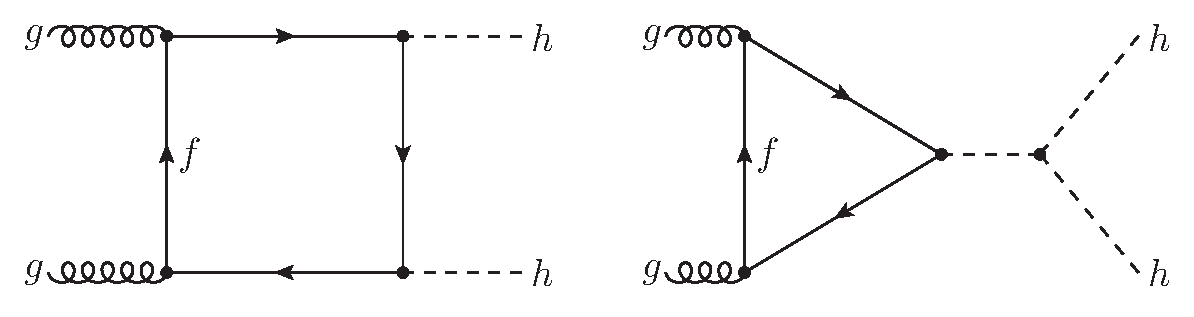
\includegraphics[width=0.90\textwidth]{plots/hhFeyn.pdf}
  \caption{\small Representative Feynman diagrams
    for Higgs pair production in gluon fusion at
    leading order.
    %
    Only the quark triangle diagram (left) is sensitive to the Higgs trilinear coupling
    $\lambda$.
    %
    In the SM, the fermion loops are dominated by the top quark contribution.
}
\label{fig:hhFeyn}
\end{center}
\end{figure}
%%%%%%%%%%%%%%%%%%%%%%%

Higgs pair production is simulated at leading order using
{\tt MadGraph5\_aMC@NLO}~\cite{Alwall:2014hca}.
%
We use a tailored {\tt MadGraph5\_aMC@NLO} model~\cite{Maltoni:2014eza} that simulates
gluon-gluon-fusion Higgs boson pair production including the effects
of the
exact form factors for the top triangle and box loops at leading
order, the latter taken from from~\cite{Plehn:1996wb}.\footnote{We note that
  since recently it is possible to compute also
  loop-induced processes in {\tt MadGraph5\_aMC@NLO} without the need of
  using specific
models~\cite{Hirschi:2015iia}.}
%
We use the default settings of the renormalization and factorization
scale of the model.
%
The Higgs boson parameters are also the same as in the default model,
in particular we use $m_h=125$ GeV, consistent with the latest
measurements from ATLAS and CMS~\cite{Aad:2014aba,Khachatryan:2014jba}.
%
The value of the Higgs trilinear coupling $\lambda$ is set to its
Standard Model value, $\lambda=m_h^2/2v^2$, with $m_h=125$ GeV
the Higgs boson mass and $v\simeq 246$ GeV the Higgs vacuum expectation
value (vev).
%
The calculation is performed in the
$n_f$=4 scheme and thus
takes into account the finite mass of the $b$-quarks.
%
For the input parton distribution functions, we 
adopt the NNPDF 3.0 $n_f = 4$ LO set~\cite{Ball:2014uwa} with
$\alpha_s(m_Z^2)=0.118$
interfaced via {\tt LHAPDF6}~\cite{Buckley:2014ana}.

In Fig.~\ref{fig:hhFeyn} we show representative Feynman diagrams
    for Higgs pair production in gluon fusion at
    leading order.
    %
    The non-trivial interplay between the diagram with a heavy quark box
    and that of the triangle, that can lead to constructive or destructive interference,
    complicates the extraction of
    the trilinear coupling
    $\lambda$ from the measurement of the Higgs pair
    production cross-section.
    %
    Higher order corrections are dominated by gluon radiation
    from either the initial state gluons or from the heavy quark loops.

    The total inclusive cross-section for this processes is
    known up to NNLO~\cite{deFlorian:2013jea}.
    %
Resummed NNLO+NNLL calculations for Higgs pair production have become available recently~\cite{deFlorian:2015moa},
leading to a moderate enhancement of the order of
few percent as compared to the fixed-order NNLO calculation.
%
Therefore, to achieve the correct higher-order value of the  integrated cross-section, we rescale our LO signal sample to match the
NNLO+NNLL
inclusive cross-section.
%
This corresponds to using a $K$-factor $\sigma_{\rm NNLO+NNLL}/\sigma_{\rm LO}=2.4$, as indicated
in Table~\ref{tab:samples}.
%
Parton level signal events are then showered with the {\tt Pythia8} Monte
Carlo~\cite{Sjostrand:2007gs,Sjostrand:2014zea} version {\tt v8.201}.
%
We use the default settings for the modeling
of the underlying event (UE), multiple parton
interactions (MPI) and pile-up, by means
of the the Monash 2013 tune~\cite{Skands:2014pea},
with the NNPDF2.3LO PDF set~\cite{Ball:2012cx}.
%


\subsection{Backgrounds: QCD multijet and $t\bar{t}$ production}

Now we turn to discuss the Monte Carlo generation of the relevant background processes.
%
All background samples are generated at leading-order
with the {\tt SHERPA} event generator~\cite{Gleisberg:2008ta}, {\tt v2.1.1}.
%
As in the case of the signal generation,
the NNPDF 3.0 $n_f = 4$ LO set with strong coupling
$\alpha_s(m_Z^2)=0.118$ is used for all samples.
%
Factorisation and renormalisation scales are set as $\mu_F=\mu_R=H_T/2$ for all
the background processes.

We consider the most relevant background
processes that contribute to the identification of
 $hh\to 4b$ candidate events.
%
This includes  QCD $4b$ multi-jet production, as well as
QCD $2b2j$ and $4j$ multi-jet samples.
%
The latter can lead to the event being identified
as signal in the case of light or charm
jets being mistagged as $b$-jets.
%
While the light jet mistag probability is small, we find that
in general the $2b2j$ and $4j$ backgrounds cannot be neglected because
of their large cross-sections and enhancement from combinatorics, that
increase their contribution as compared to a naive estimate.
%
In addition, we find that there is an important contribution from the radiation
of $b$-quarks off light partons during the parton shower, which enhances the contribution
of parton-level $2b2j$ and $4j$ events being tagged as signal events.
%

In addition to the QCD multijet processes,
we also generate $t\bar{t}$ samples
in the fully hadronic final state, which lead to a
$2b4j$ signature that can
contribute due to light jet mistags.
%
This background processes leads a similar topology that
the corresponding QCD sample.
%
Leptonic decays of top quarks can be removed by requiring
a lepton veto, and thus are not included here.
%
Single Higgs production processes, such as $Z(\to b\bar{b})h(\to b\bar{b})$
and $t\bar{t}h(\to b\bar{b})$, and electroweak backgrounds, such $Z(\to b\bar{b})b\bar{b}$,
are much smaller than the QCD backgrounds~\cite{Wardrope:2014kya,deLima:2014dta}
and thus not included in the present analysis.
%



The LO cross-sections for
the background samples have been rescaled so that the integrated
distributions reproduce known higher-order QCD results.
%
For the $4b$ and $2b2j$ samples, a NLO/LO $K$-factor has been determined
using {\tt MadGraph5\_aMC@NLO}~\cite{Alwall:2014hca}, which turns out to be 1.6 and 1.3
respectively.
%
For the $4j$ sample, we rescale it using the {\tt BLACKHAT}~\cite{Bern:2011ep}
results, that indicate
a NLO/LO $K$-factor of 0.6.
%
Finally, the LO cross-section for $t\bar{t}$ production has been rescaled
to match the NNLO+NNLL calculation of Ref.~\cite{Czakon:2013goa}, which leads
to a $K$-factor of 1.4.
%
The $K$-factors that we use to rescale all the background samples have been collected in
Table~\ref{tab:samples}.


At the generation level, the following loose selection 
cuts are applied to
background events.
%
Each final state particle in the hard process must have $p_T \ge 20$ GeV, and be located
in the central  rapidity
region with
$| \eta | \le 3.0$.
%
In addition, at the matrix-element level
all final state particles must be separated by a minimum $\Delta R_{\mathrm{min}} =0.1$.
%
We have checked that the generator-level cuts are loose enough to have
no influence over the analysis cuts.
%


The LO cross-sections,
number of generated events and the higher-order $K$-factors
applied to the signal and background
samples are collected in Table~\ref{tab:samples}.
%
We see that the $t\bar{t}$ and QCD $4b$ samples are of
the same order of magnitude, however, the former can be efficiently
reduced by using top quark reconstruction criteria.
%
The $bbjj$ cross-section is more than two orders
of magnitude larger as compared to the
$4b$ result, however, as we will show,
due both to combinatorics and to $b$-quark radiation
during the parton shower it can be comparable or larger
than the irreducible QCD background.
%
 For top quark production, only the hadronic final state is generated.
 %
 
 


 %%%%%%%%%%%%%%%%%%%%%%%%%%%%%%%%%%%%%%%%%%%%%%%%%%%%%%%%%%%%%%%
 %%%%%%%%%%%%%%%%%%%%%%%%%%%%%%%%%%%%%%%%%%%%%%%%%%%%%%%%%%%%%%%
\begin{table}[h]
  \small
\begin{center}
\begin{tabular}{|c|c|c|c|c|c|}
\hline
Process &  Generator & $N_{\mathrm{evt}}$ & $\sigma_{\mathrm{LO}}$ (pb)  & $K$-factor \\
\hline
\hline
$pp \to hh$ &  {\tt MadGraph5\_aMC@NLO} & 100K & $1.71\times10^{-2}$  &  2.4  (NNLO+NNLL~\cite{deFlorian:2013jea,deFlorian:2015moa}) \\
\hline
\hline
$pp \to b\bar{b}b\bar{b}$ &  {\tt SHERPA}v2.1.1 & 3M &$1.12 \times10^3$  & 1.6 (NLO~\cite{Alwall:2014hca}) \\
$pp \to b\bar{b}jj$ &  {\tt SHERPA}v2.1.1 & 3M & $2.66 \times 10^5$ & 1.3 (NLO~\cite{Alwall:2014hca}) \\
$pp \to jjjj$ &  {\tt SHERPA}v2.1.1 & 3M  & $9.71\times 10^6$ &  0.6 (NLO~\cite{Bern:2011ep})\\
$pp \to t\bar{t}\to b\bar{b}jjjj$ &  {\tt SHERPA}v2.1.1 & 3M & $2.51\times 10^3$   & 1.4 (NNLO+NNLL~\cite{Czakon:2013goa})\\
\hline
\end{tabular}
\caption{\small Details of the signal and background Monte
  Carlo samples generated,
  together with the corresponding generator-level LO cross-sections.
  %
  For top quark production, only the hadronic final state is generated.
  %
We also provide in each case the corresponding inclusive $K$-factor
  that is applied in each case to correctly normalize the distribution to the known
  higher-order results. \label{tab:samples}
} 
\end{center}
\end{table}%
%%%%%%%%%%%%%%%%%%%%%%%%%%%%%%%%%%%%%%%%%%%
%%%%%%%%%%%%%%%%%%%%%%%%%%%%%%%%%%%%%%%%%%%%%%%%%%%%%%%%%%%%%%%

As a cross-check of the {\tt SHERPA}
background cross-sections reported in Table~\ref{tab:samples}, we have produced leading-order
multi-jet samples
using {\tt MadGraph5\_aMC@NLO}, and
benchmarked them with the results for the same processes reported in
Ref.~\cite{Alwall:2014hca}.
%
For comparison with the latter numbers, 
we require in all samples four anti-$k_T$ $R=0.5$ jets with $p_T \ge 80 $ GeV, and the leading jet must have $p_T \ge 100$ GeV, and
also that all jets must be within an acceptance of $|\eta| \le 2.5 $.
%
We find good agreement, within the scale uncertainties, between the {\tt MadGraph5\_aMC@NLO} and {\tt SHERPA} calculations of the multi-jet
backgrounds.


\subsection{Modelling of detector resolution}

While it is beyond the scope of this work to perform a full
detector simulation, it is still important to include an estimate of detector
effects in the analysis, in particular for the finite resolution
in energy and momentum, which will affect some kinematical variables, in particular
the invariant mass of the Higgs candidates.
%
For example, in the absence of any four-momentum smearing, the impact of the $m_h$
distributions of the Higgs candidates in the MVA
would be unrealistically large.

In this work, we simulate the finite energy resolution of the ATLAS and CMS
hadronic calorimeters by applying a Gaussian smearing of the transverse
momentum $p_T$ of all
final-state particles, before jet clustering,
with mean zero and standard deviation $\sigma_E$, that is
%
\be
\label{eq:smearing}
p_T^{(i)} \, \to \, p_T^{(i)\prime}= \lp 1+ r_i\cdot\sigma_E \rp\, p_T^{(i)} \, , \quad
i=1,\ldots,N_{\rm part} \, ,
\ee
with $r_i$ an univariate Gaussian random number, different for each
of the $N_{\rm part}$ particles in the event.
%
We take as baseline value a momentum smearing
factor of $\sigma_E=5\%$.
%


To account for the finite angular resolution of the calorimeter,
the $\eta$-$\phi$ plane is divided into regions of
$\Delta \eta \times \Delta \phi=0.1$, and each final state particle
which falls in each of these cells is set of have the same $\eta$
and $\phi$ values of the center of the cell.
%
Finally, the particle's energy is recalculated from the smeared $p_T^\prime$,
$\eta^\prime$ and $\phi^\prime$ values to satisfy the mass-shell
condition.


Our modelling of detector simulation has been motivated
to lead to a mass resolution of
reconstructed Higgs candidates of around 10 GeV, consistent
with the hadronic mass resolutions of ATLAS and CMS.
%
In  Fig.~\ref{fig:higgs-mass-resolution} we show the
invariant mass distributions of the leading
Higgs candidate in signal events for the
resolved category (see Sects.~\ref{sec:analysis}
and~\ref{sec:results}), together with
a Gaussian fit,
used to determine the mass resolution.
%
We indeed  find a mass resolution of about 8\%, corresponding
    to around 10 GeV for $m_H=125$ GeV.
%
    For completeness, in Fig.~\ref{fig:higgs-mass-resolution}
    we also show the corresponding
    mass distributions of Higgs candidates
    in the case of $\la n_{\rm PU}\ra=80$ PU events
    subtracted with {\tt SoftKiller} (see Sect.~\ref{sec:pileup}).
    %
    In the case of PU, the mass resolution is degraded down to
    around 11\%, corresponding to 
    14 GeV.
    %
        
%%%%%%%%%%%%%%%%%%%%%%%%
\begin{figure}[t]
  \begin{center}
    \vspace{-1cm}
  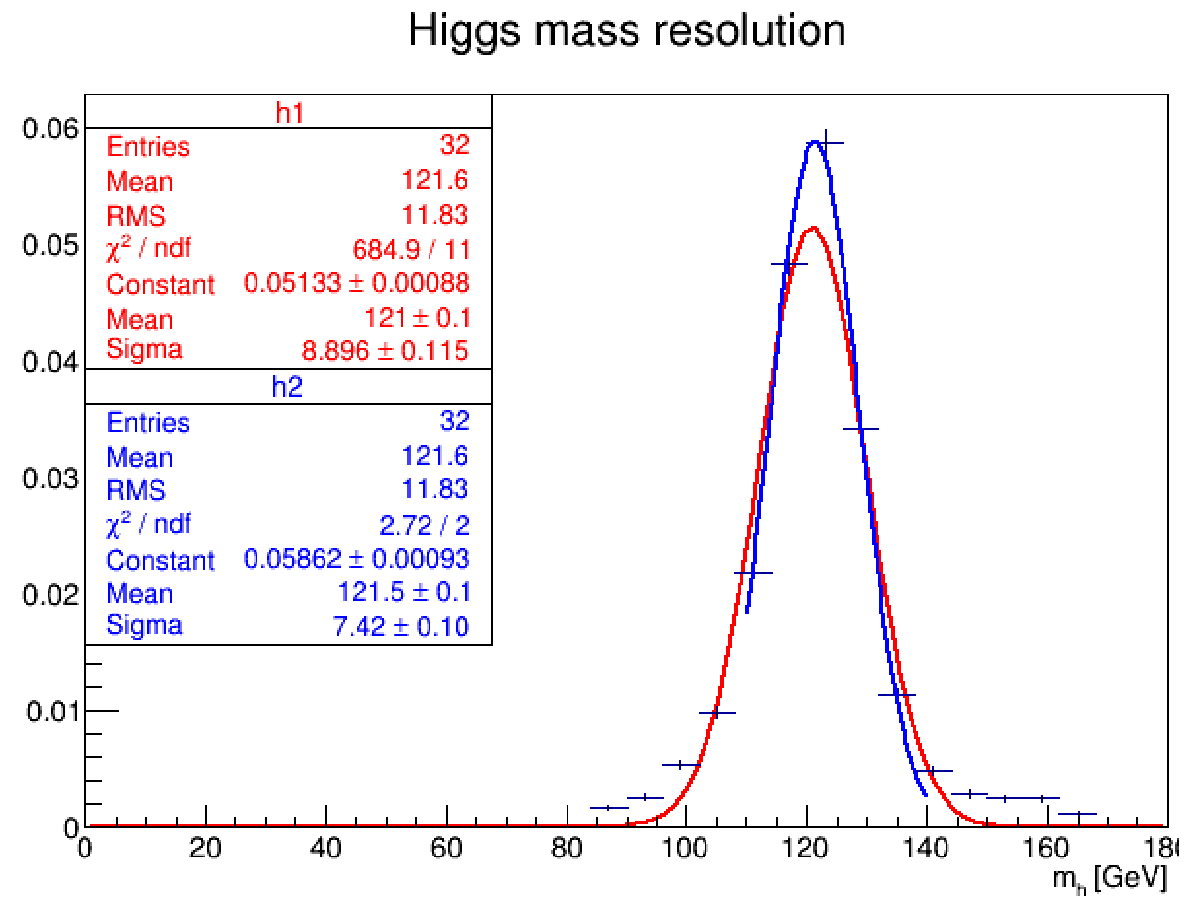
\includegraphics[width=0.49\textwidth]{plots/higgs_mass_res_noPU.pdf}
  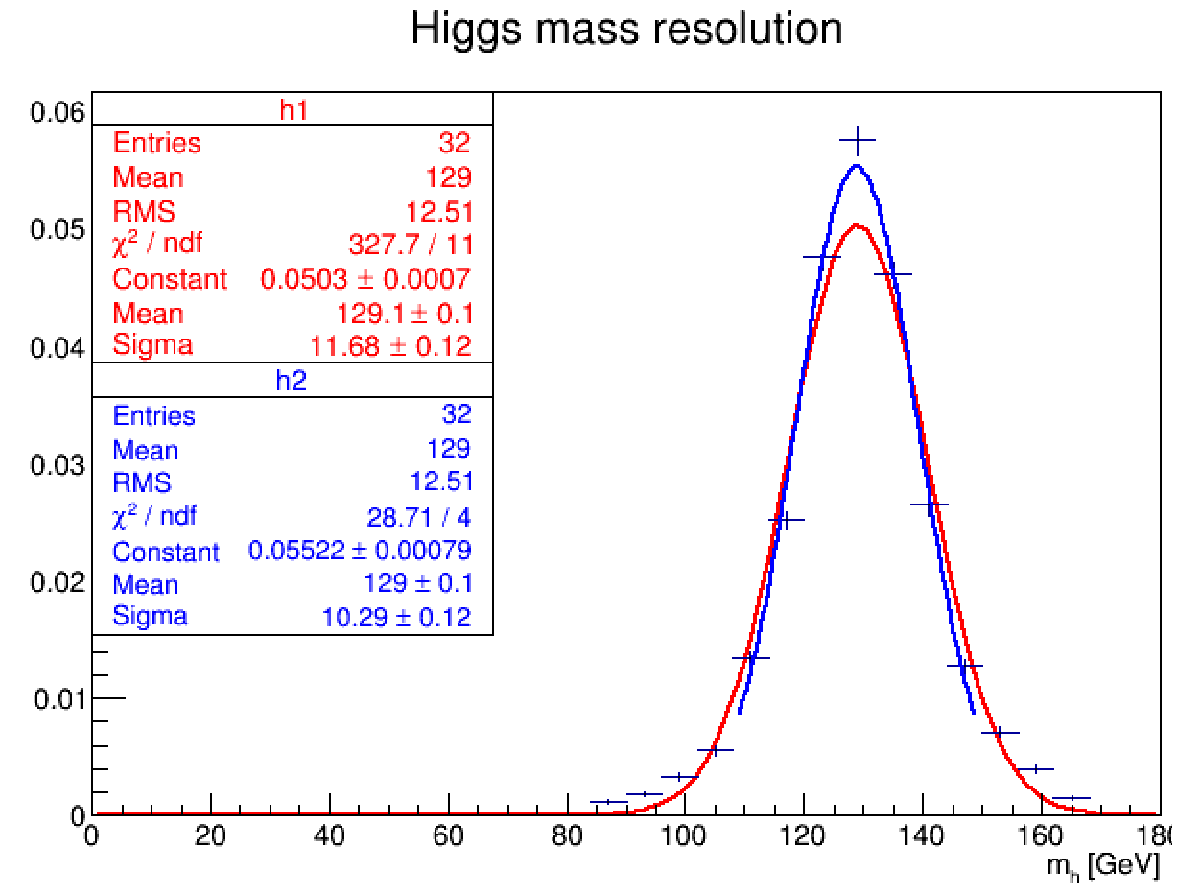
\includegraphics[width=0.49\textwidth]{plots/higgs_mass_res_PU80.pdf}
  \caption{\small The invariant mass distributions of the leading
    Higgs candidates in signal events for the resolved category, without
    PU (left plot) and with PU (right plot),
    together with Gaussian fits  used to determine the mass resolution.
    %
    In the latter case, $\la n_{\rm PU}\ra=80$, with {\tt SoftKiller}
     used for PU subtraction.
}
\label{fig:higgs-mass-resolution}
\end{center}
\end{figure}
%%%%%%%%%%%%%%%%%%%%%%%




%%%%%%%%%%%%%%%%%%%%%%%%%%%%%%%%%%%%%%%%%%%%%%%%%%%%


\section{Analysis strategy}
\label{sec:analysis}

In this section we describe our analysis strategy.
%
First of all, we discuss the settings
for jet clustering  and the strategy for $b$-tagging.
%
Then we discuss the categorisation of events in different
topologies and how to prioritise among them.
%
We motivate our choice of analysis cuts by comparing signal and background
for representative kinematical distributions.
%
Finally, we describe the simulation of PU and validate
the PU subtraction strategy that we adopt.

\subsection{Jet reconstruction}

After the  parton shower, final state particles
are clustered using the
jet reconstruction algorithms
obtained from
{\tt FastJet}~\cite{Cacciari:2011ma,Cacciari:2005hq},
{\tt v3.1.0}.
%
We use different types of jet definitions:
\begin{itemize}
\item {\it Small-$R$ jets}.

  These are jets  reconstructed with the
  anti-$k_T$ clustering algorithm~\cite{Cacciari:2008gp} with $R=0.4$ radius.
  %
  These small-$R$ jets are required
  to have transverse momentum $p_T \ge 40$~GeV
  and pseudo-rapidity $|\eta|<2.5$, within the central 
  acceptance of ATLAS and CMS, the region
  where $b$-tagging is possible.

\item {\it Large-$R$ jets}.

  These jets are also constructed with the
  anti-$k_T$ clustering algorithm, now using a $R=1.2$ radius.
  %
  Large-$R$ jets are required to have
  $p_T \ge 200$~GeV and lie in a pseudo-rapidity region of
  $|\eta|<2.0$.
  %
  The more restrictive range  in pseudo-rapidity
  as compared to the small-$R$ jets
  is motivated by mimicking the  experimental requirements
  in ATLAS and CMS
  related to the track-jet based calibration~\cite{Aad:2014bia,ATLAS:2012kla}.

  In addition to the basic $p_T$ and $\eta$
  acceptance requirements, large-$R$ jets should also
  satisfy the  BDRS mass-drop tagger (MDT)~\cite{Butterworth:2008iy}
  conditions.
  %
  We use the {\tt FastJet} default
  parameters of  $\mu = 0.67$ and $y_{\textrm{cut}}= 0.09$.
  %
  Before applying the MDT, the large-$R$ jet
  constituents are reclustered with the Cambridge/Aachen (C/A)
  algorithm~\cite{Dokshitzer:1997in,Wobisch:1998wt}
  with $R=1.2$.

  
\item {\it Small-$R$ subjets}.

  These subjets are constructed by reclustering the constituents
  of a large-$R$ jet, again with the
  anti-$k_T$ algorithm,
  but this time with a smaller radius parameter, namely
  $R=0.3$~\cite{Aad:2015uka}.
 %
  These small-$R$ subjets will be the main input for
  $b$-tagging in the boosted category.
  %
  They are required to satisfy $p_T > 50$~GeV and $|\eta|<2.5$.
  %
\end{itemize}

In addition, we have
also explored the possible improvements
in the analysis from the use
of variable-$R$ jets~\cite{Krohn:2009zg}, finding
a similar performance as in the case of fixed-$R$ jets.
%
This is explained by the fact that
variable-$R$ jets are more suitable when
the degree of boost of the final state being reconstructed can
differ substantially~\cite{Cacciari:2008gd},
such as in heavy resonance
searches~\cite{Aad:2015fna},
where the degree of boost of the final state
is {\it a priori} unknown.


For the   boosted and intermediate categories,
which involve the use of large-$R$ jets,
we use jet substructure variables~\cite{Salam:2009jx,Aad:2013gja} to
improve the significance of the discrimination between signal and background
events in the MVA.
%
In particular we  consider the following jet
substructure variables:
\begin{itemize}
\item The $k_T$-splitting scale~\cite{Butterworth:2002tt,Butterworth:2008iy}.

  This variable is defined by reclustering the constituents of a jet with the
  $k_t$ algorithm~\cite{Ellis:1993tq},
  which usually clusters last the harder constituents, and then
  taking the $k_t$ distance measure between the two subjets at the final stage of the recombination
  procedure,
  \be
  \label{eq:ktsplitting}
\sqrt{d_{12}} \equiv {\rm min}\lp p_{T,1},p_{T,2}\rp \cdot \Delta R_{12} \, .
\ee
with $p_{T,1}$ and $p_{T,2}$ the transverse momenta of the two subjets merged
in the final step of the clustering, and $\Delta R_{12}$ the corresponding
angular separation.
  
\item The ratio of 2-to-1 subjettiness $\tau_{12}$~\cite{Thaler:2010tr,Thaler:2011gf}.

  The $N$-subjettiness variables $\tau_N$ are defined by clustering the constituents
  of a jet with the exclusive $k_t$ algorithm~\cite{Catani:1993hr}
  and requiring that $N$ subjets are found,
  \be
  \tau_N \equiv \frac{1}{d_0} \sum_k p_{T,k}\cdot {\rm min}\lp \delta R_{1k}, \ldots,
  \delta R_{Nk}\rp \, , \qquad d_0\equiv \sum_k p_{T,k}\cdot R \, ,
  \ee
  with $p_{T,k}$ is the $p_T$ of the constituent particle $k$ and $\delta R_{ik}$ the distance from
  subjet $i$ to constituent $k$.
  %
  In this work we use as input to the MVA the ratio of 2-subjettiness to 1-subjettiness
  \be
  \label{eq:tau21}
\tau_{21} \equiv \frac{\tau_2}{\tau_1} \, ,
  \ee
  which provides good discrimination 
  between QCD jets and jets arising from the decay of
  a heavy resonance.
  
\item The ratios of energy correlation functions (ECFs)  $C^{(\beta)}_2$~\cite{Larkoski:2013eya} and
  $D_2^{(\beta)}$~\cite{Larkoski:2014gra}.

  The ratio of energy correlation functions $C_2^{(\beta)}$ is defined as
  \be
  \label{eq:c2}
C_2^{(\beta)} \equiv \frac{ {\rm ECF}(3,\beta) {\rm ECF}(1,\beta)}{\lc {\rm ECF}(2,\beta)\rc ^2} \, ,
\ee
while $D_2^{(\beta)}$ is instead defined as a double ratio of ECFs, that is
\be
e_3^{(\beta)}\equiv \frac{ {\rm ECF}(3,\beta)}{\lc {\rm ECF}(1,\beta)\rc^3} \, , \quad
  e_2^{(\beta)}\equiv \frac{ {\rm ECF}(2,\beta)}{\lc {\rm ECF}(1,\beta)\rc^2} \, , \quad
  \label{eq:d2}
D_2^{(\beta)} \equiv \frac{ e_3^{(\beta)})}{\lp e_2^{(\beta)} \rp^3} \, .
\ee
The energy correlation functions ${\rm ECF}(N,\beta)$ are defined
  in~\cite{Larkoski:2013eya} with the motivation that $(N+1)$-point correlators
  are sensitive to $N$-prong substructure.
  %
  The free parameter $\beta$ is set to a value of $\beta=2$,
  as recommended by the authors of Refs.~\cite{Larkoski:2013eya,Larkoski:2014gra}.
\end{itemize}



\subsection{Tagging of $b$-jets}
\label{sec:btagging}

In this analysis we adopt
a $b$-tagging strategy along the lines
of current ATLAS performance~\cite{Aad:2013gja,Aad:2015ydr},
though differences with respect to
the corresponding CMS
settings~\cite{Khachatryan:2011wq,Chatrchyan:2012jua}
do not modify qualitatively our results.
%
For each type of jet definition used, a different
$b$-tagging strategy is adopted:

\begin{itemize}

\item {\it Small-$R$ jets}.

  %
  If a small-$R$ jet has at least one $b$-quark among their constituents,
  it will be tagged as a $b$-jet with probability $f_b$.
  %
  In order to be considered in the $b$-tagging algorithm,
  $b$-quarks inside the small-$R$ jet
  should satisfy $p_T \ge 15$ GeV~\cite{Aad:2015ydr}.
  %
  The probability of tagging a jet is not modified
  if more than one $b$-quark is found among the jet constituents.


  
  If no $b$-quarks are found among the constituents
  of this jet, it can be still be tagged as a $b$-jet with
  a mistag rate of $f_l$, unless a charm quark is present instead,
  and in this case the mistag rate is $f_c$.
  %
  Only jets that contain at least one (light or charm)
  constituent
  with $p_T \ge 15$ GeV can induce a fake $b$-tag.

  
  We attempt to $b$-tag only the four (two) hardest small-$R$ jets
  in the resolved (intermediate) category.
  %
  Trying to $b$-tag all the
  small-$R$ jets that satisfy the acceptance cuts worsens the
  overall performance
  due to combinatorics.

  \item {\it Large-$R$ jets}.

    Large-$R$ jets are $b$-tagged by
    ghost-associating anti-$k_T$ $R=0.3$ (AKT03)
    subjets to the original large-$R$
    jets~\cite{Cacciari:2007fd,Aad:2013gja,
      ATLAS-CONF-2014-004,Aad:2015uka}.
    %
    A large-$R$ jet is considered $b$-tagged if both
    the leading and subleading AK03 subjets, where the ordering
    is done in the subjet $p_T$, are both individually $b$-tagged,
    with the same criteria as the small-$R$ jets.
    %
     Therefore, a large-$R$ jet where the two leading
    subjets have at least one $b$-quark will be tagged
    with probability $f_b^2$.
    
    As in the case
    of small-$R$ jets, we only attempt to $b$-tag the two leading subjets,
    else one finds a degradation of the
    signal significance due to combinatorics.
    %
    The treatment of the $b$-jet mis-identification
    from light and charm jets
    is the same as for the small-$R$ jets.
  
\end{itemize}

Concerning the values of the $b$-tag probability, $f_b$, and
the $b$-mistag probability of light and charm jets, $f_l$ and  $f_c$
respectively,
we used the values $f_b=0.8$, $f_l=0.01$
and  $f_c=0.1$.





\subsection{Event categorisation}
\label{sec:categorisation}

The present analysis follows a strategy similar to the
scale-invariant resonance tagging of Ref.~\cite{Gouzevitch:2013qca}.
%
Rather than restricting to a specific event topology,
we aim to consistently combine the information from
the three possible topologies: boosted, intermediate and
resolved, with the optimal cuts for each category being determined
separately.
%
This approach is robust
under variations of
the underlying production model of Higgs pairs is modified,
for instance in the case of
BSM dynamics, which can substantially increase
the degree of boost of the final state.


The three categories are defined as follows:
\begin{itemize}
\item {\it Boosted category}.

  An event which
  contains at least two large-$R$ jets, with the two leading jets
 being $b$-tagged.
 %
 Each of these two large-$R$, $b$-tagged, jets are 
 thus candidates
 to contain the decay products of a Higgs boson.

\item {\it Intermediate category}.

  An event with exactly one large-$R$, $b$-tagged, jet, which
  is assigned to be the leading Higgs candidate.
  %
  In addition, we require at least two small-$R$, $b$-tagged, jets,
  which must be separated with respect to the large-$R$ jet
  by an angular distance of $\Delta R\ge 1.2$.
  %
    
  The subleading Higgs boson candidate is reconstructed
  by selecting the two $b$-tagged small-$R$ jets that minimize the difference
  between the invariant mass of the large-$R$ jet
  with that of the dijet obtained
  from the sum of the two small-$R$ jets.
  
\item {\it Resolved category}.

  
 An event with at least
  four $b$-tagged small-$R$ jets.
  %
  The two Higgs candidates are reconstructed out of the
  leading four small-$R$ jets in the event
  by considering all possibilities of forming two pairs of jets
  and then choosing the configuration that minimizes the relative difference of
  dijet masses.
  %
  
\end{itemize}


Once a Higgs boson candidate has been identified,
its invariant mass is required to lie within a fixed window
around the nominal Higgs boson mass of $m_h= 125$
GeV.
%
In particular we require the condition
\be
\label{higgsmasswindow}
|m_{h,j} - 125| < 40~{\rm GeV} \, ,\, j=1,2 \, ,
\ee
where $m_{h,j}$ is the invariant mass of each of the two reconstructed  Higgs candidates.
%
This cut is substantially looser than the corresponding
cut used in the typical ATLAS and CMS $h\to b\bar{b}$
analyses~\cite{Aad:2012gxa,Chatrchyan:2013zna}.
%
The motivation
for this choice 
is that further improvements of the
signal significance will be obtained using an MVA.
%
Only events where the two Higgs candidates satisfy
Eq.~(\ref{higgsmasswindow}) are classified as signal events.
%

These three categories are not exclusive:
a given event can be assigned to more than one category, for
example, satisfying the requirements of both the intermediate
and resolved
categories at the same time.
%
The exception is the boosted and intermediate categories, which have
orthogonal jet selection requirements.
%
The optimization of the analysis
of the three categories is performed inclusively, and
then events are exclusively assigned to specific category
starting with the one with the highest signal significance.


The separate optimisation of the three categories needs to be performed in
a inclusive analysis, and then we introduce a
 priorisation starting with the category of highest signal significance.


 This has been achieved as follows.
 %
First of all we perform an inclusive analysis, and optimise the
signal significance
$S/\sqrt{B}$ in each of the three categories separately, including
the MVA.
%
We find that the category with higher significance is
the boosted one,
followed by the intermediate and the resolved ones, the latter two
with similar significance.
%
Therefore, for the final analysis, we turn to an exclusive approach:
if an event satisfies the boosted requirements, it is assigned to
this category, else we check if it suits the intermediate
requirements.
%
It the event also fails the intermediate category
requirements, we
then check if it pass the resolved selection criteria.
%
The resulting exclusive event samples are then separately processed
through the MVA, allowing a consistent combination
of the significance of the three event categories.

\subsection{Motivation for basic kinematic cuts}

We now motivate the values of
kinematic cuts applied to the different categories, 
comparing representative kinematic distributions between
signal and background events.
%
We first present results without PU, and then
discuss
the impact of PU
on the description of the various kinematic
distributions.
%
In the following, all
distributions will be normalized to their total integral.


In Fig.~\ref{fig:cutplots1} we show
the $p_T$ distributions
of the
  leading and subleading large-$R$ jets in the boosted category, comparing
  the shapes of the distribution in signal and background events.
  %
  We observe that the background distribution
falls off more rapidly as a function of $p_T$ than the di-Higgs signal.
  %
  On the other hand, the cut in $p_T$ cannot be too strong to avoid
  a substantial degradation of signal selection efficiency,
  specially taking into account the subleading large-$R$ jet.
  %
  This comparison justifies the cut of $p_T \ge 200$ GeV
  for the large-$R$ jets that we impose in the boosted category.
  

%%%%%%%%%%%%%%%%%%%%%%%%%%%%%%%%%%%%
\begin{figure}[t]
\begin{center}
 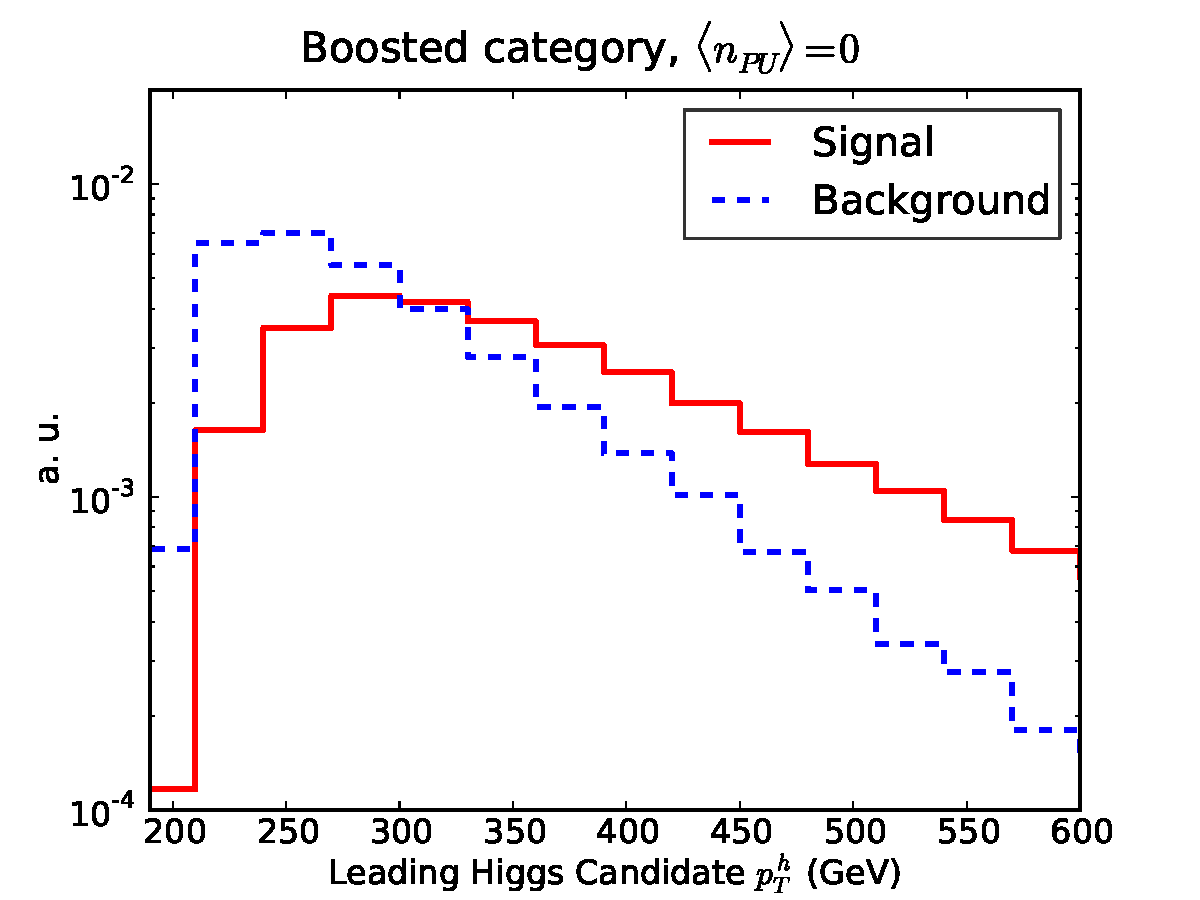
\includegraphics[width=0.48\textwidth]{plots/pt_H0_bst_C1d_noPU.pdf}
 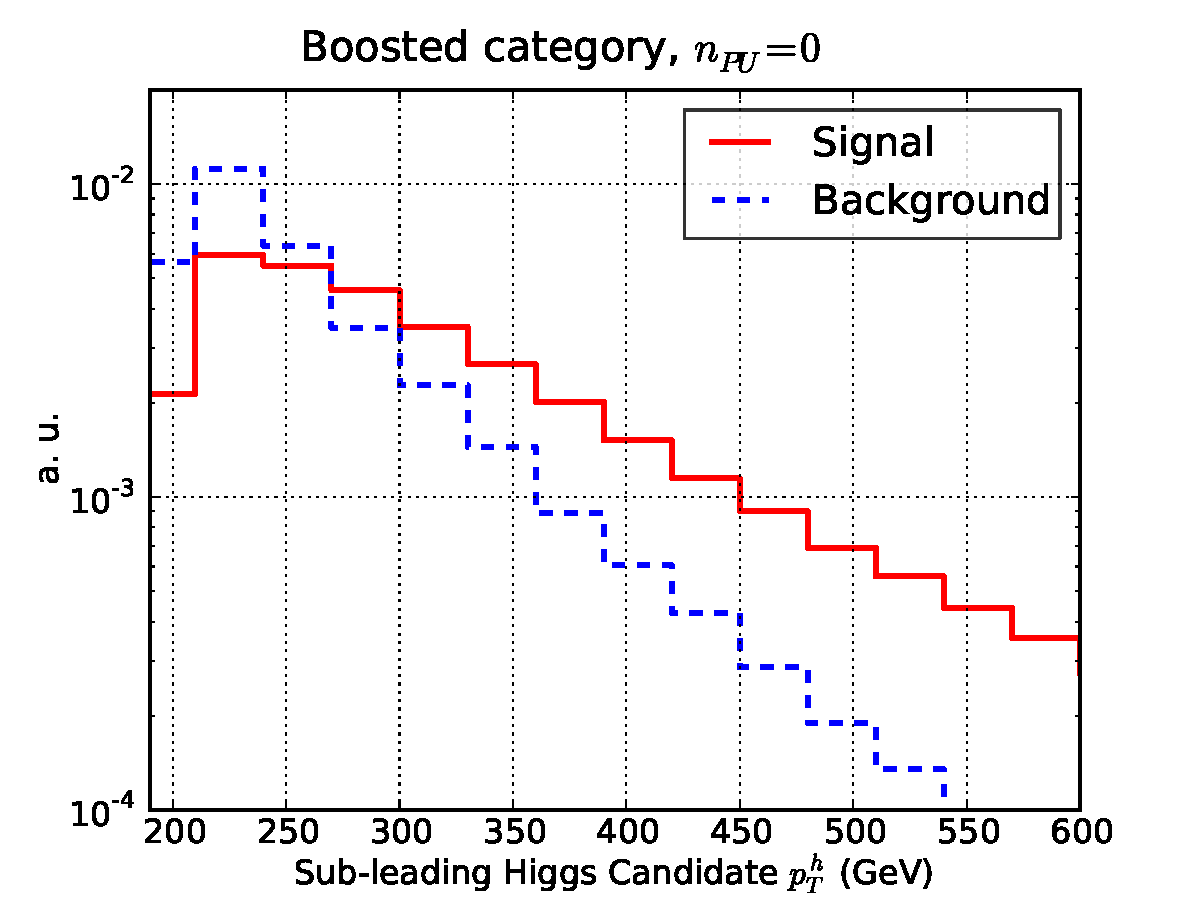
\includegraphics[width=0.48\textwidth]{plots/pt_H1_bst_C1d_noPU.pdf}
\caption{\small  Comparison of the $p_T$ distributions of the
  leading (left plot) and
  subleading (right plot) large-$R$ jets in the boosted category,
  in in signal and background events.
  %
  Distributions have been normalized to unity.
}
\label{fig:cutplots1}
\end{center}
\end{figure}
%%%%%%%%%%%%%%%%%%%%%%%


Another selection requirement for the boosted category is that the two
leading AKT03 subjets of the large-$R$ jet must be relatively hard,
in particular they should satisfy $p_T \ge $ 50 GeV.
%
To motivate this cut, in Fig.~\ref{fig:cutplots22}
we show the distribution in $p_T$ of the leading
and subleading AKT03 subjets in the subleading large-$R$ jet in events
corresponding to the boosted category.
%
It is clear from the comparison that the subjet $p_T$ spectrum is
relatively harder in the signal with respect to the background.
%
On the other hand, considering the subleading AKT03 subjet,
this cut in $p_T$
cannot be too harsh, to maintain a high signal selection
efficiency.
%
Therefore,
as for the previous distribution, also here 
a compromise between suppressing backgrounds but keeping a large fraction of
signal events is crucial.


%%%%%%%%%%%%%%%%%%%%%%%%%%%%%%%%%%%%
\begin{figure}[t]
\begin{center}
 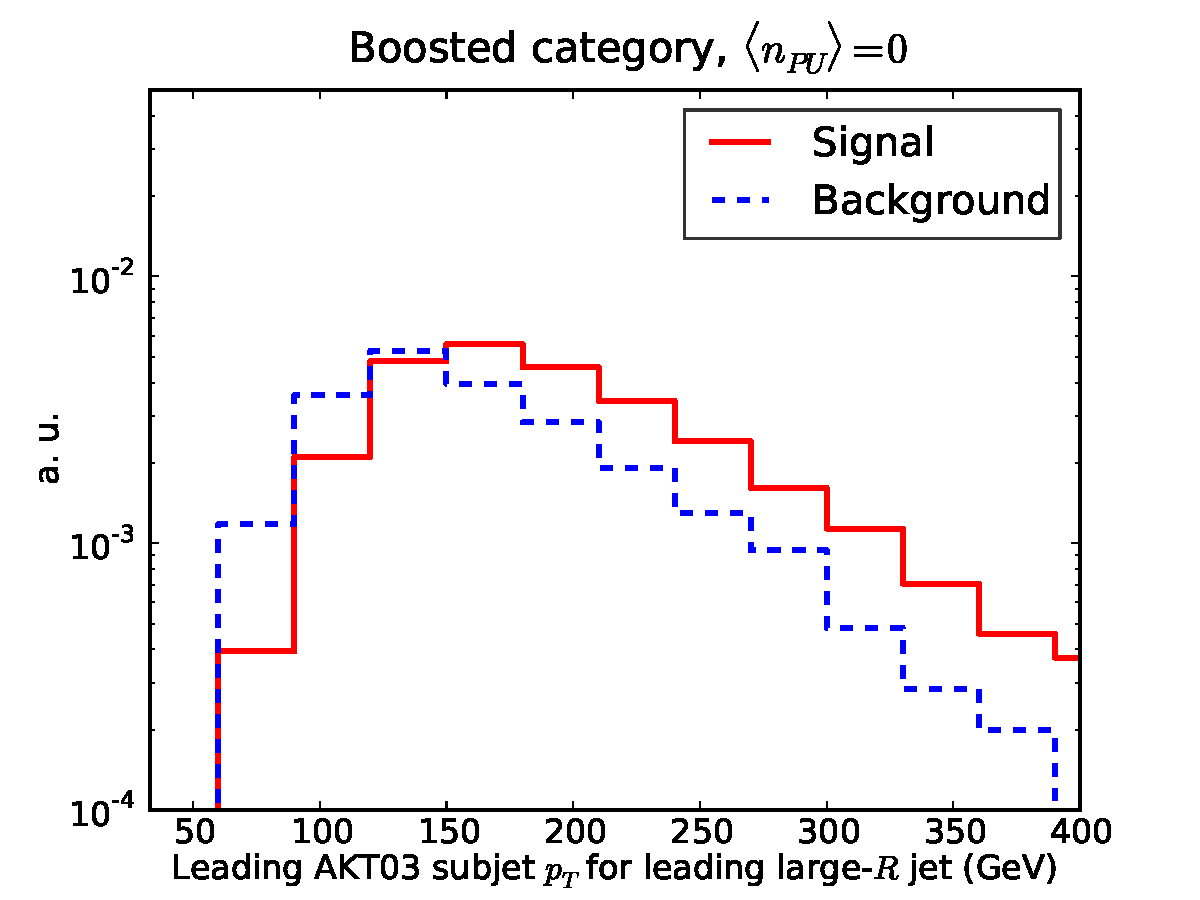
\includegraphics[width=0.48\textwidth]{plots/pt_leadSJ_fj2_noPU.pdf}
 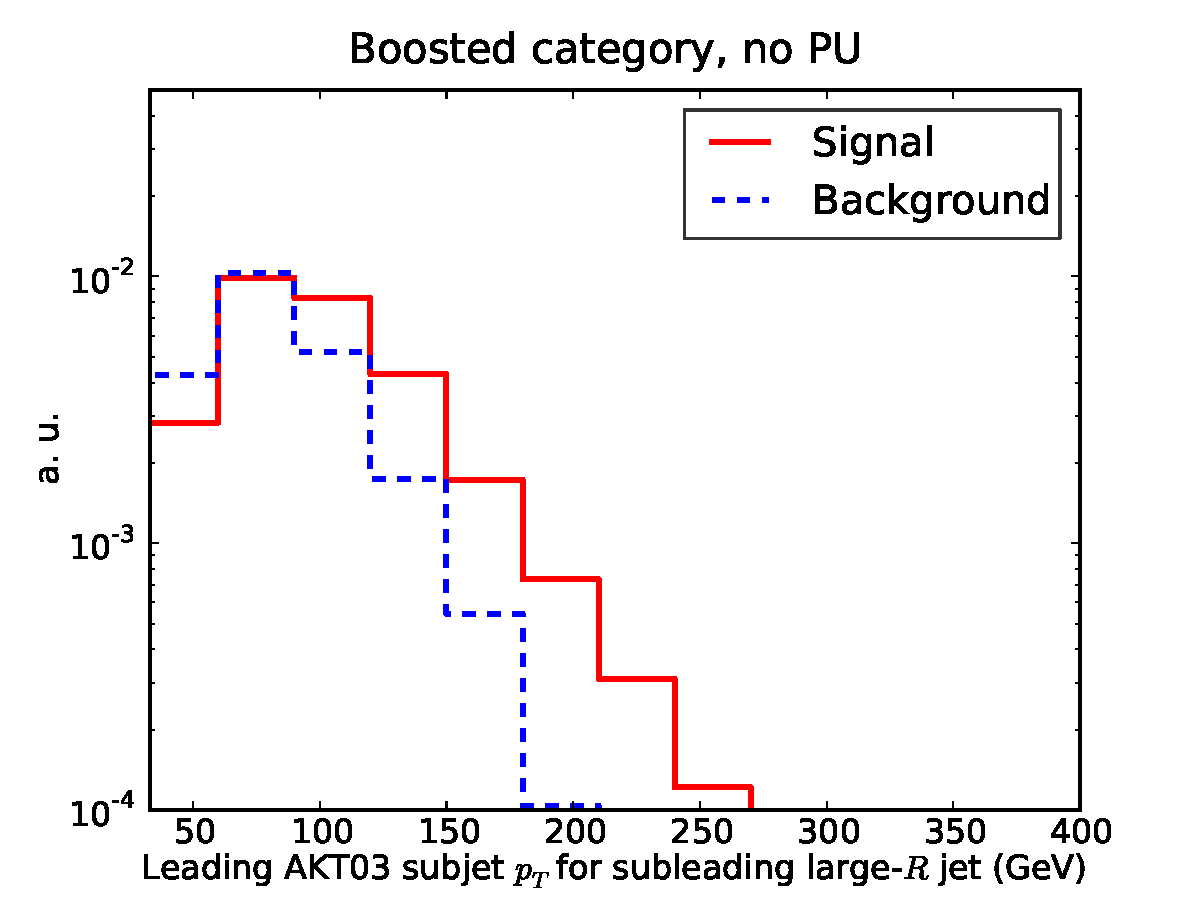
\includegraphics[width=0.48\textwidth]{plots/pt_subleadSJ_fj2_noPU.pdf}
 \caption{\small  Same as Fig.~\ref{fig:cutplots1} for the two leading AKT03
   subjets in the subleading Higgs candidate large-$R$ jet.
}
\label{fig:cutplots22}
\end{center}
\end{figure}
%%%%%%%%%%%%%%%%%%%%%%%


Turning to the resolved category, an important aspect to account
in the corresponding selection
cuts is the fact that the $p_T$ distribution
of the four leading small-$R$ jets of the event can be relatively soft,
specially for the subleading jets.
%
As noted in~\cite{deLima:2014dta}, this is a consequence of the fact
that in general the boost from the Higgs decays is moderate.
%
These considerations lead to the requirement that the $p_T$
selection
for the small-$R$ jets cannot be too large.
%
In Fig.~\ref{fig:cutplots23}
we show the distribution in $p_T$ of the four leading
small-$R$ jets in signal and background events: we observe that both
distributions are peaked at $p_T \le 50$ GeV, with the signal distribution
eventually becoming dominant at large $p_T$.
%
The feasibility to being able to trigger on four small-$R$ jets with a relatively
soft $p_T$ distribution is one of the experimental challenges for
exploiting the resolved category in this final state,
and hence the requirement that $p_T \ge 40$ GeV for
the small-$R$ jets.
%
In  Fig.~\ref{fig:cutplots23} we also show the
rapidity distribution of the the small-$R$
jets in the resolved category.
%
As expected, the production
is mostly central, more in the case
of signal events, since backgrounds are dominated by
QCD $t$-channel exchange, and thus the
selection criteria on the jet rapidity  are highly efficient.


%%%%%%%%%%%%%%%%%%%%%%%%%%%%%%%%%%%%
\begin{figure}[t]
\begin{center}
 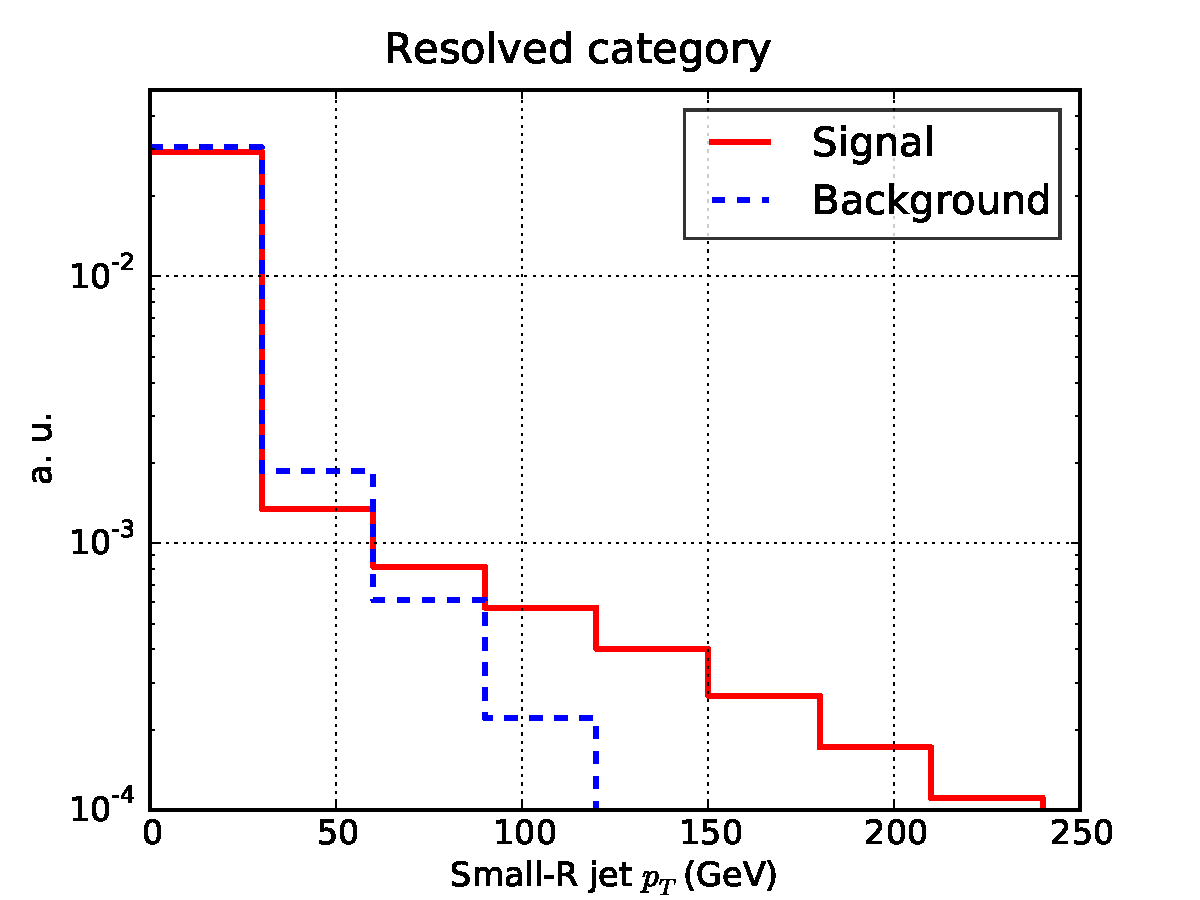
\includegraphics[width=0.48\textwidth]{plots/pt_smallRjets_res_noPU.pdf}
 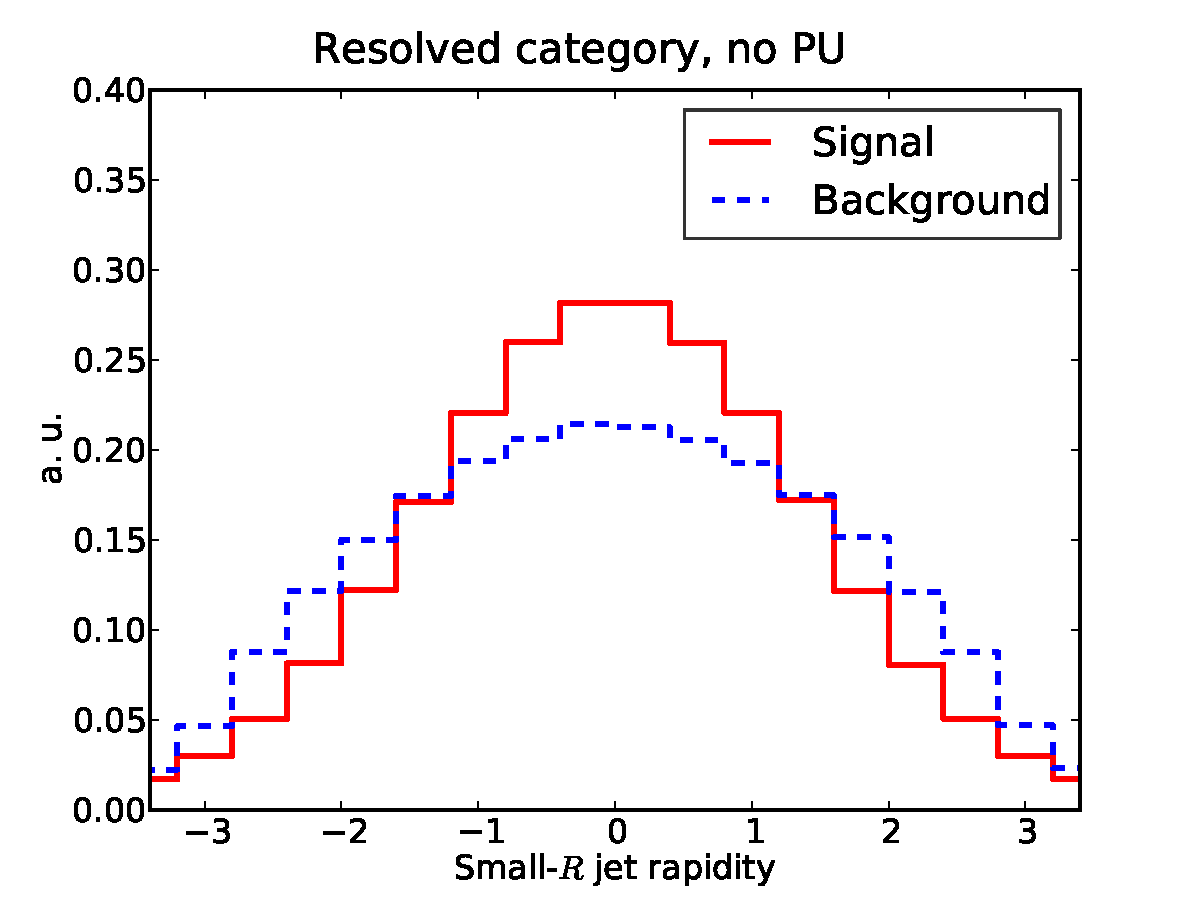
\includegraphics[width=0.48\textwidth]{plots/eta_smallRjets_res_noPU.pdf}
 \caption{\small Same as Fig.~\ref{fig:cutplots1}, now for the
   $p_T$ and rapidity distributions of the small-$R$
   jets corresponding to the resolved selection.
}
\label{fig:cutplots23}
\end{center}
\end{figure}
%%%%%%%%%%%%%%%%%%%%%%%

One of the selection cuts with highest discrimination power is the requirement
that the invariant mass of the Higgs candidate (di)jets must lie within a window
around the nominal Higgs value, Eq.~(\ref{higgsmasswindow}).
%
In Fig.~\ref{fig:mHHinv} we show the invariant mass
of the leading reconstructed Higgs candidates, before the Higgs mass window
selection
  is applied, for the resolved and boosted categories.
%
While the signal distribution is of course peaked at the
nominal Higgs mass, the background distributions
show no particular
structure.
%
The
width of the Higgs mass peak is driven both from QCD effects,
such as initial-state radiation (ISR)
and out-of-cone radiation, as well
as from the four-momenta smearing applied to final state particles.
%

%%%%%%%%%%%%%%%%%%%%%%%%%%%%
\begin{figure}[t]
\begin{center}
  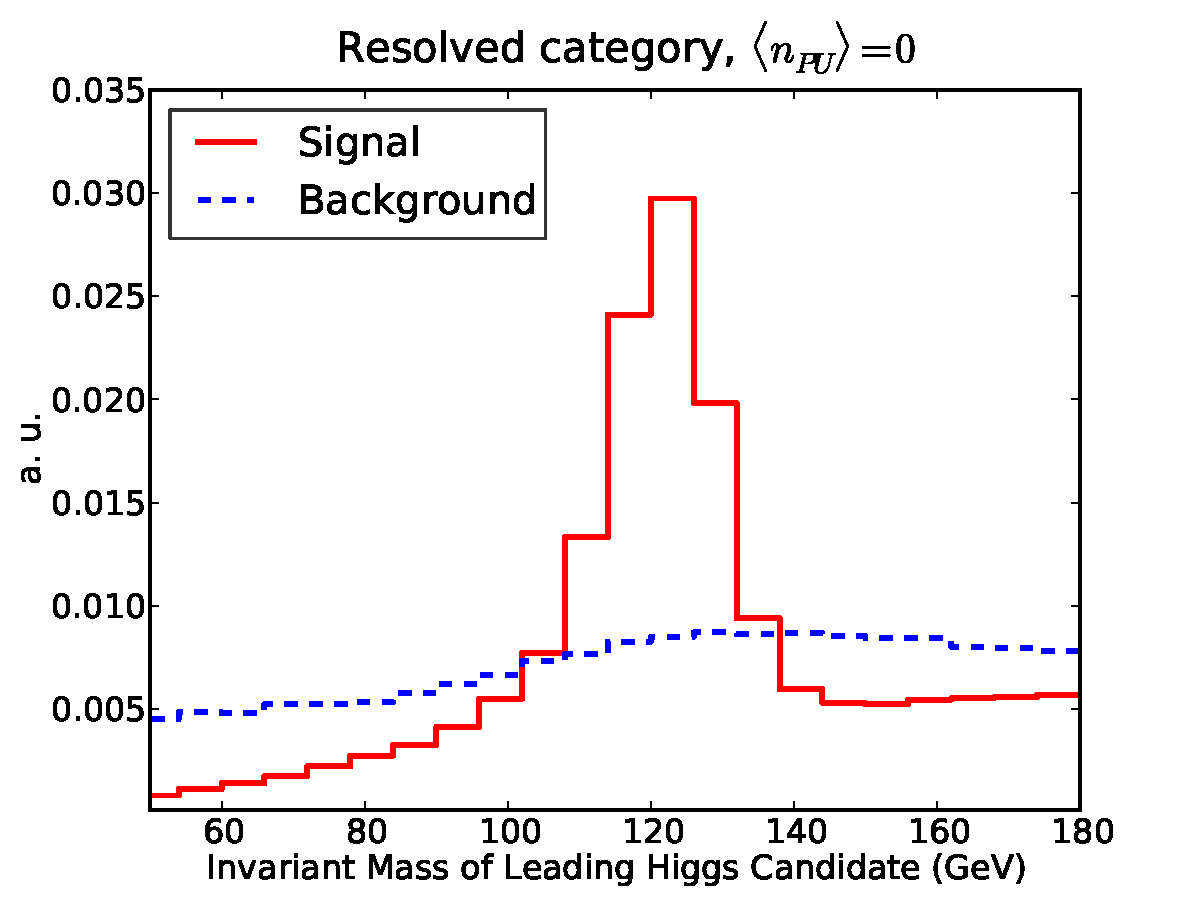
\includegraphics[width=0.48\textwidth]{plots/m_H0_res_C1d_noPU.pdf}
  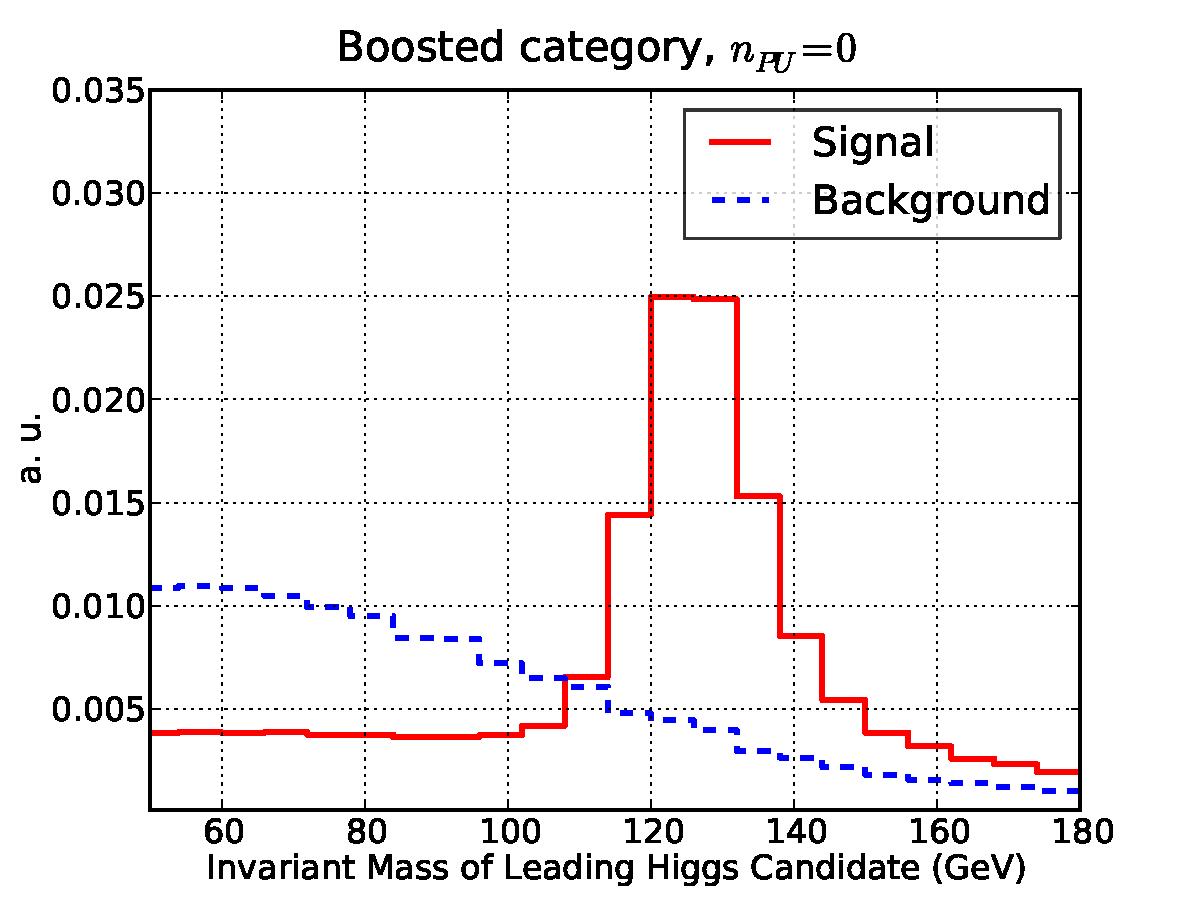
\includegraphics[width=0.48\textwidth]{plots/m_H0_bst_C1d_noPU.pdf}
  \caption{\small Same as   Fig.~\ref{fig:cutplots1} for the invariant
    mass distribution of the leading Higgs candidates in the resolved
    (left plot) and boosted (right plot) selections.
}
\label{fig:mHHinv}
\end{center}
\end{figure}
%%%%%%%%%%%%%%%%%%%%%%%


Another important kinematic distribution for
this process is the invariant mass
of the di-Higgs system.
%
This is a direct measure of the boost of the system,
which in  BSM scenarios can be substantially
enhanced, for instance due to
specific $d=6$ EFT operators~\cite{Azatov:2015oxa}.
%
One important advantage of the $b\bar{b}b\bar{b}$ final state for
di-Higgs production is that it significantly increases the reach
in $m_{hh}$ as compared to other channels with smaller branching
ratios,
such as $2b2\gamma$ or $2b2\tau$.
%
In Fig.~\ref{fig:mhh} we show the invariant mass distribution of the
reconstructed Higgs pairs,
comparing the resolved and the boosted categories.

%%%%%%%%%%%%%%%%%%%%%%%%%%%%%%%%%%%%%%%%%%%%%%%
\begin{figure}[t]
\begin{center}
  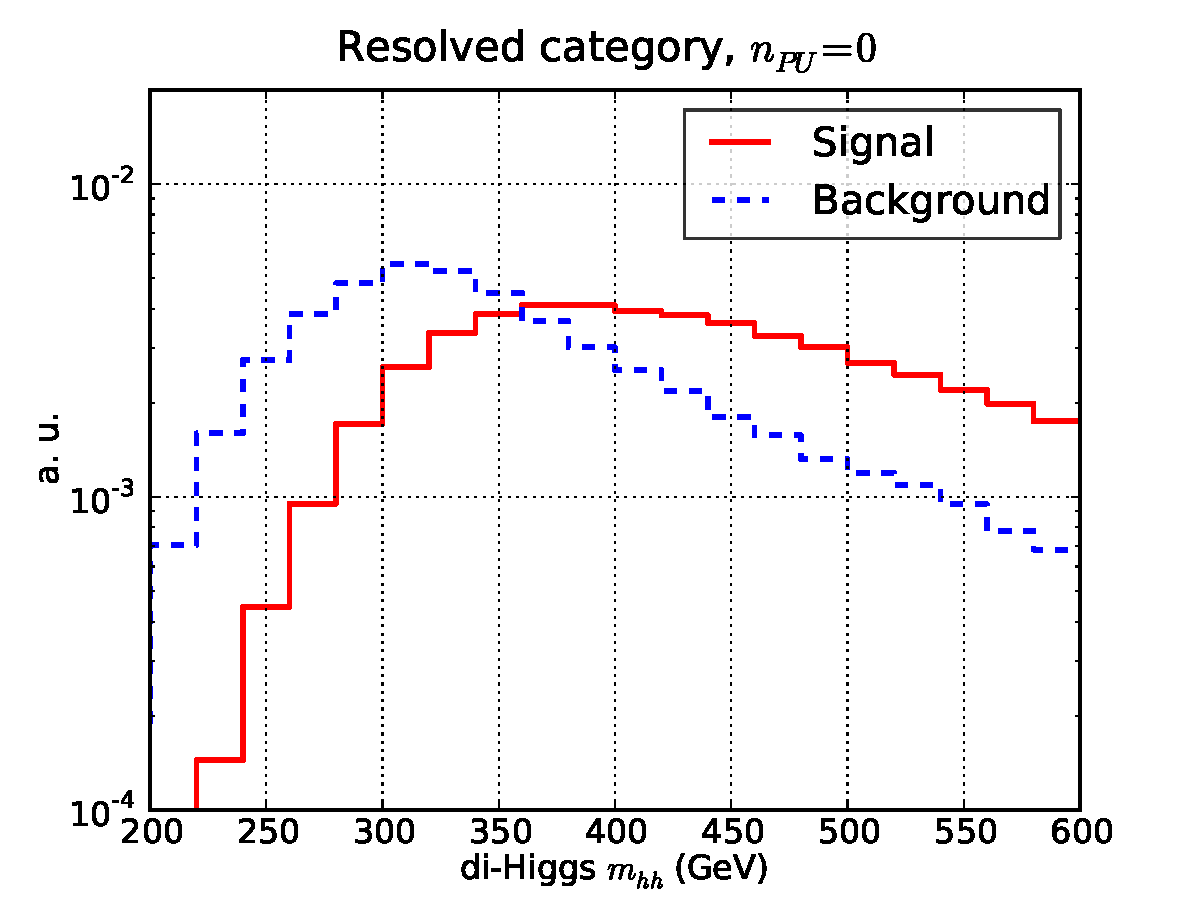
\includegraphics[width=0.48\textwidth]{plots/m_HH_C2_res_noPU.pdf}
  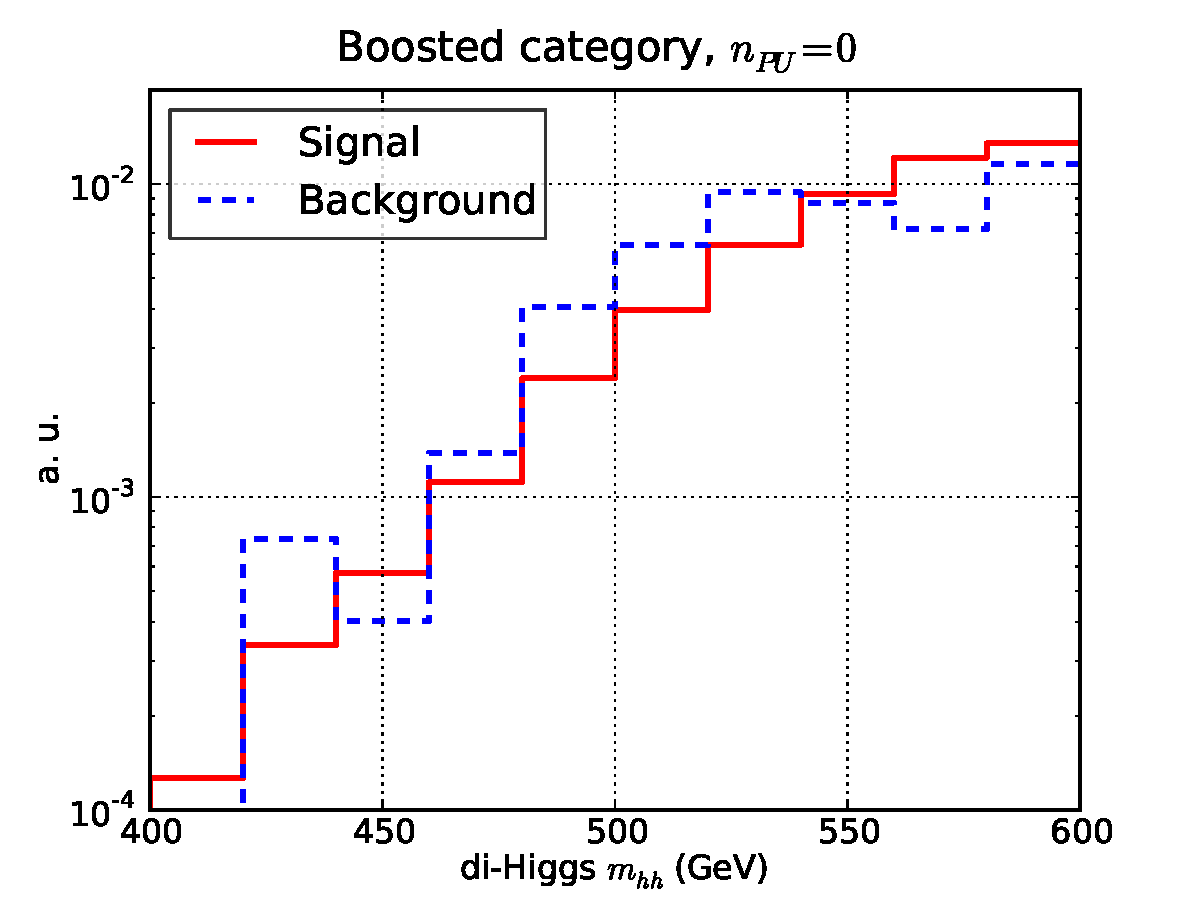
\includegraphics[width=0.48\textwidth]{plots/m_HH_C2_bst_noPU.pdf}
  \caption{\small
Same as   Fig.~\ref{fig:cutplots1} for the invariant
mass distribution of the di-Higgs system $m_{hh}$, in
the resolved (left plot) and boosted (right plot) categories.
}
\label{fig:mhh}
\end{center}
\end{figure}
%%%%%%%%%%%%%%%%%%%%%%%%%%%%%%%%%%%%%%%%%%%%%%%%%

In the resolved case, we see that the distribution
in $m_{hh}$ is rather harder for the signal as compared
to the background,
and thus one expects that cutting in $m_{hh}$ would help signal
discrimination: we will verify this using the MVA.
%
For the boosted category the overall trend of the $m_{hh}$ distribution
is different because of the jet selection criteria, and the
distribution now peaks at higher values of the invariant mass.
%
In this case, signal and background distributions
look similar.
%
Note that at parton-level the $m_{hh}$ distribution
for signal events has a kinematic
cut-off at $m_{hh}^{\rm min}=250$ GeV, which is smeared due
to 
the parton shower and to detector resolution effects.
%


In Fig.~\ref{fig:pthh} we show the transverse momentum of
the di-Higgs system, $p_T^{hh}$,
for the resolved and boosted categories.
%
Again we see that the background has a steeper $p_T^{hh}$ distribution
that the signal, in both categories, thus this variable
should provide additional discrimination power, and therefore
this distribution is one of the inputs for the MVA.
%
In our LO simulation the $p_T^{hh}$ distribution is generated
by the parton shower, and improved theoretical
description would require
either the matching with higher-multiplicity
matrix elements~\cite{Maierhofer:2013sha} or
the full NLO calculation~\cite{Frederix:2014hta},
%
Nevertheless, as we will show,
the MVA shows only limited sensitivity to this variable, so its
modelling is not crucial in this specific application.

%%%%%%%%%%%%%%%%%%%%%%%%%%%%
\begin{figure}[t]
\begin{center}
  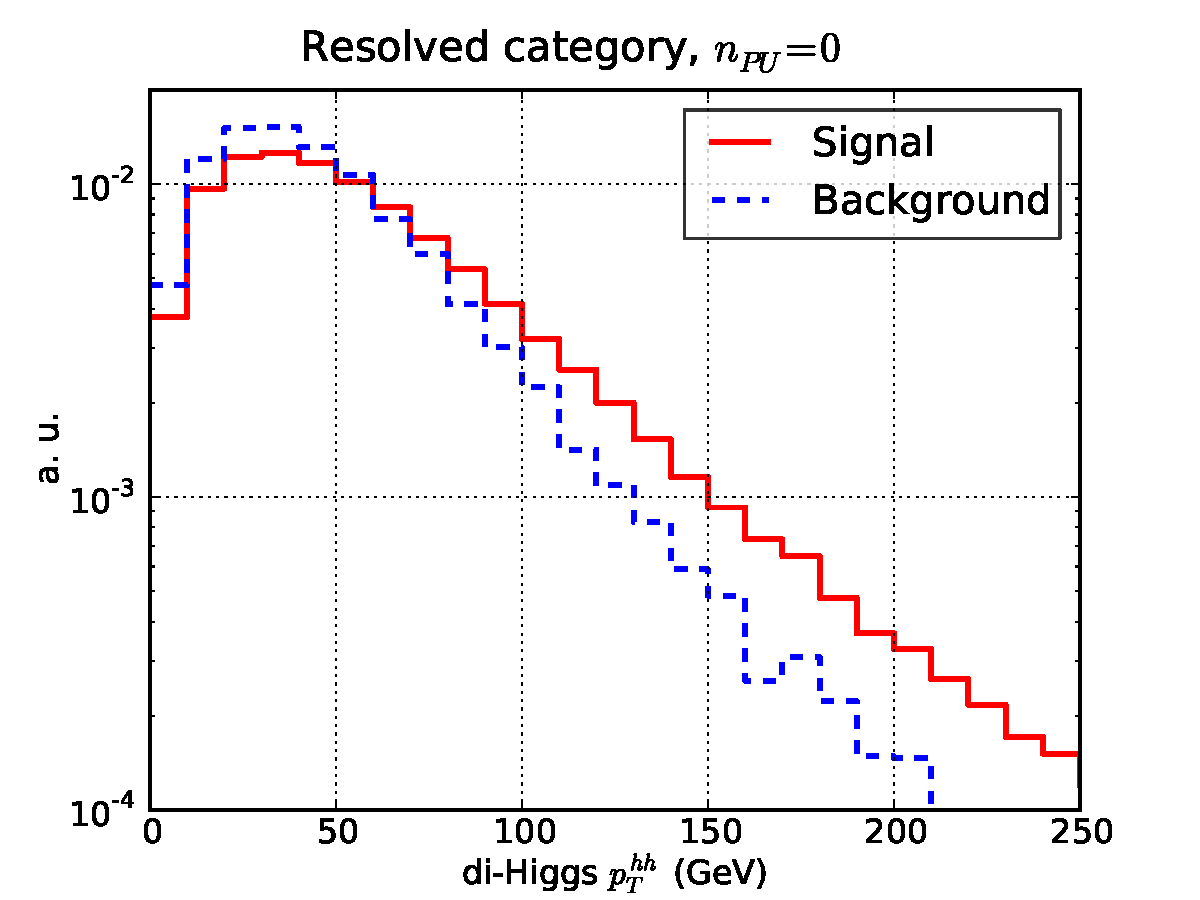
\includegraphics[width=0.48\textwidth]{plots/pt_HH_C2_res_noPU.pdf}
  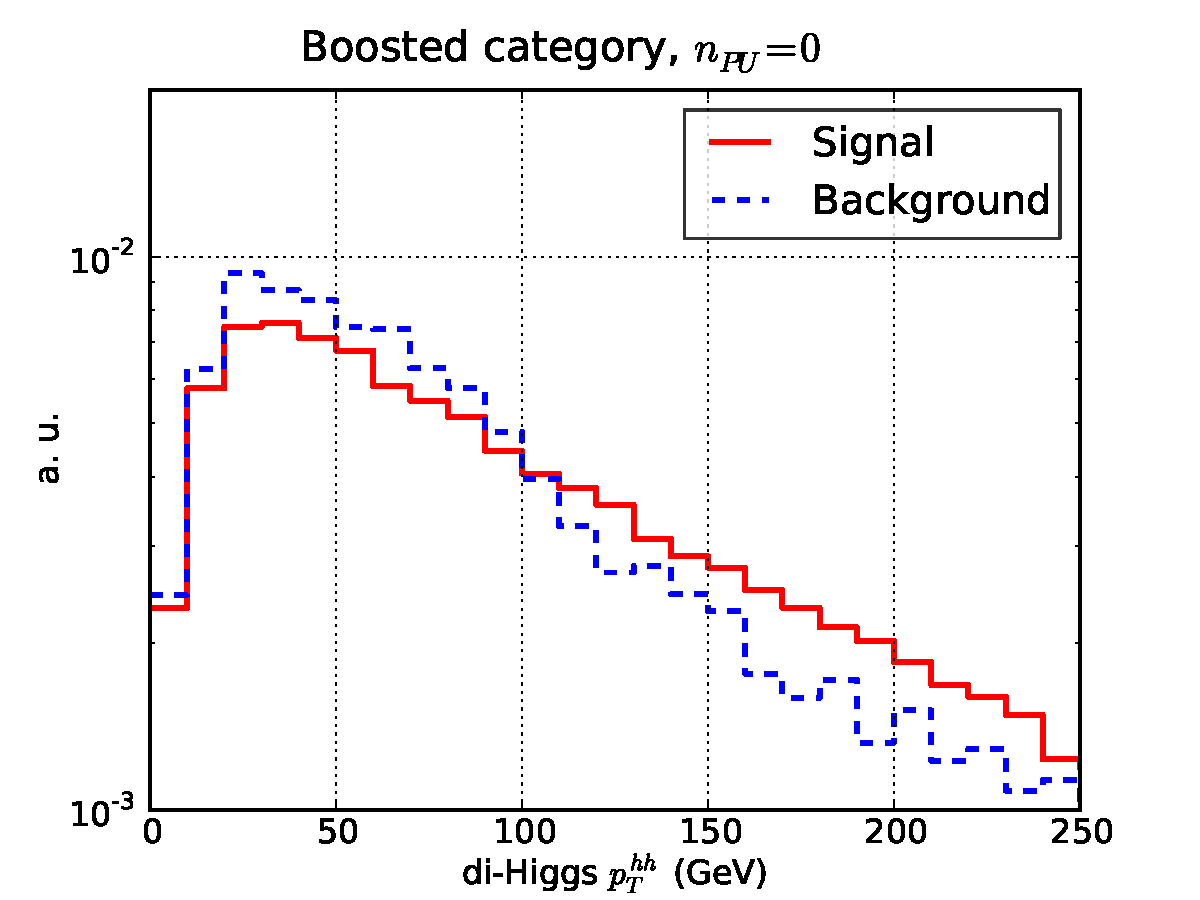
\includegraphics[width=0.48\textwidth]{plots/pt_HH_C2_bst_noPU.pdf}
  \caption{\small Same as Fig.~\ref{fig:mhh} for the transverse momentum
    distribution of the di-Higgs system $p_T^{hh}$.
}
\label{fig:pthh}
\end{center}
\end{figure}
%%%%%%%%%%%%%%%%%%%%%%%


We now study the discrimination power to separate signal
and background events contained in
jet substructure
variables.
%
In Fig.~\ref{fig:mva_substructure_1}
we show the distributions of representative
 substructure variables for the boosted category: the
$k_t$ splitting scale $\sqrt{d_{12}}$, Eq.~(\ref{eq:ktsplitting}), 
the ECF ratio $C_2^{(\beta)}$,
Eq.~(\ref{eq:c2}), and
the 2--to--1 subjettiness ratio $\tau_{12}$, Eq.~(\ref{eq:tau21}),
all for the leading
Higgs candidates, and also $\tau_{12}$ for the subleading
Higgs candidates.

%%%%%%%%%%%%%%%%%%%%%%%%%%%%%%%%%%%%%%%%%%%%%%%%%%%%%%%
\begin{figure}[t]
  \begin{center}
    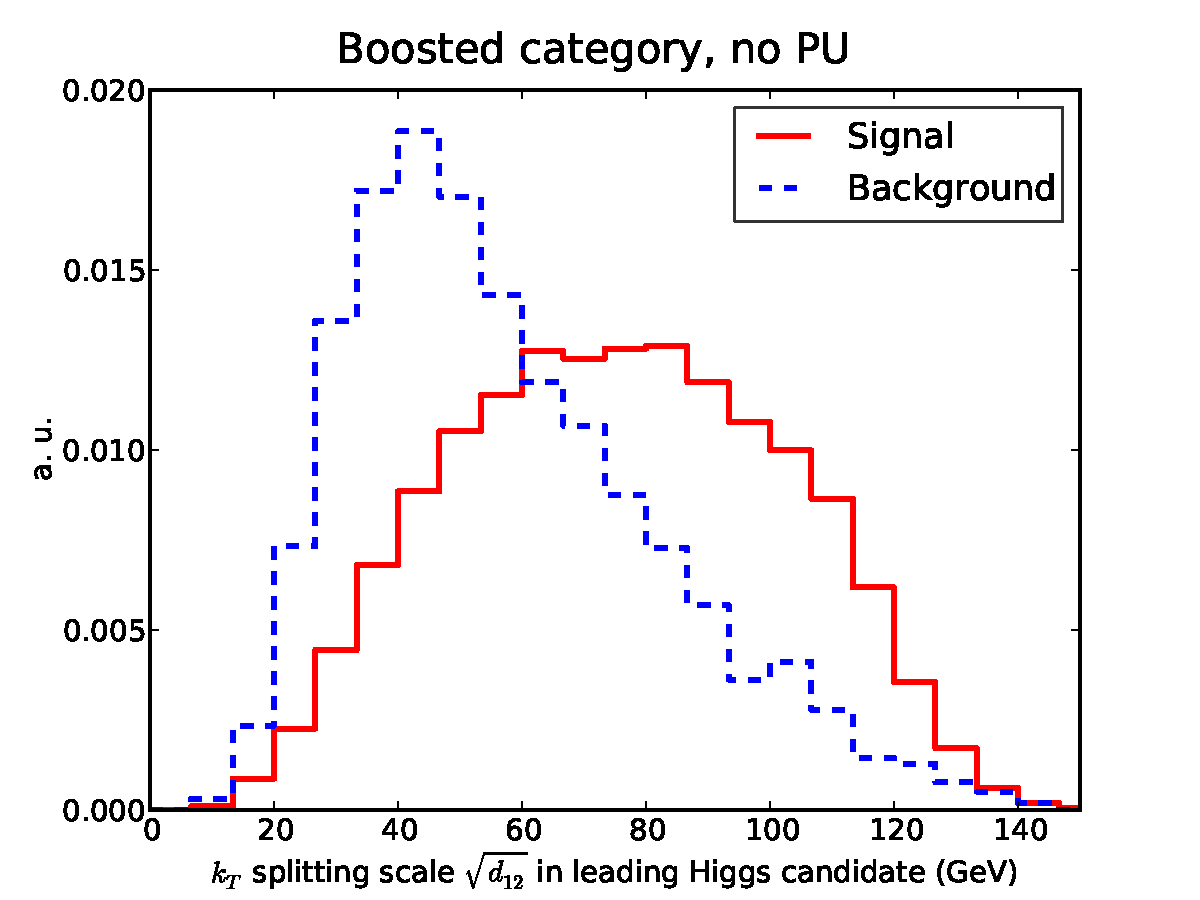
\includegraphics[width=0.48\textwidth]{plots/split12_h1_C1_boost.pdf} 
  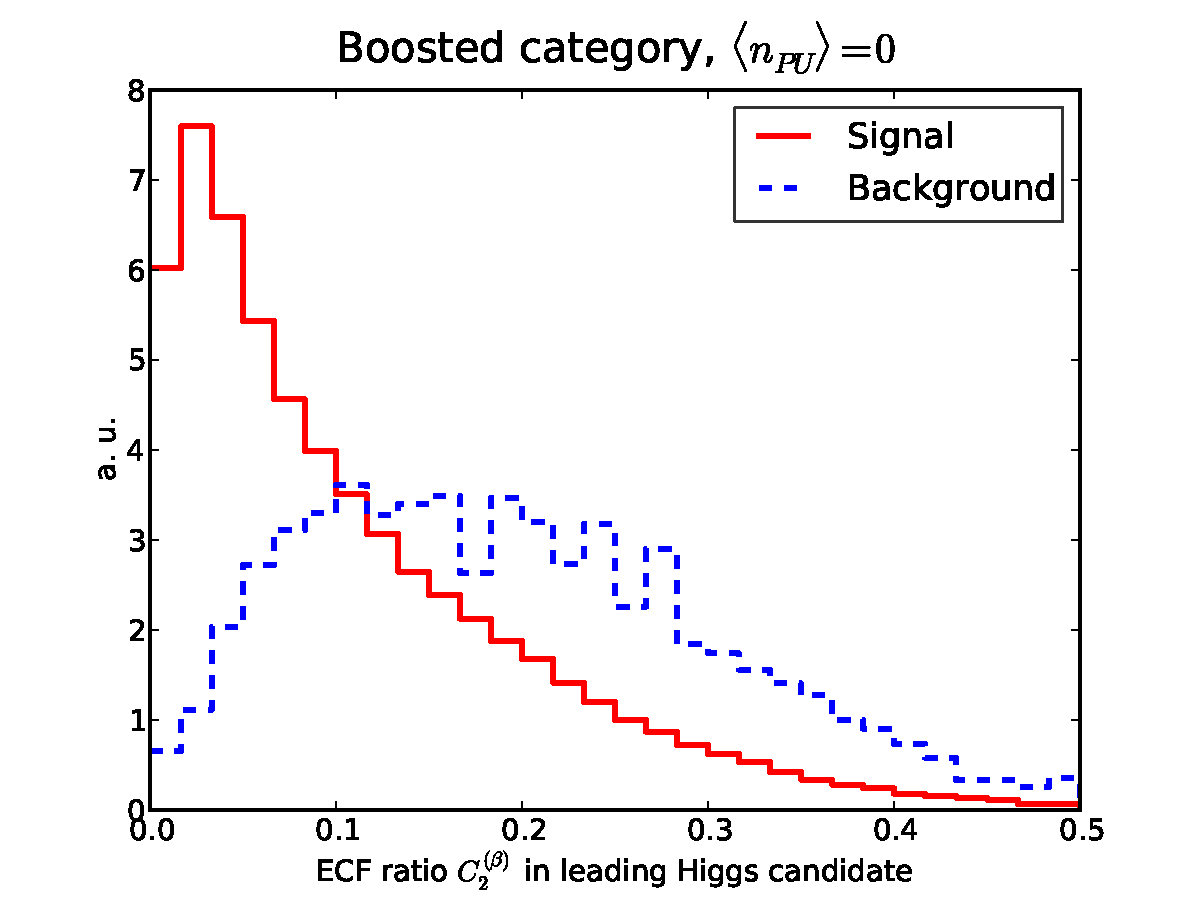
\includegraphics[width=0.48\textwidth]{plots/EEC_C2_h0_C1_boost.pdf}
  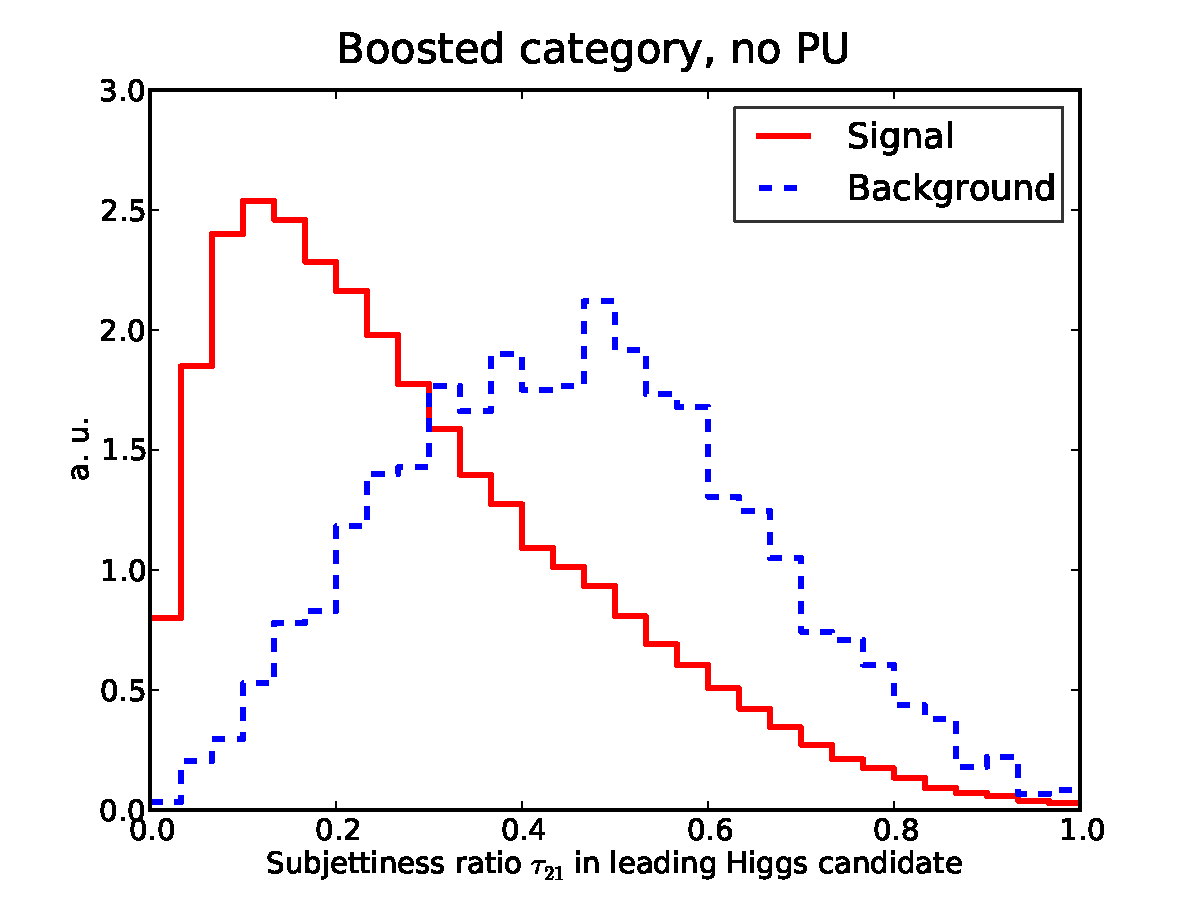
\includegraphics[width=0.48\textwidth]{plots/tau21_h0_C1_boost.pdf}
  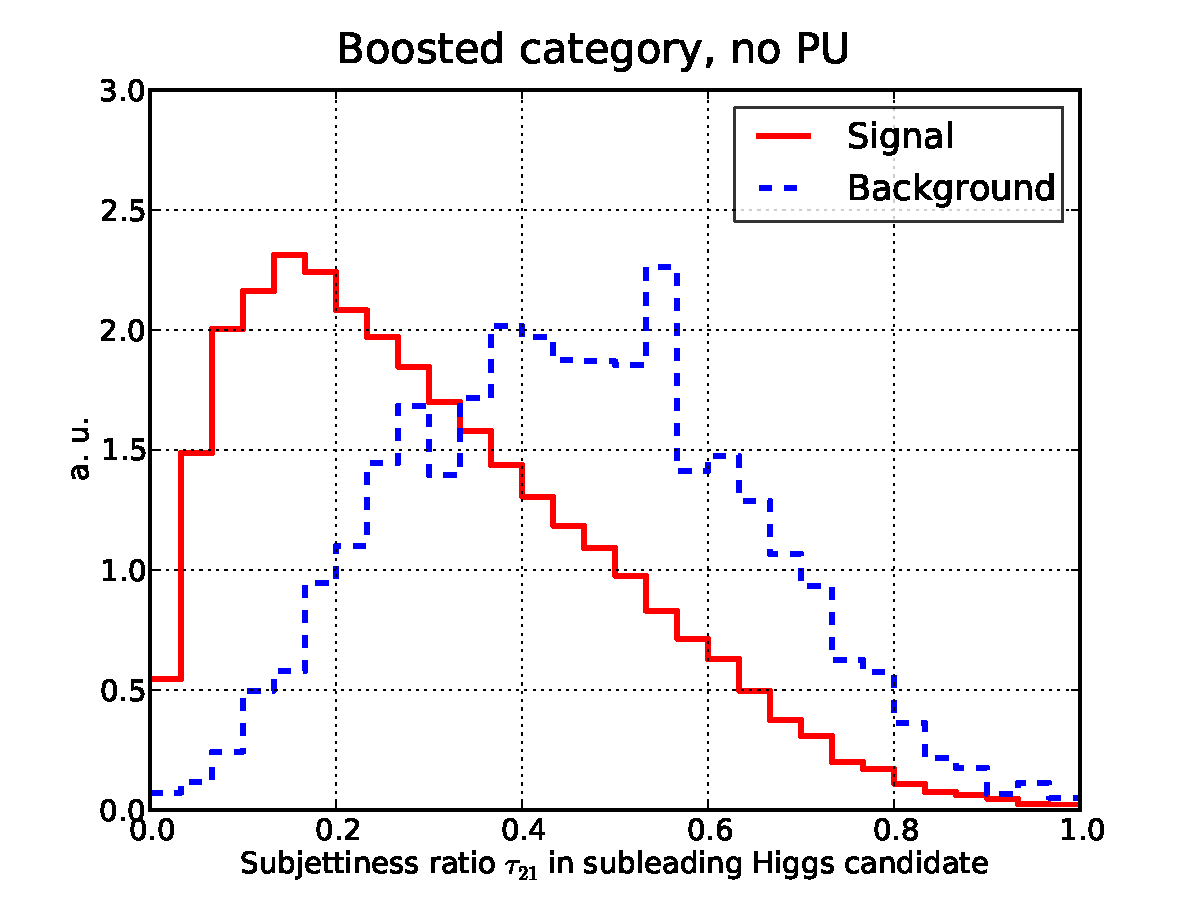
\includegraphics[width=0.48\textwidth]{plots/tau21_h1_C1_boost.pdf}
  \caption{\small Distribution of representative substructure variables
    in the boosted category at the end of the cut-based
    analysis, to be used as input to the MVA.
    %
    From top to bottom and from left to right we show  the
    $k_t$ splitting scale, the energy correlation ratio $C_2^{(\beta)}$
    and the  subjettiness ratio $\tau_{21}$ for the leading
    Higgs, as well as $\tau_{21}$ also for the subleading Higgs.
}
\label{fig:mva_substructure_1}
\end{center}
\end{figure}
%%%%%%%%%%%%%%%%%%%%%%%%%%%%%%%%%%%%%%%%%%%%%%%%%%%%%%%%%%%%%%%%%%%


From Fig.~\ref{fig:mva_substructure_1}
we can observe how for these substructure variables the shapes of the signal
and background distributions reflect
the inherent differences in the internal structure of jets
between QCD jets and jets originated from the Higgs decays.
%
Signal and background distributions peak
in rather
different regions: for example, the $k_t$ splitting scale $\sqrt{d_{12}}$
peaks around 80 GeV (40 GeV) for signal (background) events, while
the distribution of the
ECF ratio $C_2^{(\beta)}$ is concentrated at small values
for signal but is much broader for background events.
%
From Fig.~\ref{fig:mva_substructure_1} we also see
the distributions of the subjettiness ratio $\tau_{12}$ are
reasonably similar
for both the leading and the subleading jets.
%
Therefore, while we do not explicitly have cuts in the substructure
variables, their discrimination power between signal and
background events is the motivation to include them
as input to the MVA, as discussed in Sect.~\ref{sec:mva}.


\subsection{Impact of pile-up}
\label{sec:pileup}

Now we turn to discuss how the description of kinematic
distributions for $hh\to 4b$ signal
and background processes are
modified in a high pile-up (PU) environment.
%
To study the impact of PU,
Minimum Bias (MB) events,
including Multiple Parton Interactions (MPI), have been generated
with {\tt Pythia8}, and then
superimposed to the signal
and background samples described in Sect.~\ref{mcgeneration}.
%
We have explored two scenarios,
one with a mean number of
PU vertices per bunch crossing of $\la n_{\rm PU}\ra=80$, and another
with $\la n_{\rm PU}\ra=150$.
%
While the latter is closer to the HL-LHC forecasts,
we adopt $\la n_{\rm PU}\ra=80$ as our baseline,
given that it
is beyond the scope of this paper to fully optimize
the PU subtraction.

%
In order to subtract PU in hadronic collisions, a number of techniques
are available~\cite{Cacciari:2009dp,TheATLAScollaboration:2013pia,Butterworth:2008iy,Cacciari:2007fd,Krohn:2009th,Krohn:2013lba,Ellis:2009me,Bertolini:2014bba,Cacciari:2014gra,Cacciari:2014jta,Berta:2014eza,Larkoski:2014wba}.\footnote{
These techniques have also important applications in the subtraction
of the UE/MPI contamination for jet reconstruction
in heavy ion collisions~\cite{Cacciari:2010te}.
}
%
In this work, PU  will be subtracted by means
of the {\tt SoftKiller} (SK)
method~\cite{Cacciari:2014gra}, as implemented in {\tt FastJet},
whose performance has been shown to
improve the commonly used area-based subtraction~\cite{Cacciari:2009dp}.
%
The idea underlying {\tt SoftKiller} is based on eliminating particles
below a given cut-off in their transverse momentum, $p_T^{\rm (cut)}$, whose
value is dynamically determined in a way that makes the event-wide
transverse-momentum flow density $\rho$ vanish.
%
This $p_T$ flow density is defined as
\be
\rho\equiv{\rm median}_i \Bigg\{ \frac{p_{Ti}}{A_i}\Bigg\} \, ,
\ee
where the median is computed over all the patches $i$ with area
$A_i$ and transverse momentum $p_{Ti}$ in which the $\lp \eta,\phi\rp$ plane
is partitioned.
%
From its definition in terms of the median,
it follows that the value of $p_T^{(\rm cut)}$
will be dynamically raised until half of the patches have
$p_{Ti}=0$.
%
The size and number of these patches is a free parameter of the algorithm -
here we will use square patches with length $a=0.4$.
%
We restrict ourselves to the central rapidity region,
$|\eta| \le 2.5$, for the estimation of the
$p_T$ flow density $\rho$.
%
We apply {\tt SoftKiller}
to particles at the end of the parton shower, before
jet clustering.


%%%%%%%%%%%%%%%%%%%%%%%%
\begin{figure}[t]
  \begin{center}
  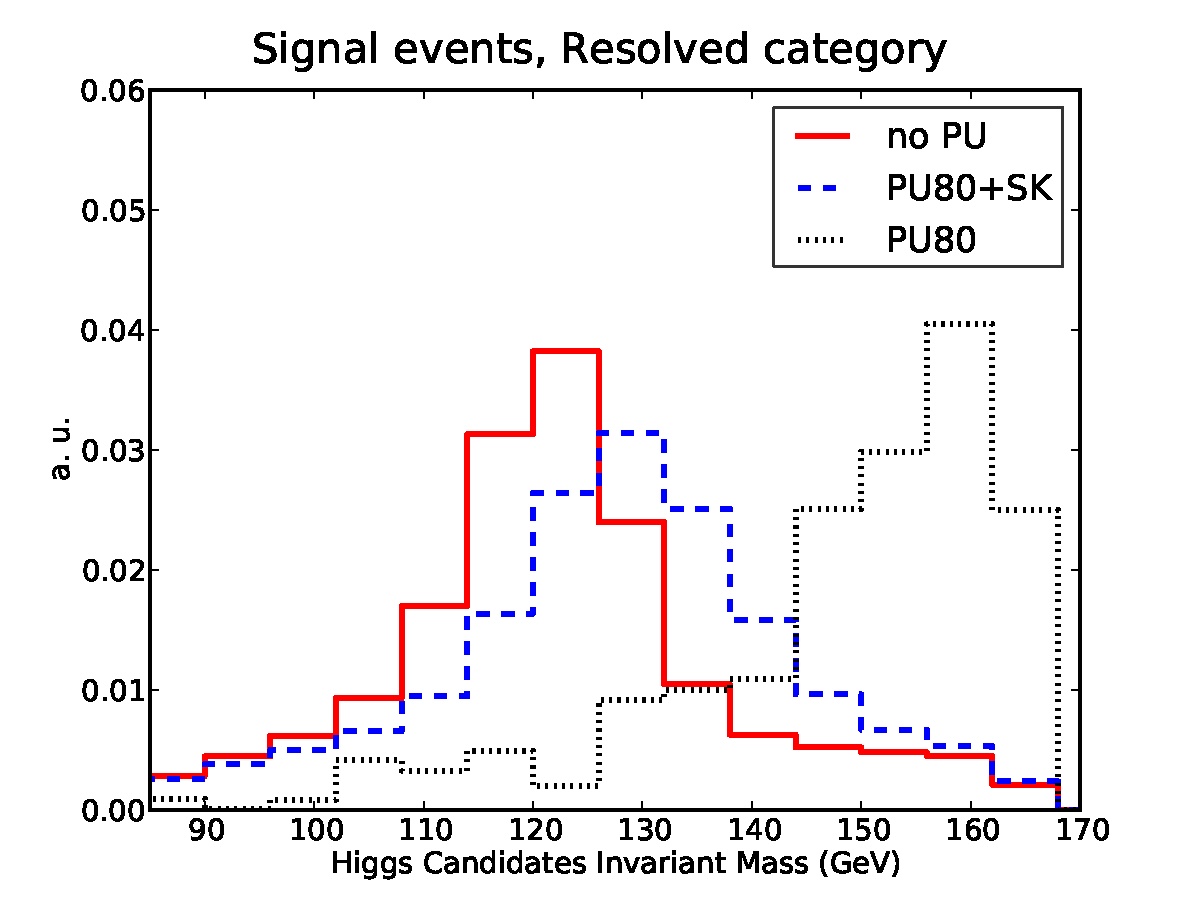
\includegraphics[width=0.63\textwidth]{plots/m_htot_res_signal_PUnoSK.pdf}
    \caption{\small
    The invariant mass distributions of Higgs candidates in signal
events, in the resolved category, comparing the results without PU,
with PU $\la n_{\rm PU}\ra=80$ but without any subtraction, and the
corresponding results now with SK subtraction.
}
\label{fig:PUvalidation}
\end{center}
\end{figure}
%%%%%%%%%%%%%%%%%%%%%%%

To validate PU subtraction,
we now compare representative kinematic distributions
in the case without PU and in the case
with PU subtracted with {\tt SoftKiller}.
%
We compare first
in Fig.~\ref{fig:PUvalidation} the
invariant mass distributions of Higgs candidates for signal
events in the resolved category.
%
We show three curves: without PU,
with PU $\la n_{\rm PU}\ra=80$ but without any subtraction, and the
same but now with the SK subtraction.
%
If PU is not subtracted there is a large shift in the Higgs mass
peak, by about 40 GeV.
%
Once SK subtraction is performed, we recover a distribution much closer
to the original ones, with only a small shift of $\simeq 5$ GeV
and a broadening of the mass
distribution.
%


Next, we compare additional
 distributions with
and without PU, with $\la n_{\rm PU}\ra=80$ in the
former
case (and SK subtraction).
%
In Fig.~\ref{fig:m_H_PU} we show the invariant mass distribution
of the leading and subleading Higgs candidates,
this time corresponding
to the boosted category.
%
These distributions are plotted after the $b$-tagging, that is,
before they are used as input to the MVA.
%
As we can see, the residual effects of PU
after the {\tt SoftKiller} subtraction are smaller
in the boosted selection as compared to the resolved case,
with the position of the Higgs mass peaks essentially
unchanged, and only a moderate broadening of the
mass distribution.
%

%%%%%%%%%%%%%%%%%%%%%%%%
\begin{figure}[t]
  \begin{center}
      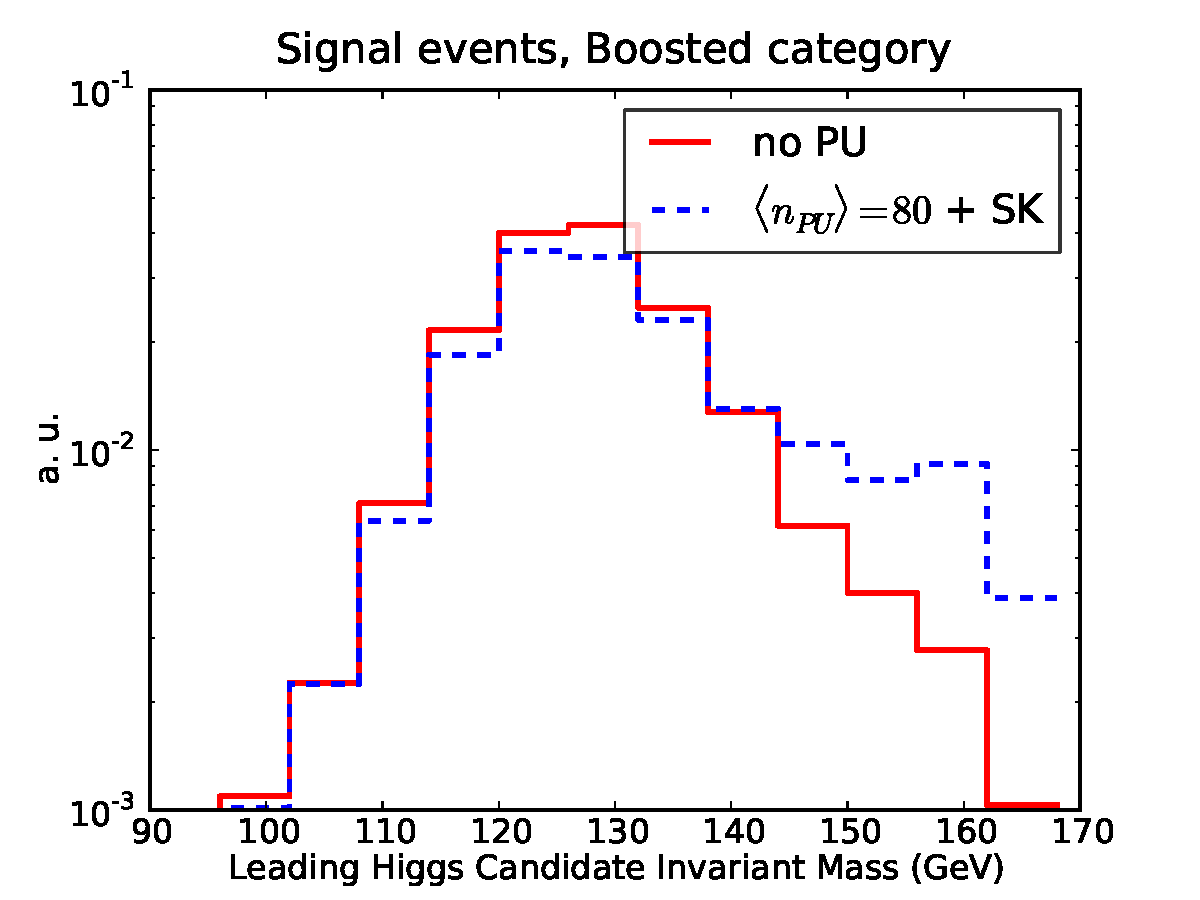
\includegraphics[width=0.49\textwidth]{plots/m_H0_bst_comp.pdf}
      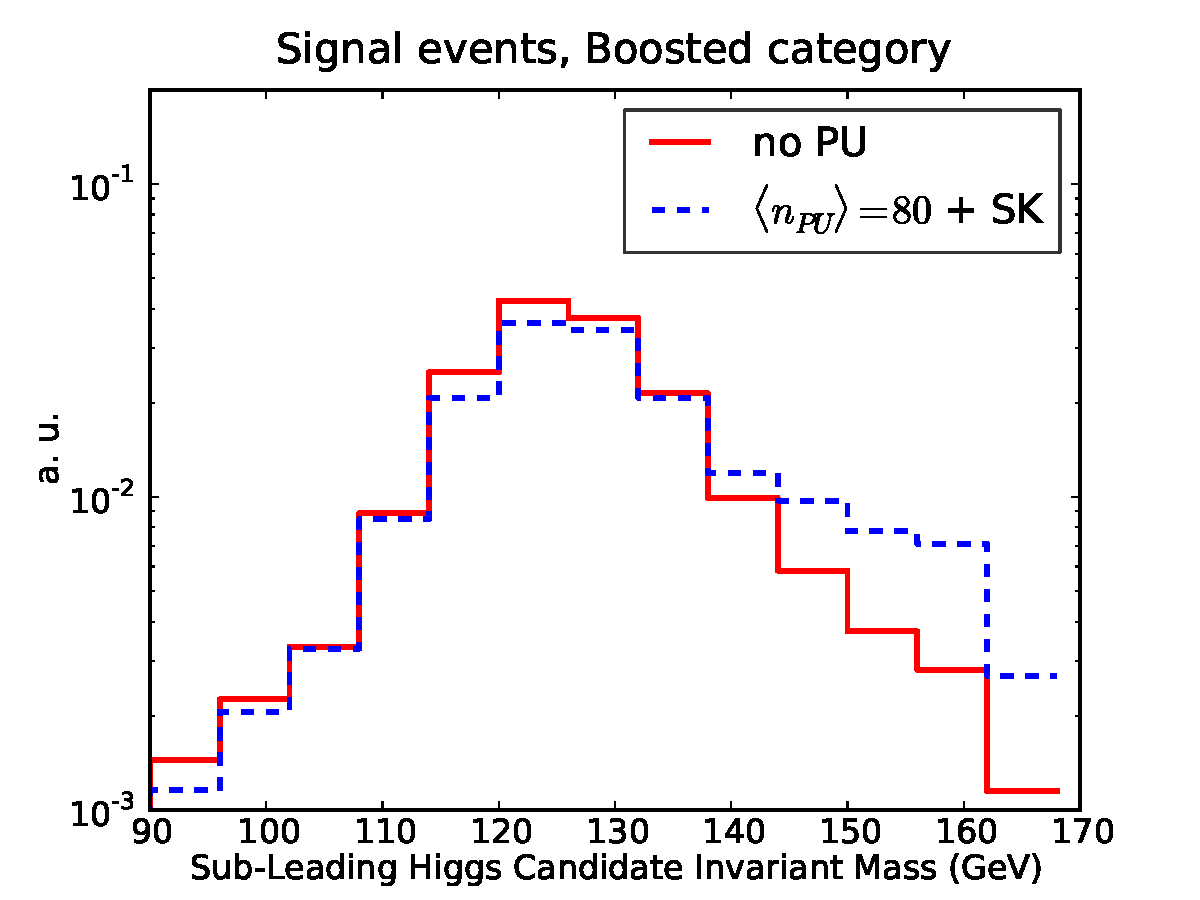
\includegraphics[width=0.49\textwidth]{plots/m_H1_bst_comp.pdf}
  \caption{\small
    Comparison of the invariant mass distributions of the leading (left plot)
    and subleading (right plot) Higgs candidates
    in the boosted category,
    both without PU and with
    PU, $\la n_{PU}\ra=80$, subtracted with {\tt SoftKiller}.
}
\label{fig:m_H_PU}
\end{center}
\end{figure}
%%%%%%%%%%%%%%%%%%%%%%%

In Fig.~\ref{fig:mHH_PU}
we compare the transverse momentum of the leading Higgs
candidate, $p_t^{h_1}$ and the invariant mass of the di-Higgs system
$m_{hh}$, in both for the boosted and
for the resolved categories.
%
In the case of the $p_T^{h1}$ distribution, the differences between the selection
criteria for the resolved
and boosted categories is reflected in the rightward shift of the latter.
%
The effect of PU is small in the boosted case, and generally moderate
in the resolved case, except for large $p_T$ values.
%
Similar observation can be derived for the case of
the di-Higgs invariant mass $m_{hh}$ distribution, similar 
apply.
%
Therefore, we can consider the PU subtraction strategy
as validated for the purposes of this study, although
there could still be room for optimisation.


%%%%%%%%%%%%%%%%%%%%%%%%
\begin{figure}[t]
  \begin{center}
  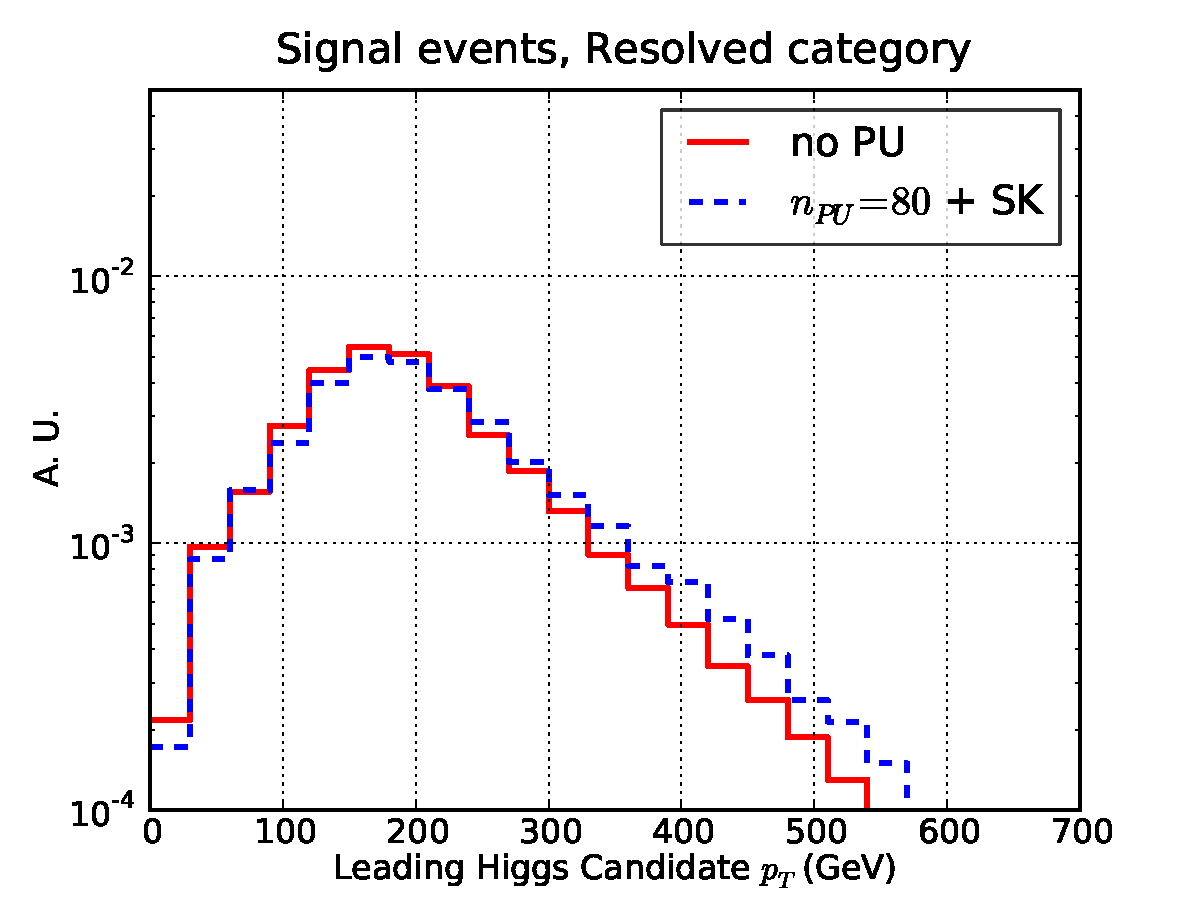
\includegraphics[width=0.49\textwidth]{plots/pt_H0_C2_res_comp.pdf}
  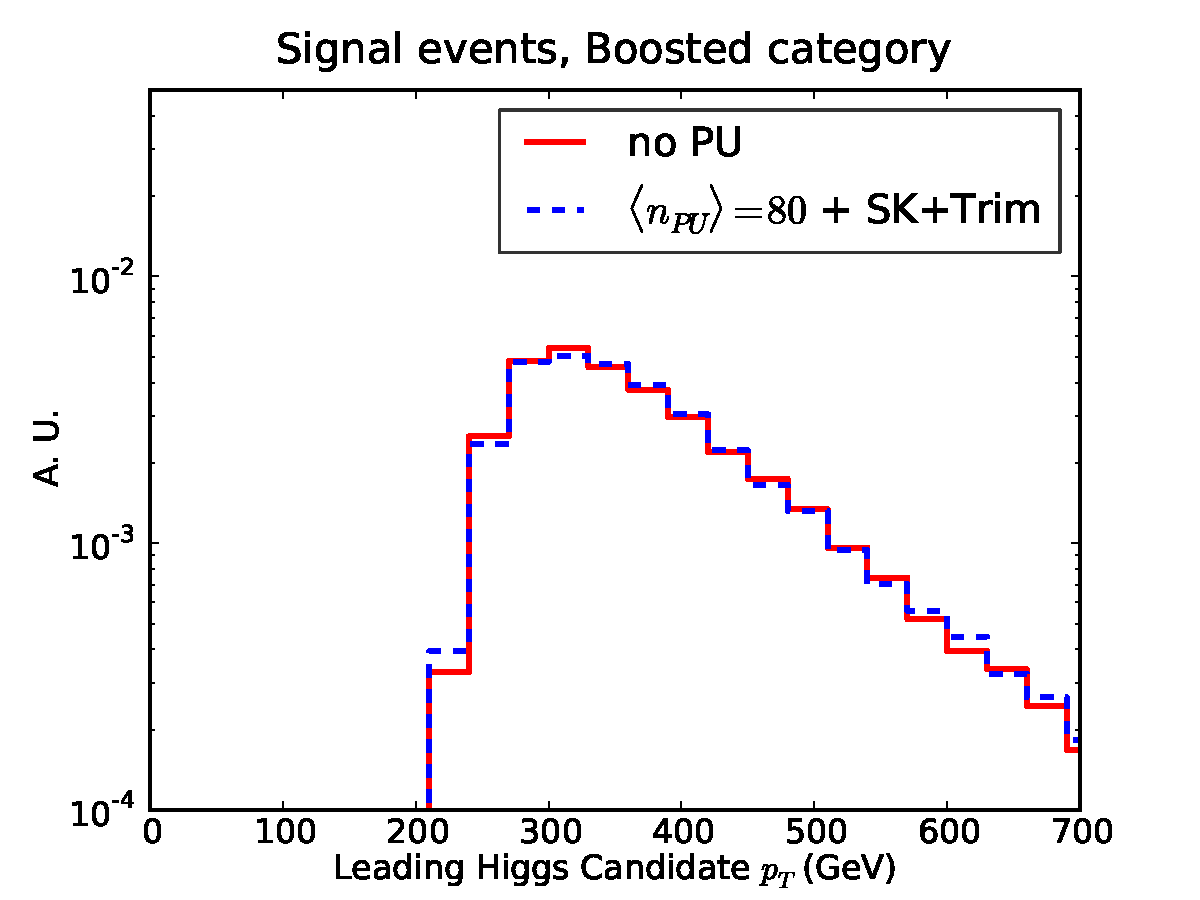
\includegraphics[width=0.49\textwidth]{plots/pt_H0_C2_bst_comp.pdf}
  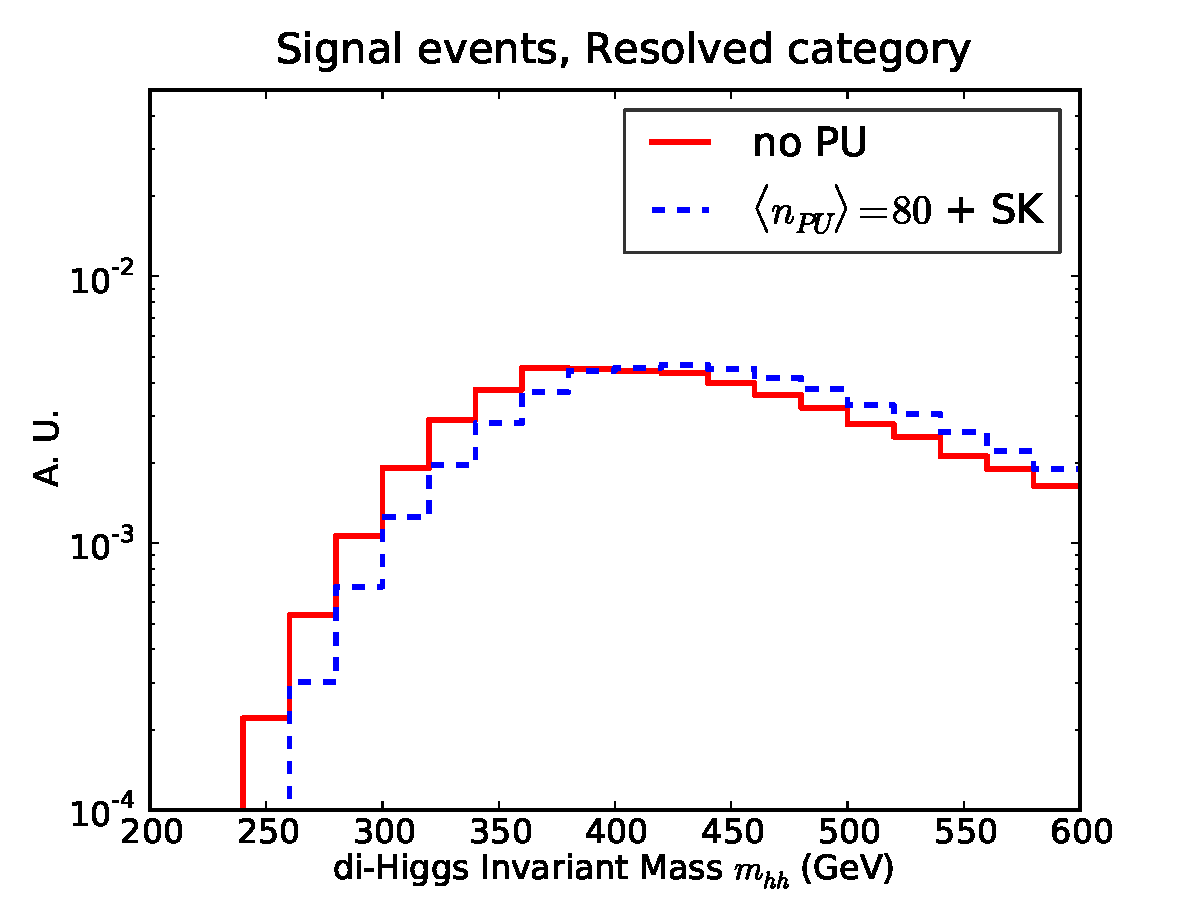
\includegraphics[width=0.49\textwidth]{plots/m_HH_C2_res_comp.pdf}
  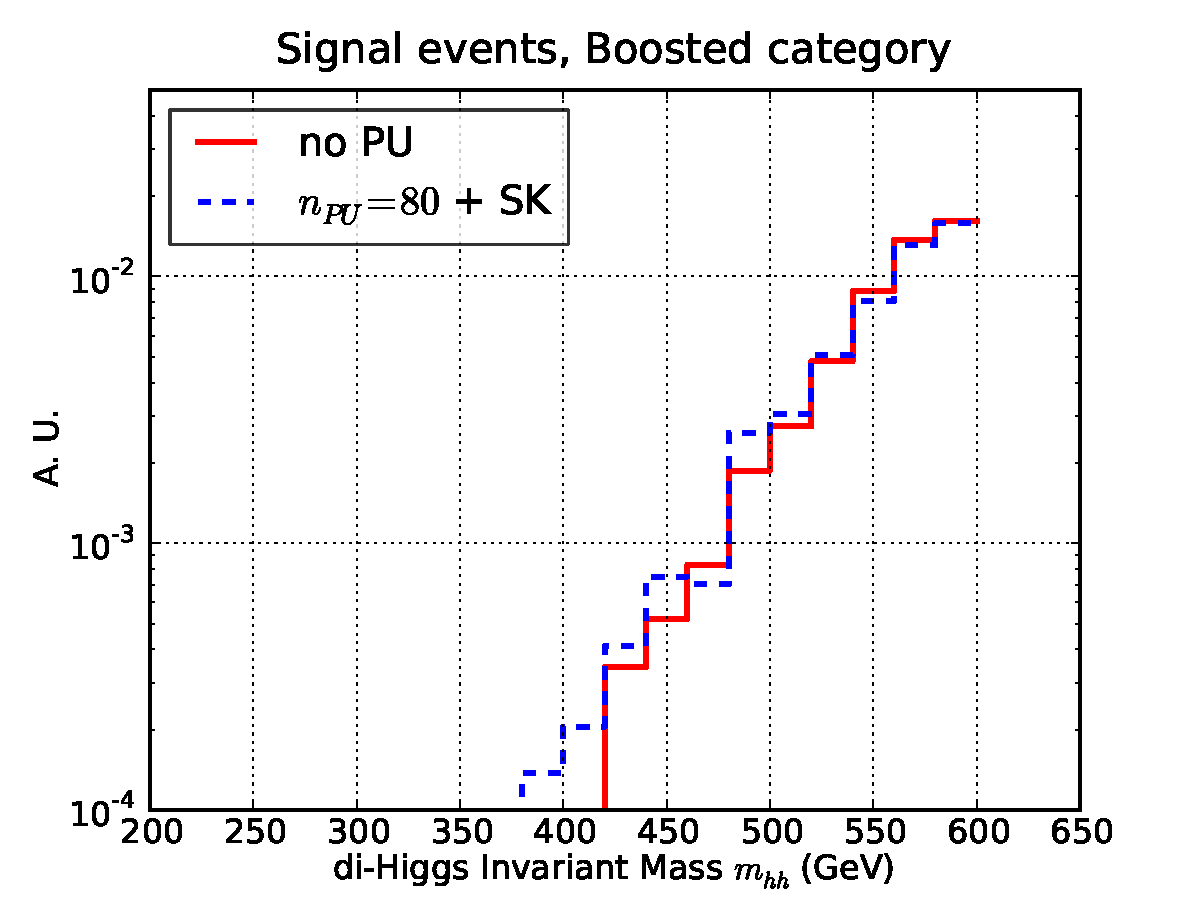
\includegraphics[width=0.49\textwidth]{plots/m_HH_C2_bst_comp.pdf}
  \caption{\small
    Comparison of the transverse momentum $p_T^h$ of the leading
    Higgs candidate (upper plots) and of the invariant mass $m_{hh}$
    of the di-Higgs system (lower plots) in the resolved
    (left plots) and boosted (right plots) categories,
    without PU and with $\la n_{PU}\ra=80$ subtracted with {\tt SoftKiller}.
}
\label{fig:mHH_PU}
\end{center}
\end{figure}
%%%%%%%%%%%%%%%%%%%%%%%

We can also assess the impact of PU in some of
substructure variables that will be 
used as input to the MVA in the boosted category.
%
In Fig.~\ref{fig:Substructure_PU} we show the 2-to-1 subjettiness ratio
$\tau_{21}$, Eq.~(\ref{eq:tau21}), and the ratio
of energy correlation functions, $D_2^{(\beta)}$,
Eq.~(\ref{eq:d2}), in both cases
corresponding to the leading Higgs candidate.
%
Comparing the signal distributions in the cases without PU and
with PU subtracted with SK, we observe that both substructure variables
are reasonably robust in a high-PU environment.
%
The ratio of energy correlation functions $D_2^{(\beta)}$ 
was indeed constructed~\cite{Larkoski:2013eya}
to be resilient
with respect to PU contamination.
%

%%%%%%%%%%%%%%%%%%%%%%%%
\begin{figure}[t]
  \begin{center}
  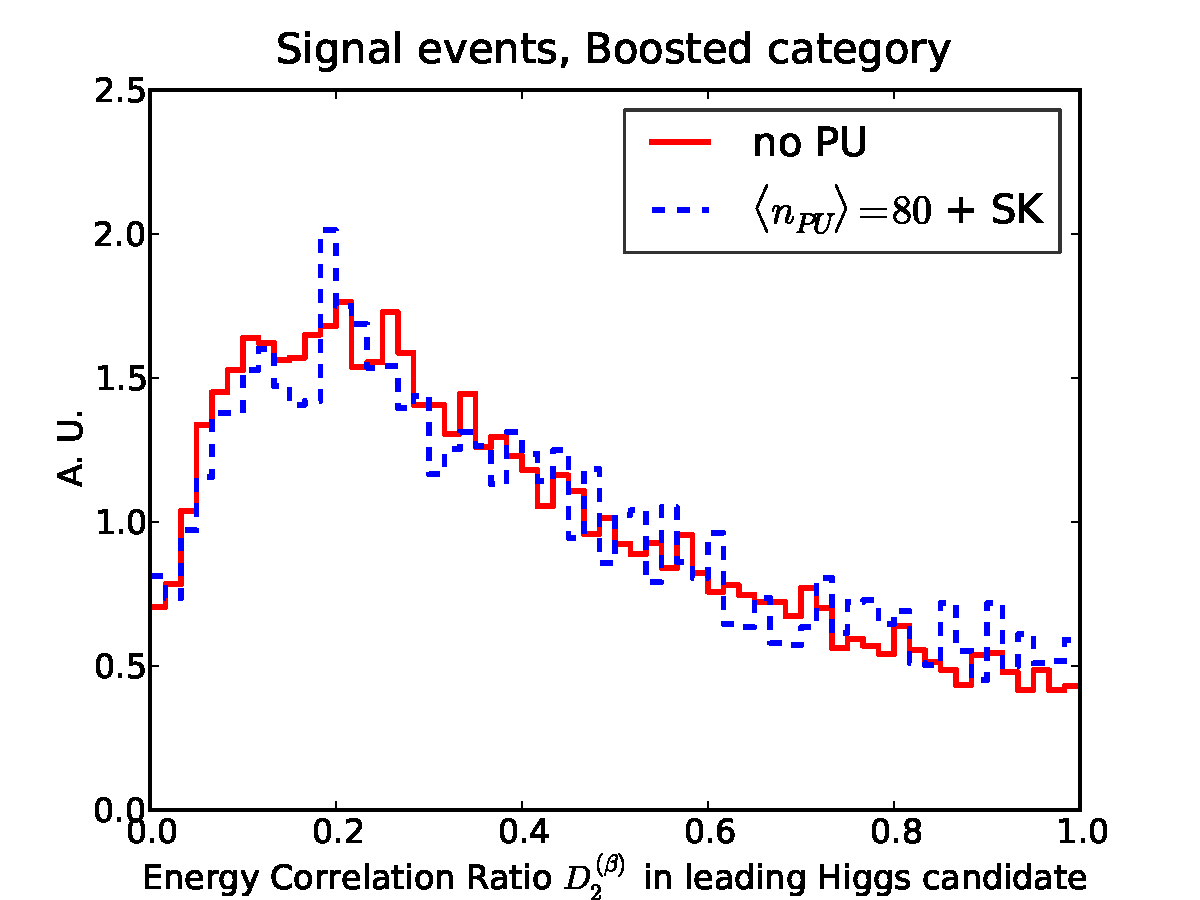
\includegraphics[width=0.49\textwidth]{plots/D2_h0_bst_comp.pdf}
  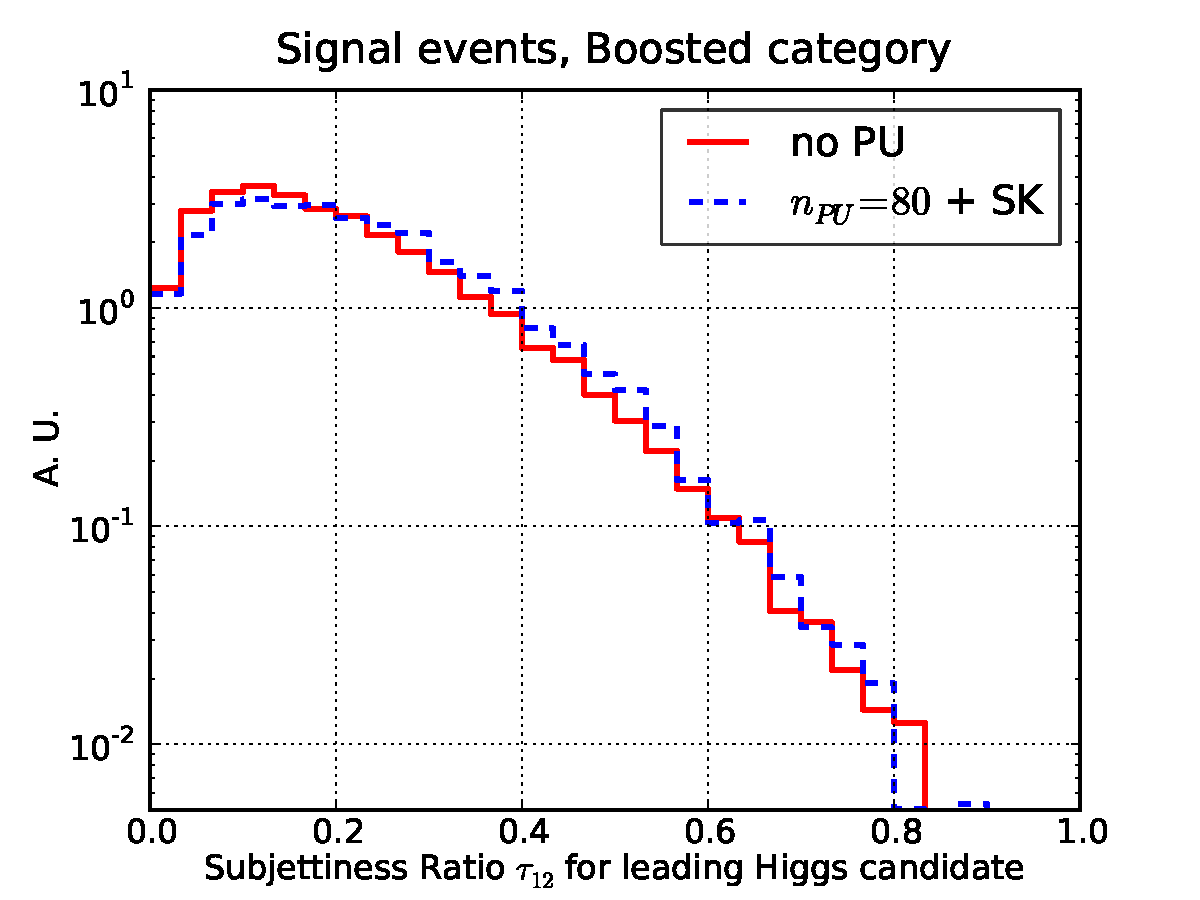
\includegraphics[width=0.49\textwidth]{plots/tau21_h0_bst_comp.pdf}
   \caption{\small
     Comparison of the substructure variables $D_2^{(\beta)}$ (left)
     and $\tau_{21}$ (right)
     for the leading Higgs candidate in the boosted category,
   without PU and with $\la n_{\rm PU}\ra=80$ subtracted with {\tt SoftKiller}.
}
\label{fig:Substructure_PU}
\end{center}
\end{figure}
%%%%%%%%%%%%%%%%%%%%%%%

It is also interesting to quantify how
the relative differences between
signal over background distributions are modified in a high-PU
environment.
%
Considering first of all the boosted category,
in Fig.~\ref{fig:signal-vs-back-boosted} we compare
various kinematic distributions for signal and background events,
with and without PU for the leading Higgs candidate: the invariant mass, the transverse
momentum distribution $p_T$,
     the 2--to--1 subjettiness ratio $\tau_{21}$, and 
     the $k_T$ splitting scale $\sqrt{d_{12}}$, Eq.~(\ref{eq:ktsplitting}).
     %
      We verify that the relevant
      qualitative differences between signal
      and background distributions are maintained even in the presence of PU.
      %
      This is specially noticeable for the substructure variables, which
      exhibit a similar discrimination power both with and without
      PU.
     

%%%%%%%%%%%%%%%%%%%%%%%%
\begin{figure}[t]
  \begin{center}
  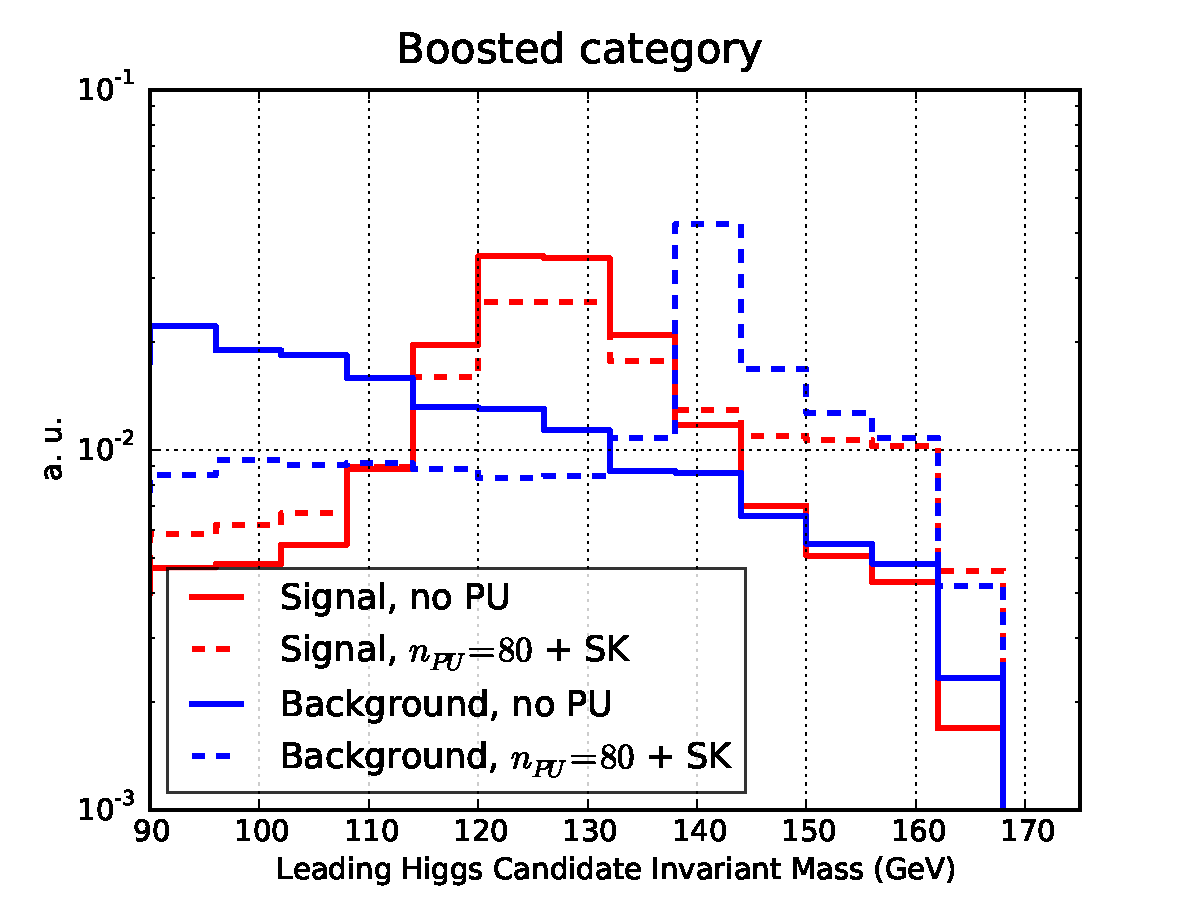
\includegraphics[width=0.49\textwidth]{plots/m_h0_bst_comp_back.pdf}
  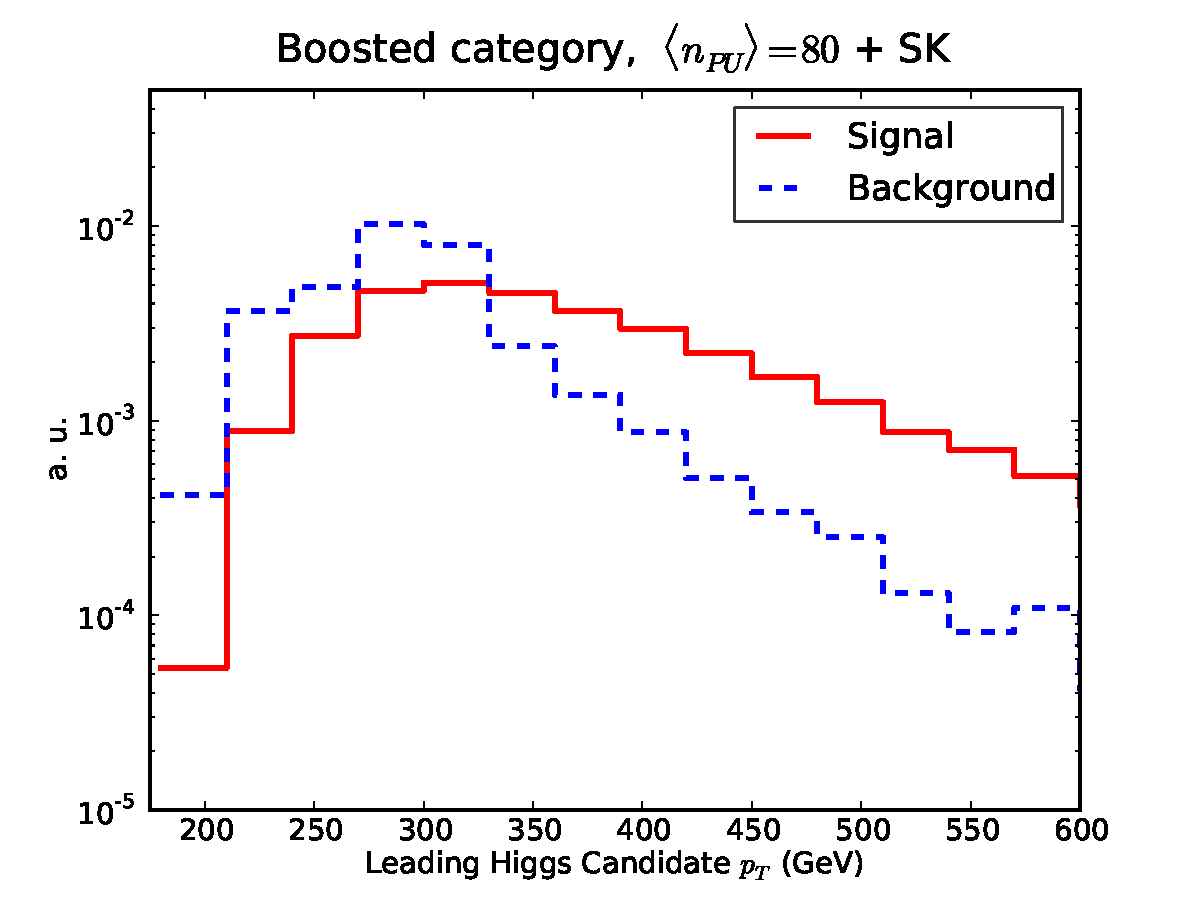
\includegraphics[width=0.49\textwidth]{plots/pt_h0_bst_comp_back.pdf}
   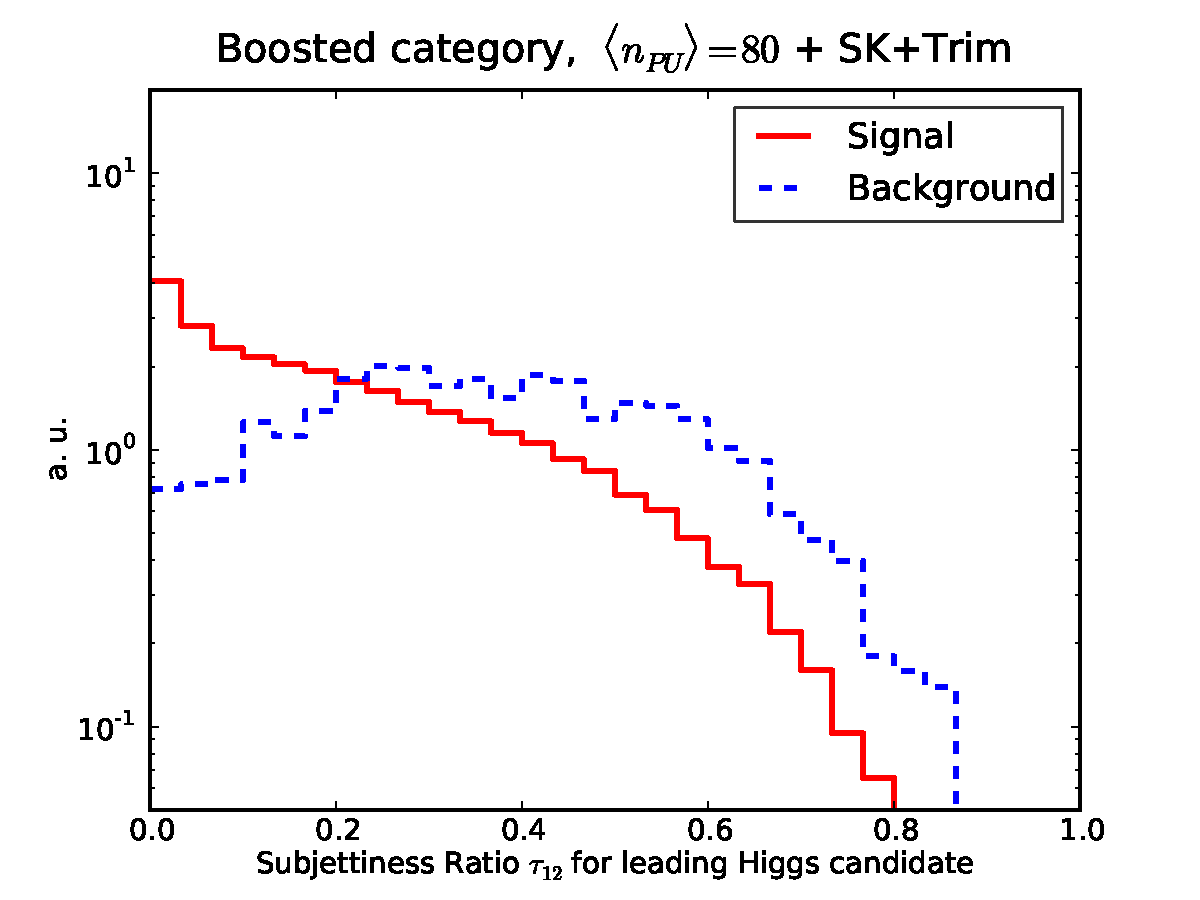
\includegraphics[width=0.49\textwidth]{plots/tau21_h1_bst_comp_back.pdf}
  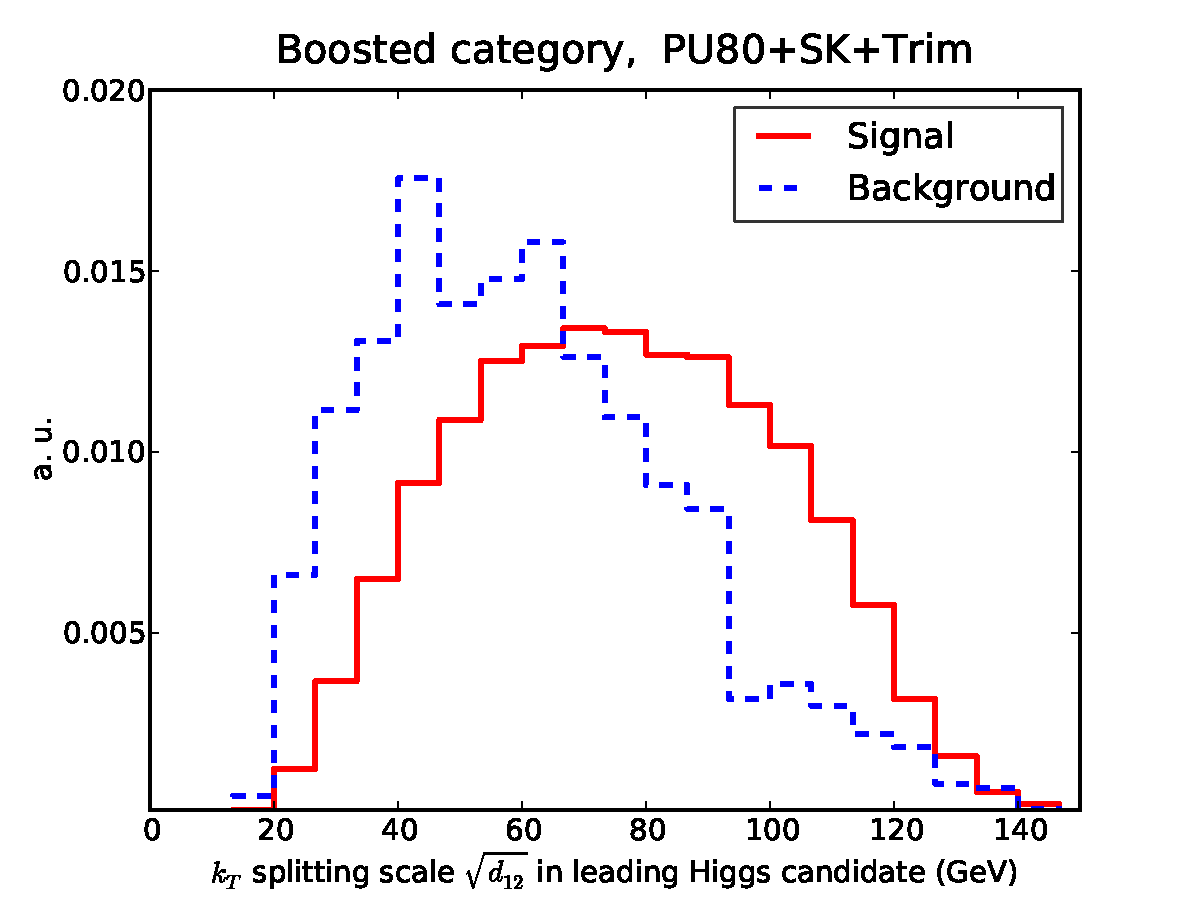
\includegraphics[width=0.49\textwidth]{plots/split12_h0_bst_comp_back.pdf}
   \caption{\small
     Comparison of kinematic distributions, in
     the boosted category, for signal and background events
     with and without PU: the invariant mass,  $p_T$,
     and the substructure variables $\tau_{21}$ and $\sqrt{d_{12}}$
    for the leading Higgs candidate.
     %
 }
\label{fig:signal-vs-back-boosted}
\end{center}
\end{figure}
%%%%%%%%%%%%%%%%%%%%%%%



We can also perform a similar comparison for
the resolved category.
%
In Fig.~\ref{fig:signal-vs-back-resolved} we compare
the kinematic distributions for signal and background events,
     with and without PU, for the invariant mass and the $p_T$ of the leading
     Higgs candidate.
     %
     Also in this
     case the PU-subtracted background distributions appear reasonably close
     to their no PU counterparts.

%%%%%%%%%%%%%%%%%%%%%%%%
\begin{figure}[t]
  \begin{center}
   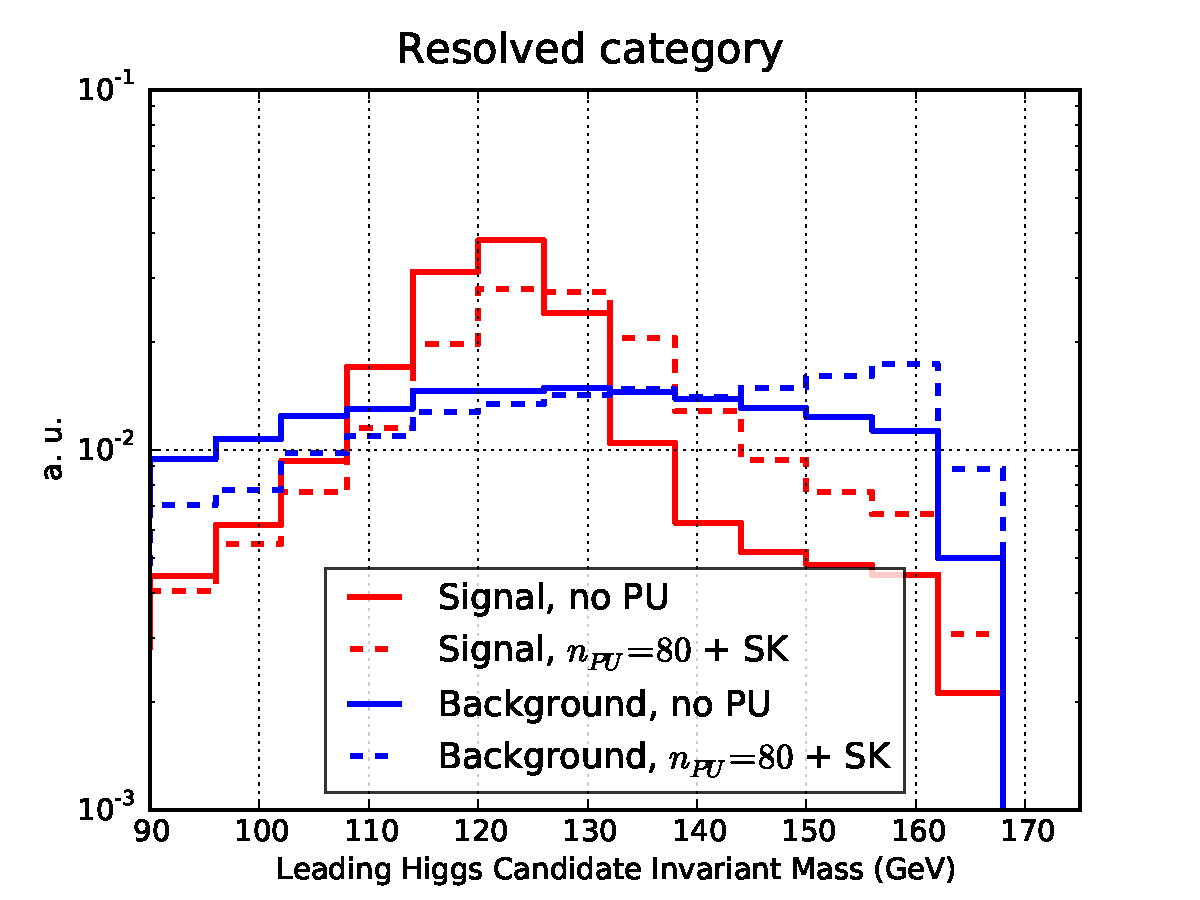
\includegraphics[width=0.49\textwidth]{plots/m_h0_res_comp_back.pdf}
  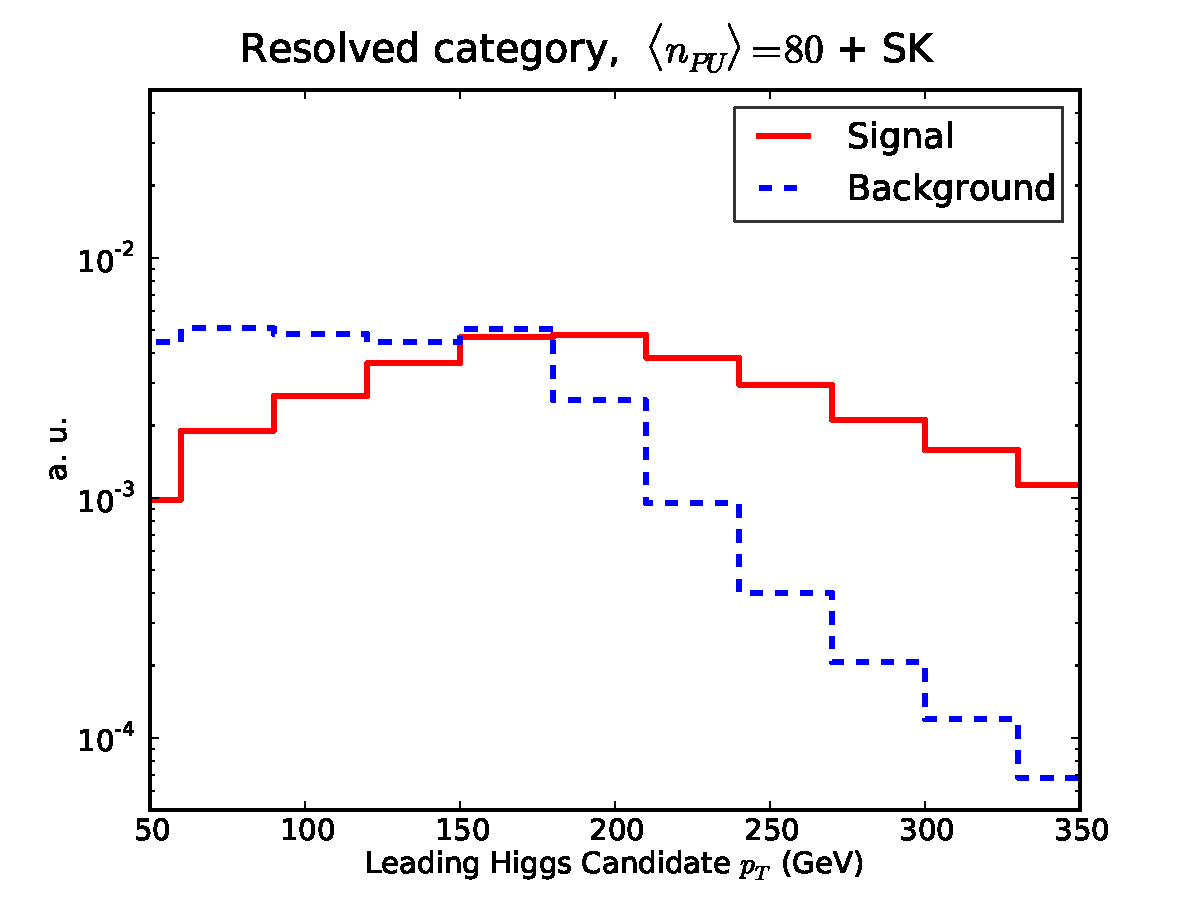
\includegraphics[width=0.49\textwidth]{plots/pt_h0_res_comp_back.pdf}
     \caption{\small
       Same as Fig.~\ref{fig:signal-vs-back-boosted} for the resolved category,
       this time without the jet substructure variables.
}
\label{fig:signal-vs-back-resolved}
\end{center}
\end{figure}
%%%%%%%%%%%%%%%%%%%%%%%

To complete this discussion, it is illustrative to determine
which is the mass resolution obtained for the
reconstructed Higgs candidates in various cases.
%
In Table~\ref{tab:massresolution}
we indicate the shift of the invariant mass peak as compared
to the nominal Higgs mass, $\delta m_h$, as well as the
corresponding width of the distribution, $\sigma_{m_h}$,
obtained from fitting a Gaussian to the mass distributions
of both the leading and subleading Higgs candidates in
the resolved category.
        %
        We show results for three cases: without PU, with PU $\la n_{\rm PU}\ra=80$
        but without subtraction, and the same with SK subtraction.
%
        We find a mass resolution of around 9 GeV in the case
        without PU, which is only slightly degraded
        to around 11 GeV in the case of $\la n_{\rm PU}\ra=80$ PU
        with SK subtraction.
        %
        We also note that, after subtraction, the peak of
        the invariant mass distributions of Higgs candidates
        coincides with the nominal values of $m_h$ within a few GeV.

    %%%%%%%%%%%%%%%%%%%%%%%%%%%%%%%%%%%%%%%%%%%
    \begin{table}[h]
      \centering
      \begin{tabular}{|c|c|c|c|}
        \hline
        &   &   $\delta m_h$  &  $\sigma_{m_h}$  \\
        \hline
        \hline
        \multirow{2}{*}{no PU}  & leading Higgs  &  -3.8 GeV   & 8 GeV   \\
          & subleading Higgs   & -5.8 GeV  &  9 GeV \\
        \hline
          \multirow{2}{*}{$\la n_{\rm PU}\ra=80$}  & leading Higgs  &  +33 GeV   & 9 GeV   \\
          & subleading Higgs   & +31 GeV  &  12 GeV \\
          \hline
            \multirow{2}{*}{$\la n_{\rm PU}\ra=80$+SK}  & leading Higgs  &  +3.9 GeV   & 11 GeV   \\
          & subleading Higgs   & +2.1 GeV  &  11 GeV \\
        \hline
        \end{tabular}
      \caption{\label{tab:massresolution}
        Resolution of the invariant mass distribution of
        reconstructed Higgs candidates in the resolved
        category.
        %
        We show three cases: without PU, with PU $\la n_{\rm PU}\ra=80$
        but without subtraction, and the same with SK subtraction.
        %
        We indicate the shift of the invariant mass peak as compared
        to the nominal Higgs mass, $\delta m_h$, as well as the width
        of a Gaussian fitted to the mass distribution, $\sigma_{m_h}$,
        for both the leading and subleading Higgs candidates.
      }
      \end{table}

%%%%%%%%%%%%%%%%%%%%%%%%%%%%%%%%%%%%%%%%%%%%%%%%%%%%%%%%%%%%
%%%%%%%%%%%%%%%%%%%%%%%%%%%%%%%%%%%%%%%%%%%%%%%%%%%%%%%%%%%%
%%%%%%%%%%%%%%%%%%%%%%%%%%%%%%%%%%%%%%%%%%%%%%%%%%%%%%%%%%%%




%%%%%%%%%%%%%%%%%%%%%%%%%%%%%%%%%%%%%%%%%%%%%%%%%%%
%%%%%%%%%%%%%%%%%%%%%%%%%%%%%%%%%%%%%%%%%%%%%%%%%%%
%%%%%%%%%%%%%%%%%%%%%%%%%%%%%%%%%%%%%%%%%%%%%%%%%%%
%%%%%%%%%%%%%%%%%%%%%%%%%%%%%%%%%%%%%%%%%%%%%%%%%%%

%%%%%%%%%%%%%%%%%%%%%%%%%%%%%%%%%%%%%%%%%%

\section{Results of the cut-based analysis}

\label{sec:results}

In this section we present the results of the 
cut-based analysis, including the corresponding
cut-flow.
We
compare our results with other recent studies,
and in particular
we study how the signal significance
is affected if only the $4b$ component of the
QCD multi-jet background is taken into account,
while the $2b2j$ and $4j$ components are neglected.
%


\subsection{Cut-flow and signal significance}

First of all, we compare the cross-sections at various
analysis levels for the three categories, for signal and background events,
by providing a detailed cut-flow.
%
We consider all backgrounds enumerated in Sect.~\ref{mcgeneration},
and also discuss how results are modified if only the $4b$
component is kept.
%
At each stage of the cut-flow, we also provide the
the signal significance, $S/\sqrt{B}$, and the signal
over background ratio, $S/B$, corresponding to the
 HL-LHC with
an integrated luminosity of $\mathcal{L}
=3000$ fb$^{-1}$.
%
For this type of analysis,
it is crucial not only to achieve a good signal
significance, $S/\sqrt{B}$, but also a good signal over background ratio $S/B$.
%
If the latter is too small, an unrealistically precise
measurement of the background would be required.
%
In Table~\ref{tab:cutflowdetails}
we describe this cut-flow,
separated into the (exclusive) boosted, intermediate,
    and resolved categories.
    %
    From top to bottom, additional cuts are required in addition
    to the previous ones.
    %
    The various cuts
    are defined as follows:

   

%%%%%%%%%%%%%%%%%%%%%%%%%%%%%%%%%%%%%%%%%%%%%%%%%%%%%%%%%%%%%%%%%%%%%%%%%%%%%%%%%%%%%%%%%
%%%%%%%%%%%%%%%%%%%%%%%%%%%%%%%%%%%%%%%%%%%%%%%%%%%%%%%%%%%%%%%%%%%%%%%%%%%%%%%%%%%%%%%%%
\begin{table}[t]
  \centering
  \begin{tabular}{|c|c|c|c|}
\hline
&  Boosted  &   Intermediate &  Resolved  \\
\hline
\hline
{\bf C0} &  \multicolumn{3}{c|}{Generator level} \\
\hline
{\bf C1a} & $N_{\rm jets}^{R10}\ge 2$ & $N_{\rm jets}^{R04}\ge 2$, $N_{\rm jets}^{R10}=1$  &
$N_{\rm jets}^{R04}\ge 4$ \\
\hline
{\bf  C1b} & \multicolumn{3}{c|}{+$p_T$ cuts} \\
{\bf C1c} & \multicolumn{3}{c|}{+rapidity cuts}\\
\hline
 {\bf C1d} & +$N_{\rm MDT}\ge 2$ & +$N_{\rm jets}^{R10}=1$ with MDT  &
 +Higgs reconstruction \\
 \hline
{\bf C1e} & \multicolumn{3}{c|}{ +$m_H$ window cut} \\
\hline
{\bf C2} & \multicolumn{3}{c|}{+$b$-tagging}    \\
\hline
  \end{tabular}
  \caption{\small Cut-flow of the present analysis for the boosted, intermediate
    and resolved selections.
    %
      \label{tab:cutflowdetails}
  }
\end{table}
%%%%%%%%%%%%%%%%%%%%%%%%%%%%%%%%%%%%%%%%%%%%%%%%%%%%%%%%%%%%%%%%%%%%%%%%%%%%%%%%%%%%%%%%%
%%%%%%%%%%%%%%%%%%%%%%%%%%%%%%%%%%%%%%%%%%%%%%%%%%%%%%%%%%%%%%%%%%%%%%%%%%%%%%%%%%%%%%%%%


    \begin{itemize}
    \item {\bf C0}: these are the generator level cross-sections, with
      mild generation cuts in the case of the background processes, and no
      generation cuts
      for the signal events.
      %
    \item {\bf C1a}:  we only check that we have at least
      two large-$R$ jets (in the boosted case),
      one large-$R$ jet and at least 2 small-$R$ jets (in the intermediate
      case) and at least four small-$R$ jets (in the resolved case).
      %
      No acceptance requirements are imposed.
    \item {\bf C1b}: require that the above jets should
      satisfy the corresponding $p_T$ thresholds,
      $p_T \ge 200$ GeV for large-$R$ jets and
      $p_T \ge 50$ GeV for small-$R$ jets.
    \item {\bf C1c}: same for the
      rapidity acceptance requirement.
    \item {\bf C1d}: the two leading large-$R$ jets must
      be mass-drop tagged in the boosted category.
      %
      In the intermediate category, the large-$R$ jet must also be mass-drop tagged.
      %
    \item {\bf C1e}: after the two Higgs candidates  have been reconstructed,
      their invariant masses are required to lie a window around $m_H$,
      in particular between 85 and 165 GeV.
          \item {\bf C2}: finally, the
            $b$-tagging conditions are
            imposed, see
            Sect.~\ref{sec:btagging}.
      \end{itemize}
    Signal and background events satisfying all the analysis cut up to the
    C2 level
    are then used as input for the MVA training, to be described next
    in Sect.~\ref{sec:mva}.

    %
    In Table~\ref{tab:cutflow_noPU_1} we provide
    the values of cross-sections, in femtobarns,
     for the signal
      and the various background
      components as a function of the
      cut-flow, for the resolved,
      boosted and intermediate
      categories.
      %
       In each case, we also provide the signal over
      background ratio, $S/B$, and the signal
      significance, $S/\sqrt{B}$, at the HL-LHC, considering either
      the total background or only the $4b$ component.
     %
      This separation emphasizes
      the  importance of the reducible component of the QCD background.
      %
      Even after $b$-tagging, the reducible $2b2j$ background
      is comparable, or even larger, than the irreducible
      $4b$ component.
      %
      %
      So at the end of the cut-based analysis, signal significance
      are overestimated by up to a factor 2 if the light
      and charm jet background is neglected.

      
    

%%%%%%%%%%%%%%%%%%%%%%%%%%%%%%%%%%%%%%%%%%%%%%%%%
\begin{table}[t]
  \centering
  \scriptsize
  \begin{tabular}{|l|cc|cccc|cccc|}
  \hline
\multicolumn{11}{|c|}{Resolved category, $\la n_{\rm PU}\ra=0$}\\
\hline
&  \multicolumn{6}{c|}{Cross-section [fb]} &  &  & &  \\
   &  $hh\to 4b$ &  total bkg  &   $4b$    &  $2b2j$   &   $4j$    &
$t\bar{t}$ &
$S/B_{\rm tot}$ & $S/B_{\rm 4b}$ & $S/\sqrt{B_{\rm tot}}$ & $S\sqrt{B_{\rm 4b}}$ \\
  \hline
  \hline
 C0    & $39$  &   $5.2\cdot 10^9$   & $1.8\cdot 10^6$ & $3.5\cdot 10^8$ & $4.9\cdot 10^9$ & $3.5\cdot 10^5$  & $7.5\cdot 10^{-9}$   &  $2.2\cdot 10^{-5}$  &   0.03   & 1.6        \\
 C1a   & $39$  &   $5.2\cdot 10^9$   & $1.8\cdot 10^6$ & $3.5\cdot 10^8$ & $4.9\cdot 10^9$ & $3.5\cdot 10^5$ &  $7.5\cdot 10^{-9}$   & $2.2\cdot 10^{-5}$   &     0.03   & 1.6       \\
 C1c   & $22$  &   $2.2\cdot 10^8$   & $6.9\cdot 10^4$ & $1.5\cdot 10^7$ & $2.0\cdot 10^8$ & $2.1\cdot 10^5$ &  $1.0\cdot 10^{-7}$  &  $3.2\cdot 10^{-4}$  &  0.08   & 4.6         \\
 C1d   & $22$  &   $2.2\cdot 10^8$   & $6.9\cdot 10^4$ & $1.5\cdot 10^7$ & $2.0\cdot 10^8$ & $2.1\cdot 10^5$ &  $1.0\cdot 10^{-7}$  & $3.2\cdot 10^{-4}$   &  0.08   & 4.6         \\
 C1e   & $63$  &   $4.4\cdot 10^7$   & $1.6\cdot 10^4$ & $3.2\cdot 10^6$ & $4.1\cdot 10^7$ & $8.8\cdot 10^4$ &   $1.4\cdot 10^{-7}$  &  $3.9\cdot 10^{-4}$   &   0.05   & 2.7         \\
 C2    & $1.2$  &   $4.9\cdot 10^3$   & $1.7\cdot 10^3$ & $2.9\cdot 10^3$ & $2.1\cdot 10^2$ & $47$ &            $ 2.5\cdot 10^{-4}$   & $7.1\cdot 10^{-4}$   &   0.97   & 1.6       \\
\hline
\end{tabular}

  $\,$ \\
  \vspace{0.5cm}
  \begin{tabular}{|l|cc|cccc|cccc|}
  \hline
\multicolumn{11}{|c|}{Intermediate category}\\
\hline
&  \multicolumn{6}{c|}{Cross-section [fb]} &  &  & &  \\
   &  $hh\to 4b$ &  total bkg  &   $4b$    &  $2b2j$   &   $4j$    &
$t\bar{t}$ &
$S/B_{\rm tot}$ & $S/B_{\rm 4b}$ & $S/\sqrt{B_{\rm tot}}$ & $S\sqrt{B_{\rm 4b}}$ \\
  \hline
  \hline
 C0      & 39  &   $5.2\cdot 10^9$   & $1.8\cdot 10^6$ & $3.5\cdot 10^8$ & $4.9\cdot 10^9$ & $3.5\cdot 10^5$ &  $7.5\cdot 10^{-9}$   & $2.2\cdot 10^{-5}$   &   $3.0\cdot 10^{-2}$   & 1.6  \\
 C1c     & 6.9  &   $8.4\cdot 10^7$   & $2.1\cdot 10^4$ & $5.3\cdot 10^6$ & $7.9\cdot 10^7$ & $3.3\cdot 10^4$ &  $8.2\cdot 10^{-8}$   & $3.3\cdot 10^{-4}$ &   $4.1\cdot 10^{-2}$   & 2.6 \\
 C1d     & 6.3  &   $5.8\cdot 10^7$   & $1.4\cdot 10^4$ & $3.6\cdot 10^6$ & $5.5\cdot 10^7$ & $3.0\cdot 10^4$ &  $1.1\cdot 10^{-7}$   & $4.6\cdot 10^{-4}$ &   $4.5\cdot 10^{-2}$   & 2.9\\
 C1e     & 1.3  &   $3.5\cdot 10^6$   & $8.7\cdot 10^2$ & $2.1\cdot 10^5$ & $4.3\cdot 10^7$ & $8.8\cdot 10^3$ &  $3.8\cdot 10^{-7}$   & $1.5\cdot 10^{-3}$  &   $3.9\cdot 10^{-2}$   & 2.5\\
 C2      & 0.22  &   $1.8\cdot 10^2$   & $5.6\cdot 10^1$ & $9.6\cdot 10^1$ & $2.2\cdot 10^1$ & 3.1 & $1.3\cdot 10^{-3}$   & $4.0\cdot 10^{-3}$  &   $9.2\cdot 10^{-1}$   & 1.6 \\
\hline
\end{tabular}

  $\,$ \\
  \vspace{0.5cm}
    \begin{tabular}{|l|cc|cccc|cccc|}
  \hline
\multicolumn{11}{|c|}{Boosted category, $\la n_{\rm PU}\ra=0$}\\
\hline
&  \multicolumn{6}{c|}{Cross-section [fb]} &  &  & &  \\
   &  $hh\to 4b$ &  total bkg  &   $4b$    &  $2b2j$   &   $4j$    &
$t\bar{t}$ &
$S/B_{\rm tot}$ & $S/B_{\rm 4b}$ & $S/\sqrt{B_{\rm tot}}$ & $S\sqrt{B_{\rm 4b}}$ \\
  \hline
  \hline
C0      & 39  &   $5.2\cdot 10^9$   & $1.8\cdot 10^6$ & $3.5\cdot 10^8$ & $4.9\cdot 10^9$ & $3.5\cdot 10^5$  &   $7.5\cdot 10^{-9}$   & $2.2\cdot 10^{-5}$  &  $ 3.0\cdot 10^{-2}$   & 1.6 \\
 C1a     & 39  &   $5.2\cdot 10^9$   & $1.8\cdot 10^6$ & $3.5\cdot 10^8$ & $4.9\cdot 10^9$ & $3.5\cdot 10^5$  &   $7.5\cdot 10^{-9}$   & $2.2\cdot 10^{-5}$ &  $ 3.0\cdot 10^{-2}$   & 1.6  \\
 C1c     & 9.4  &   $4.6\cdot 10^7$   & $1.1\cdot 10^4$ & $2.9\cdot 10^6$ & $4.3\cdot 10^7$ & $2.4\cdot 10^4$ &   $2.0\cdot 10^{-7}$   & $8.3\cdot 10^{-4}$ &  $ 7.6\cdot 10^{-2}$   & 4.8 \\
 C1d     & 6.7  &   $3.7\cdot 10^7$   & $7.5\cdot 10^3$ & $2.1\cdot 10^6$ & $3.5\cdot 10^7$ & $2.2\cdot 10^4$ &   $1.8\cdot 10^{-7}$   & $9.0\cdot 10^{-4}$ &  $ 6.0\cdot 10^{-2}$   & 4.2  \\
 C1e     & 2.5  &   $3.9\cdot 10^6$   & $8.0\cdot 10^2$ & $2.3\cdot 10^5$ & $3.7\cdot 10^6$ & $7.1\cdot 10^3$   &   $6.4\cdot 10^{-7}$   & $3.1\cdot 10^{-3}$ &  $ 6.9\cdot 10^{-2}$   & 4.9\\
 C2      & 0.4  &   $2.5\cdot 10^2$   & $5.3\cdot 10^1$ & $1.9\cdot 10^2$ & $1.3\cdot 10^1$ & 1.6  &   $1.4\cdot 10^{-3}$   & $6.7\cdot 10^{-3}$ &   1.2   & 2.7  \\
\hline
\end{tabular}
%%%%%%%%%%%%%%%%%%%%%%%%%%%%%%%%%%%%%%%%%%%%%%%%%%%%%%%%%%%%%%%

    \caption{\small The cross-sections, in femtobarns,
      for the signal and the various background
      processes at different steps of the
      cut-flow, for the resolved (upper table),
      intermediate (middle table) and boosted
      (lower table) categories, for the analysis
      without PU.
      %
      In each case, we also provide the signal over
      background ratio, $S/B$, and the signal
      significance, $S/\sqrt{B}$, considering either
      the total background or only the $4b$ component.
      %
      The different levels of the cut-flow are summarized
      in Table~\ref{tab:cutflowdetails}.
 \label{tab:cutflow_noPU_1}}
\end{table}
%%%%%%%%%%%%%%%%%%%%%%%%%%%%%%%%%%%%



%
In the boosted category, after all cuts,
one ends
up with more than 1K signal events expected
at the HL-LHC, swamped  however in a almost 1M background events,
leading to $S/\sqrt{B}=1.2$ and $S/B=0.0014$.
%
It should have been possible to somewhat increase this significance
but using more aggressive cuts,
but this is not needed due to the subsequent
optimisation  performed with the MVA.
%
From  Table~\ref{tab:cutflow_noPU_1}
it is also possible to compute the corresponding pre-MVA
expectations for the LHC Run II with
$\mathcal{L}=300$ fb$^{-1}$: one expects
120 signal events, with signal significance dropping down to
$S/\sqrt{B}\sim 0.3$.
%

Both the intermediate and resolved categories benefit from higher signal yields,
specially in the resolved category, but this enhancement is compensated by the
corresponding
increase in the QCD multi-jet background.
%
In both categories
the signal significance is similar to that of the boosted category,
$S\sqrt{B}=0.97(0.92)$ in the resolved
(intermediate) categories,
with the drawback, in the resolved case,
that $S/B$
is one order to magnitude smaller.
%
Combining the pre-MVA results
from the
of the boosted, intermediate and resolved categories,
we obtain a significance for the observation of the Higgs pair production
in the $b\bar{b}b\bar{b}$ final
state at the HL-LHC of  $S/\sqrt{B}=1.8$.

\subsection{The role of light  and charm jet mistags}

One of the main differences of the present study as compared
to previous works is the inclusion of both irreducible
and reducible background components, which allows
to study the impact of the modeling of light and charm jet mistags. 
%
Two recent studies that have also studied the
feasibility of SM Higgs pair production in the $b\bar{b}b\bar{b}$
final state are from the UCL group~\cite{Wardrope:2014kya} and from
the
Durham group~\cite{deLima:2014dta}.
%
The UCL study based
on requiring at least four $b$-tagged $R=0.4$ anti-$k_T$ jets
in central acceptance with $p_T \ge 40$ GeV, which are
then used to construct dijets (Higgs candidates) with
$p_T \ge 150$ GeV, $85 \le m_{\rm dijet} \le 140$ GeV
and $\Delta R \le 1.5$ between the two components
of the dijet.
%
In addition to the basic selection cuts, the discriminating
power of
additional variables is included by means of a 
Boosted Decision Tree (BDT) discriminant.
%
The backgrounds included are the $4b$ and
$2b2c$ QCD multijets, as well as
$t\bar{t}$, $Zh$, $t\bar{t}h$ and $hb\bar{b}$,
and a signal significance of $S/\sqrt{B}=2.1$ for the HL-LHC
is obtained.

The Durham group study~\cite{deLima:2014dta} requires events
to have two $R=1.2$ C/A jets with $p_T\ge 200$ GeV, with
two $b$-tagged subjets inside each large-$R$ jet with
$p_T \ge$ 40 GeV each.
%
To improve the separation between
signal over background separation, both the BDRS
method and the Shower Deconstruction (SD)~\cite{Soper:2011cr,Soper:2012pb}
technique are used.
%
The background considered are QCD $4b$ as well as $Zb\bar{b}$, $hZ$ and
$hW$.
%
At the HL-LHC, the best result is obtained by requiring two
SD-tagged large-$R$ jets, which leads to $S/\sqrt{B}\sim 2.1$, with
 slightly inferior performance with the BDRS tagger.
 %
 

%
 From the results of Table~\ref{tab:cutflow_noPU_1}, we observe
 that the signal significance in the boosted, intermediate,
 and resolved categories is 2.7, 1.6 and 1.6 respectively,
 when only the QCD $4b$ background is included.
 %
 Combining the signal significance in the three categories,
 we
 obtain  a total $S/\sqrt{B_{\rm 4b}}=3.5$, which is a factor
 2 improvement as compared to the result found when
 all background components are included.
 %
 This should be taken into account when comparing
 the results of this work with previous analysis.
 %

 It is interesting to compare in each category the interplay
 between the reducible and irreducible components of the
 QCD backgrounds.
 %
 In the resolved case, the $4b$ and $2b2j$ have a similar
 magnitude, with the latter being larger by a factor of two,
 with $4j$ being smaller by an order of magnitude.
 %
 The situation is similar in the intermediate category, while
 in the boosted category the importance of the $2b2j$ component
 is even more marked, being a factor four larger than the
 $4b$ one.
 %
 Therefore, we conclude that, while the $4j$ component can be safely
 neglected (given the theory uncertainties associated to the
 modelling of the QCD background), the inclusion of the
 $2b2j$ component is essential to robustly assess the feasibility
 of measuring Higgs pairs in this final state.
 %
 This indicates that a promising avenue to improve the prospects
 of this measurement would be to reduce, as much as possible,
 the light and charm jet mistag rate, in addition to achieving
 a higher $b$-tag efficiency.


 In Fig.~\ref{fig:histoBack} we show a
 comparison
    of the shapes of the $4b$ and $2b2j$
components of the QCD background for the $p_T$ of the leading
Higgs candidate in the resolved
and boosted  categories, and the same
 for the invariant
mass $m_{hh}$ of the
    reconstructed di-Higgs system.
    %
    The two components lead to a rather similar shape
    for the two distributions, with some interesting
    differences, for instance in the boosted
    category the $4b$ component is harder for the
    $p_T^h$ distribution, while the $2b2j$ leads to a longer
    tail at small values of the $m_{hh}$ invariant
    mass distribution.
%
    We also observe that the $2b2j$ distributions
    are affected by somewhat larger
    MC fluctuations as compared to $4b$, despite the large size
of the initial sample.
%
This is a consequence of the
difficulties of an accurate modelling of the effects
of $b$-jet mistags from a QCD multi-jets process, requiring
very large MC samples.

%%%%%%%%%%%%%%%%%%%%%%%%%%%%
\begin{figure}[t]
\begin{center}
 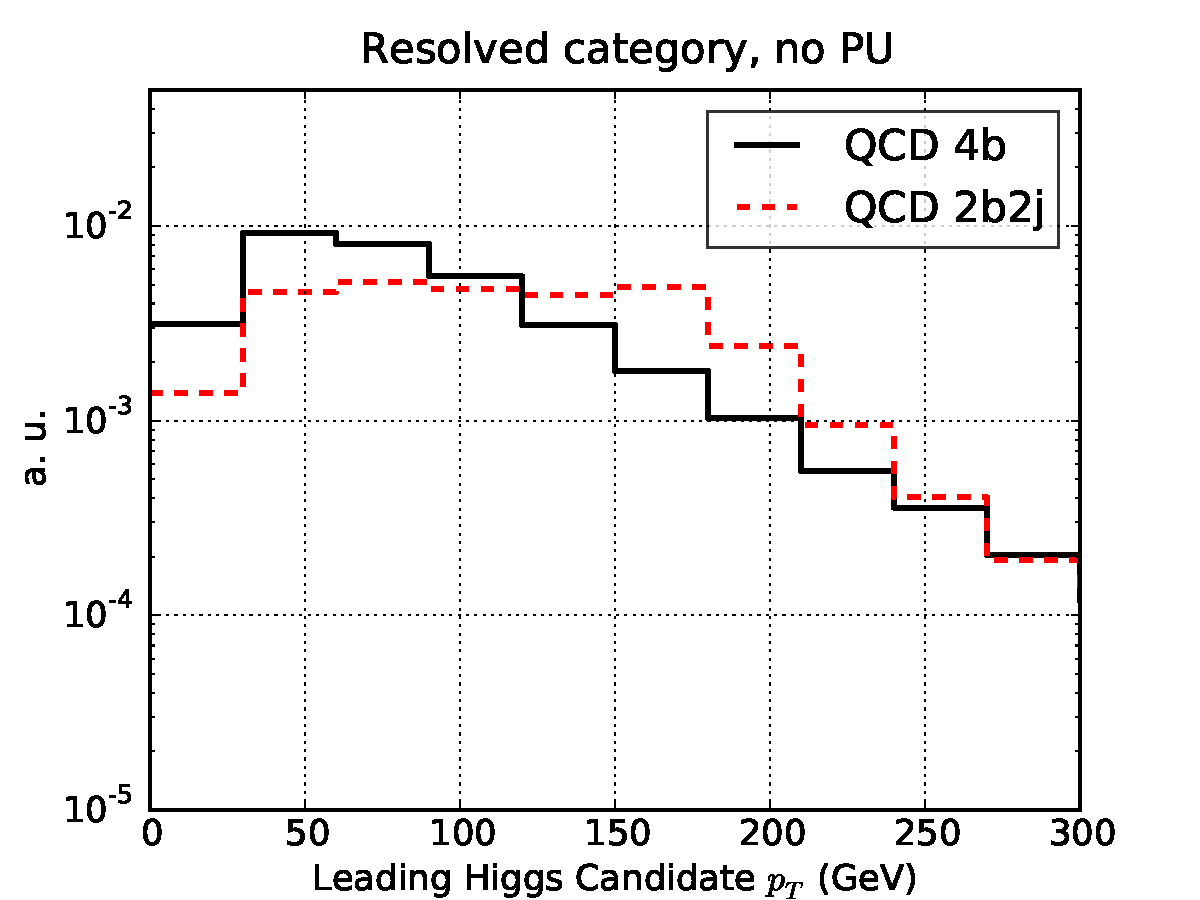
\includegraphics[width=0.49\textwidth]{plots/pt_h0_C2_res_back_noPU.pdf}
 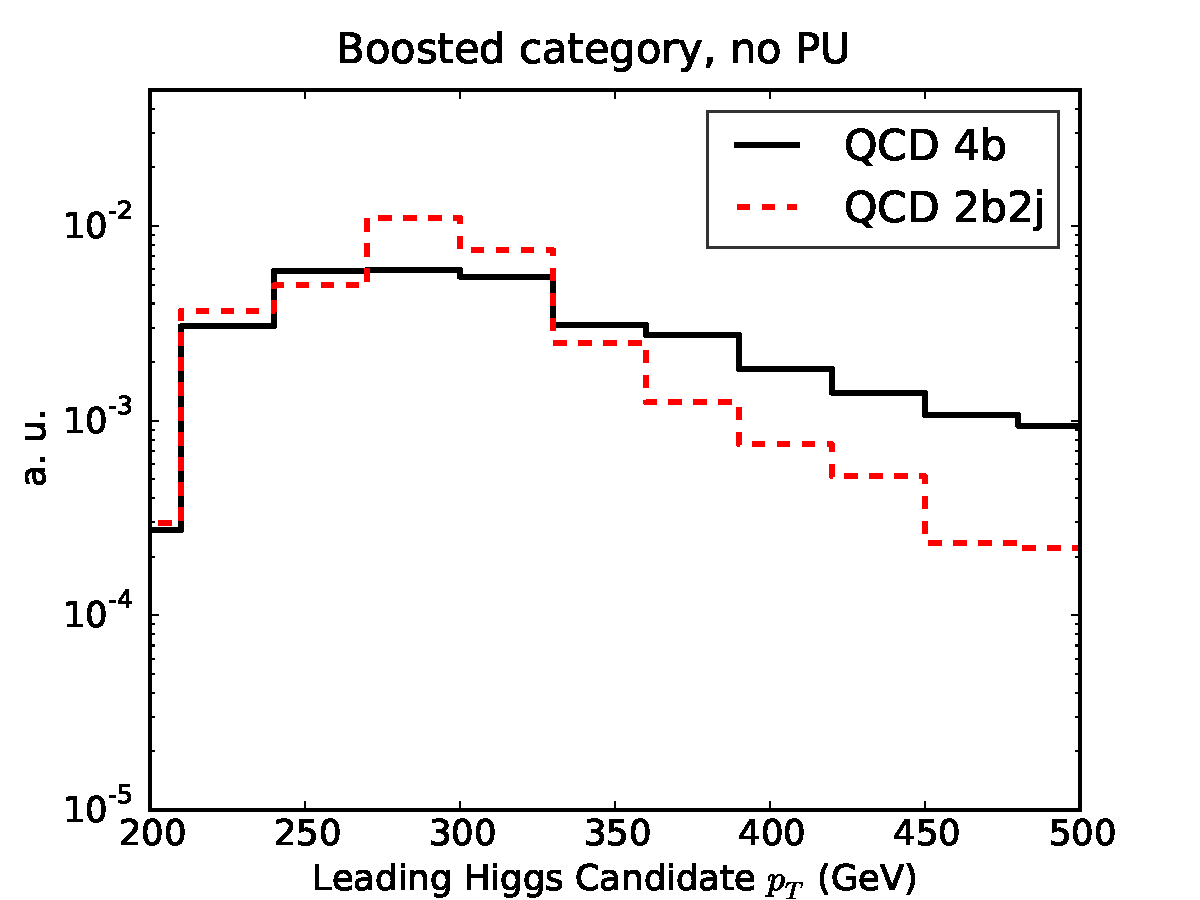
\includegraphics[width=0.49\textwidth]{plots/pt_h0_C2_bst_back_noPU.pdf}
  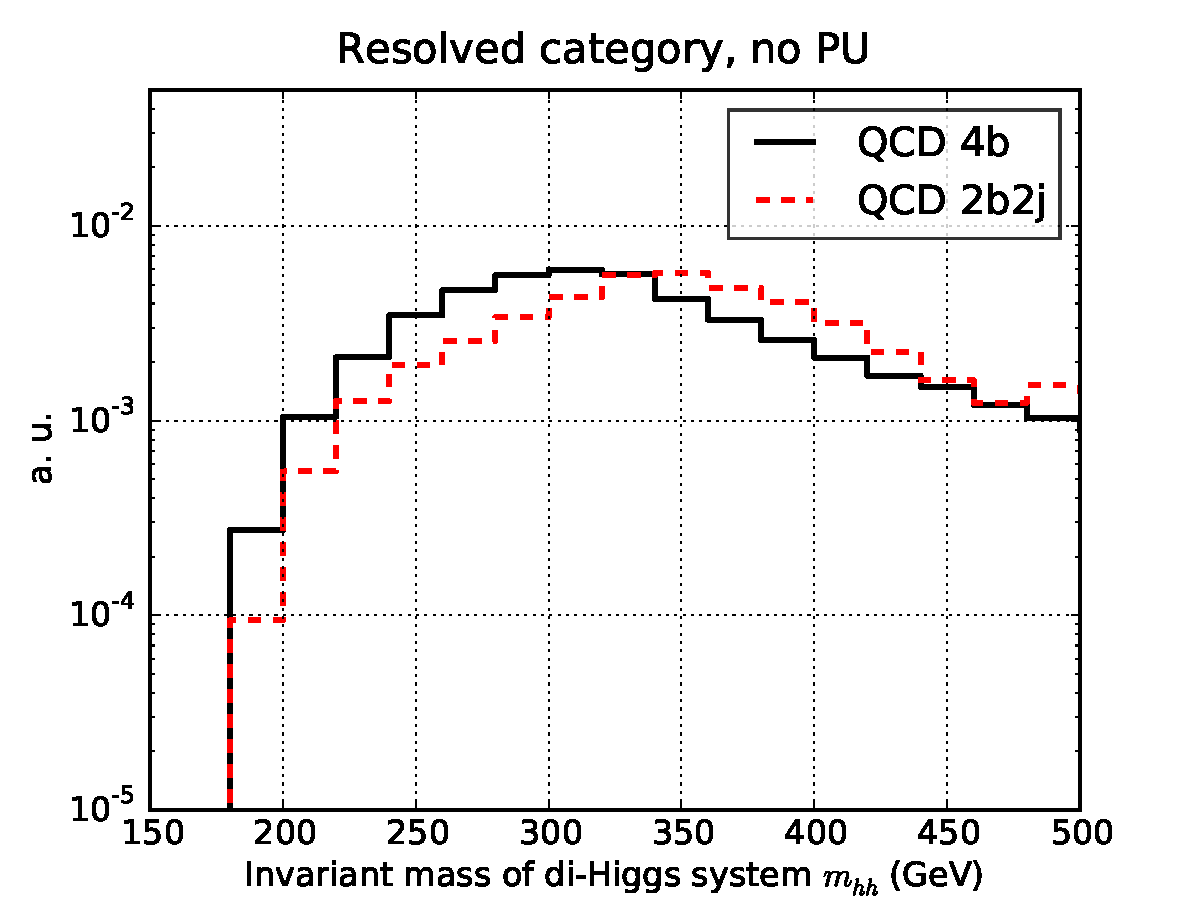
\includegraphics[width=0.49\textwidth]{plots/m_hh_C2_res_back_noPU.pdf}
  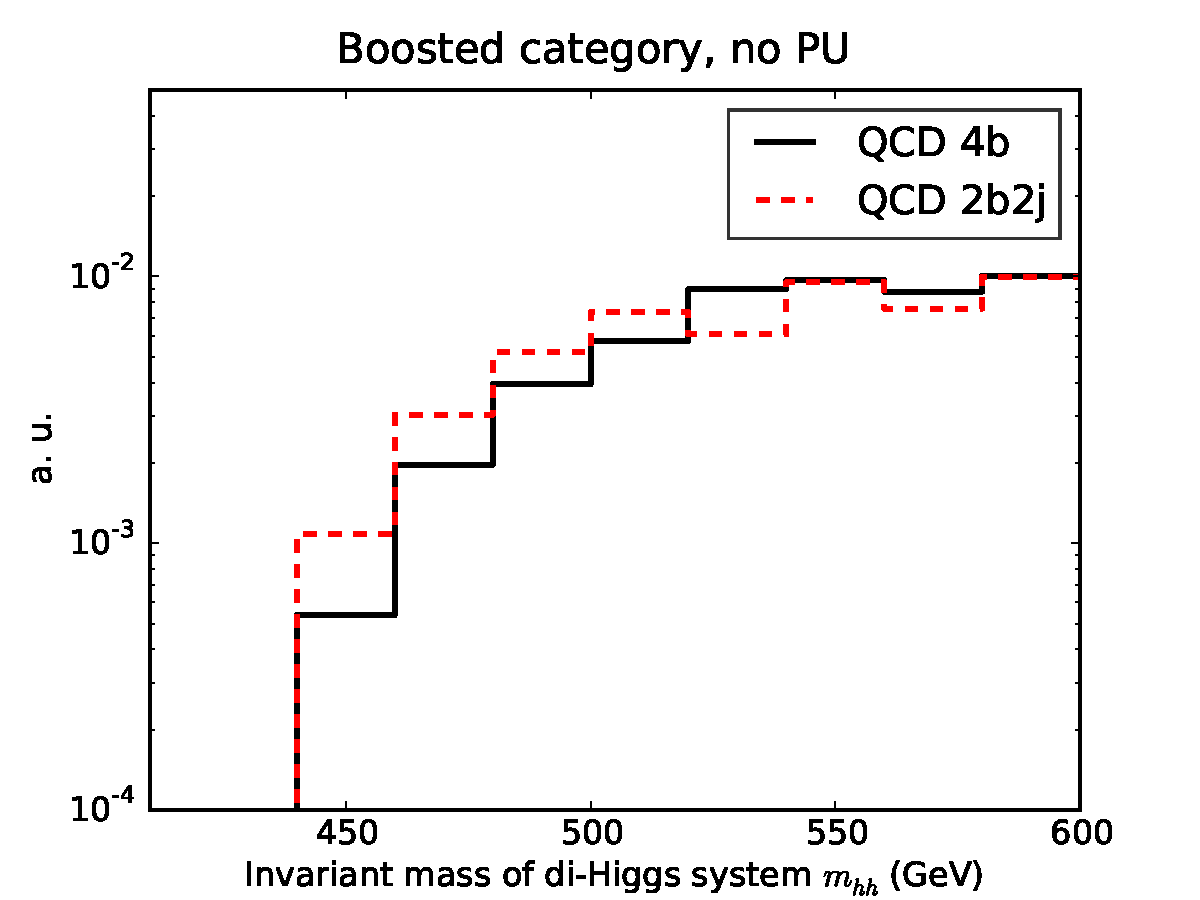
\includegraphics[width=0.49\textwidth]{plots/m_hh_C2_bst_back_noPU.pdf}
  \caption{\small
    Upper plots: comparison
    of the shapes of the $4b$ and $2b2j$
components of the QCD background for the $p_T$ of the leading
Higgs candidate in the resolved
(left plot) and boosted (right plot) categories.
    %
Lower plots: the same comparison this time for the invariant
mass $m_{hh}$ of the
    reconstructed di-Higgs system.
}
\label{fig:histoBack}
\end{center}
\end{figure}
%%%%%%%%%%%%%%%%%%%%%%%

The reason why the  $2b2j$ process
is not negligible as compared to the $4b$ component
is the following.
%
In the boosted category, for example,
the cross-sections at the C1e
level, that is, after the mass-drop tagging but before
$b$-tagging, is a factor 300 larger in the $2b2j$
sample as compared to the $4b$ sample.
%
Now, after $b$-tagging, the naive expectation would
be a suppression of the former by a factor $f_l^2/f_b^2 =3\cdot 10^{-4}$,
since a total of four $b$-tags are required to classify the
event as a Higgs candidate.
%
So the ratio of $2b2j$ over $4b$ should be
around $\simeq 3\%$.
  %
While  we have checked that this expectation is borne
out at parton level, before showering,
we find that  when parton shower effects
are accounted for, due to the radiation of $b\bar{b}$ pairs from the
light jets as well as due to combinatorics, the
number of  $b$ quarks in the  final state is
increased substantially in the $2b2j$ component as compared
to the parton level content,
enhancing the signal efficiency and making
it comparable to the $4b$ component.


We can make this statement more quantitative in the following way.
%
To first approximation, and neglecting the contribution from charm mistags, the
overall efficiency of the $b$-tagging requirements in the resolved category will be
given by the following expression:
\be
\label{btaggingeff}
{\rm EFF}_{\rm b-tag}\simeq \sum_{j=0}^{4}n^{\rm (b-jet)}_j\cdot f_b^{j}\cdot f_l^{4-j} \, ,
\ee
with $n^{\rm (b-jet)}_j$ the fraction of events, satisfying all the selection cuts,
where $j$ jets, out of the leading four jets, of the event contain $b$ quarks (with $p_T^b\ge 15$
GeV).
%
Similar expressions can be derived to the boosted and intermediate categories.
%
The naive expectation is that all events in the $4b$ sample have $n^{\rm (b-jet)}_4\simeq 1$
and $n^{\rm (b-jet)}_j\simeq 0$ for $j\ne 4$, while the events in the $2b2j$ sample
should have $n^{\rm (b-jet)}_2\simeq 1$ and zero otherwise.
%
This leads to a ratio of overall $b$-tagging selection efficiencies
\be
\label{eq:naive}
\frac{ {\rm EFF}_{\rm b-tag} \lc 2b2j \rc}{{\rm EFF}_{\rm b-tag} \lc 4b\rc}
  \simeq
 \lp \frac{f_l}{f_b}\rp^2 \simeq 1.6\cdot 10^{-4} \, .
\ee
However, the actual situation is more complicated.
%
First of all, we will have a non-negligible fractions $n^{\rm (b-jet)}_j$
with $j=3,4$ also in the $2b2j$ sample, due to $b$-quark pair radiation
during the shower.
%
Secondly, not all events in the $4b$ sample will lead to four small-$R$ $b$-jets,
due to a combination of selection cuts and
parton shower effects.
%

%%%%%%%%%%%%%%%%%%%%%%%%%%%%%%%%%%%%%%%%%%%%%%%%
\begin{table}[t]
  \centering
  \small
  \begin{tabular}{|c|c|c|c|c|c|c|c|}
    \hline
  \multicolumn{2}{|c|}{}   &  $n^{\rm (b-jet)}_0$  &  $n^{\rm (b-jet)}_1$  &  $n^{\rm (b-jet)}_2$  & $n^{\rm (b-jet)}_3$ &
    $n^{\rm (b-jet)}_4$ & ${\rm EFF}_{\rm b-tag}$ \\
    \hline
    \hline
    Signal  &  $hh\to 4b$  &   0.1\%    & 3\%     &  25\%     & 53\%     & 20\%      & 8.5\%  \\
    \hline
    \multirow{3}{*}{Background}  &  QCD $4b$  & 1\%      &  8\%    &   27\%   &  44\%     & 20\%       &  8.4\% \\
     &  QCD $2b2j$  &   9\%    & 42\%     &  49\%    & 1\%     &  0.1\%     & 0.04\%  \\
    &  QCD $4j$  &   96\%    &  3.5\%     & 0.5\%     &  0.01\%    & $3\cdot 10^{-4}$\%      &
    $2\cdot 10^{-4}$\%\\
    \hline
  \end{tabular}
  \caption{\small
    The relative fractions  $n^{\rm (b-jet)}_j$ of events for the resolved selection
    for which, out of the four leading small-$R$ jets, $j$ jets
    contain at least one $b$-quark with $p_T^b\ge 15$ GeV,
    both for signal events and for the three QCD background samples.
    %
    The last column indicates the overall predicted
    selection efficiency of the $b$-tagging procedure,
    Eq.~(\ref{btaggingeff})
    \label{tab:btaggingcheck}
  }
  \end{table}
%%%%%%%%%%%%%%%%%%%%%%%%%%%%%%%%%%%%%%%%%%%%%%%

In Table~\ref{tab:btaggingcheck} we collect
the values of $n^{\rm (b-jet)}_j$ for the signal and the three QCD background samples.
%
Therefore, we find that, rather than the estimate Eq.~(\ref{eq:naive}),
the correct ratio of $b$-tagging selection efficiencies is instead
\be
\frac{{\rm EFF}_{\rm b-tag} \lc 2b2j\rc}{{\rm EFF}_{\rm b-tag} \lc 4b\rc}=
  \frac{0.04\%}{8.4\%} \simeq 5\cdot 10^{-3} \, .
  \ee
  This suppression factor is of the same order of the ratio of $4b$ to $2b2j$ cross-sections
  in the resolved category before $b$-tagging, see Table~\ref{tab:cutflow_noPU_1}.
    %
    This explains why the $2b2j$ contribution cannot be neglected as compared
    to the irreducible $4b$ component of the QCD background.
    %
    A similar calculation from the numbers of Table~\ref{tab:btaggingcheck} shows
    that, on the other hand, the $4j$ component of the background can safely
    be neglected.
    






%


\section{Multivariate analysis}
\label{sec:mva}

At the end of the cut-based analysis,
combining the three categories,
we obtain a signal significance of $S/\sqrt{B}\simeq 1.7 (3.5)$
with all backgrounds (only QCD $4b$) taken into account.
%
We now show how this signal significance
 can be enhanced when the cut-based analysis
 is complemented with a multivariate analysis (MVA).
%
 Multivariate techniques are by now a mature tool
 in high-energy physics data analysis, opening
 new avenues for improving the performance
of many measurements and searches at high-energy colliders.
%
In particular, the classification of events between signal and
background processes by means of MVAs is a
commonly applied strategy in LHC
applications~\cite{Baldi:2014pta,Aaltonen:2012qt,
  Wardrope:2014kya,Chatrchyan:2013zna,Dall'Osso:2015aia}.

In this section, first of all we present the specific MVA that we use,
based on feed-forward multi-layer neural networks.
%
We then introduce the input variables that are
used the MVA, including the jet substructure
variables, and then present the results of $S/\sqrt{B}$ including
the MVA effects.
%
Since we find that jet substructure variables are a crucial input
to the MVA, we show representative kinematic distributions
for these variables.
%
Finally, we assess the robustness of the MVA strategy in
high-PU environments.

\subsection{Deep artificial neural networks}

%
The specific type of  MVA that we use to
disentangle signal and background events is
a multi-layer feed-forward artificial neural network (ANN),
known as a {\it perceptron}.\footnote{This type of ANNs are the same
  as those used to parametrize Parton Distribution Functions
in the NNPDF global analyses~\cite{DelDebbio:2004qj,Ball:2008by,Ball:2011mu,Ball:2010de}.}
%
This family of ANNs is also known as {\it deep} neural networks, since they have
a richer architecture with hidden layers.
%
The input to the MVA are the
signal and background
events which satisfy the requirements of the
cut-based analysis.
%
The output of the trained ANNs allows the identification, in a fully automated way,
of the most relevant variables to discriminate between 
signal and background.

In this work, the ANN that we use has the following architecture.
\be
\label{eq:nn1}
N_{\mathrm{var}}\times5\times3\times1 \, ,
\ee
where $N_{\mathrm{var}}$ represents the number of input variables for the MVA,
which is different in the resolved, intermediate, and boosted categories.
%
All neural-network layers use a sigmoid activation function, allowing
for a probabilistic
interpretation of the ANN output.
%
In Fig.~\ref{fig:nnarch} we show an illustrative
example of a ANN used in this work, corresponding 
to the case of the boosted category (thus $N_{\mathrm{var}}=21$, as we explain below).

%%%%%%%%%%%%%%%%%%%%%%%%
\begin{figure}[t]
  \begin{center}
      \vspace{-1cm}
  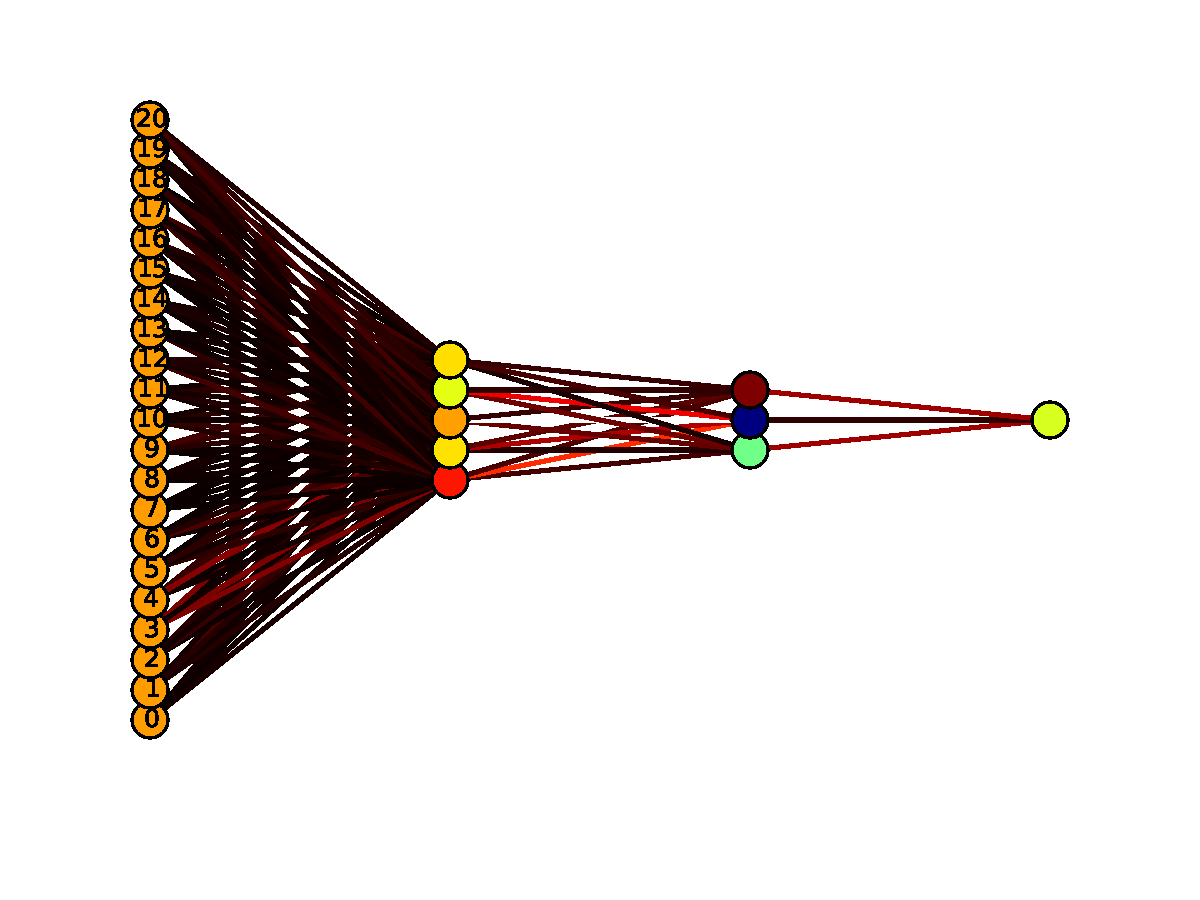
\includegraphics[width=0.90\textwidth]{plots/bst_nnarch_noPU.pdf}
  \vspace{-2cm}
  \caption{\small Architecture of the Artificial
    Neural Network (ANN)
    used for the analysis of the
    boosted
    category, with $N_{\rm var}=21$ input variables and thus
    the same number of neurons
  in the first layer.
  %
  The color code in the neuron connections (the weights) is a heat map obtained
  at the end of the GA training,
  with red indicating larger values and black smaller values.
}
\label{fig:nnarch}
\end{center}
\end{figure}
%%%%%%%%%%%%%%%%%%%%%%%

The training of the ANN for the signal/background classification task
proceeds as follows.
%
Given a set of $N_{\mathrm{var}}$  kinematic variables $\{k\}_i$ associated with the event $i$, and a set of neural network weight
parameters $\{\omega\}$, we interpret the neural network output $y_i$
(the activation state of the
neuron in the last layer)
as the probability that the event $i$ originates from the signal process,
\be
y_i = P(y^\prime_i=1|\{k\}_i, \{\omega\} )\, ,
\ee
where $y_i^\prime$ represents the true classification of the event $i$, {\it i.e},
$y^\prime = 1$ for signal and $y^\prime = 0$ for background events.
%
With this interpretation, our general classification probability including background events is given by
\be
P(y_i^\prime|\{k\}_i, \{\omega\}) = y_i^{y^\prime_i}(1-y_i)^{1-y^\prime_i} \, ,
\ee
which implies that the  error function $E(\{\omega\})$
that needs to be minimized during the ANN training is 
the cross-entropy function, defined as
 \bea
 &&E(\{\omega\}) \equiv -\log\left(\prod_i^{N_{\text{ev}}} P(y_i^\prime|\{k\}_i, \{\omega\})\right)\nonumber\\
 &&=
 \sum_i^{N_{\text{ev}}} \lc y^\prime_i\log{y_i} + (1-y^\prime_i)\log{(1-y_i)}\rc \, ,
 \label{cross-entropy}
 \eea
 where $N_{\text{ev}}$ is the number of
 Monte Carlo events that are used for the ANN training.
 %
 The ANN is trained both on the signal and background MC events,
 so it is crucial to ensure that the input MC sample is large enough
 to avoid the contamination from MC statistical fluctuations.

 
 The training of the neural networks thus consist on the
 minimization of the cross-entropy error,
 Eq.~(\ref{cross-entropy}), which in this work is achieved using a
 Genetic Algorithm (GA).
 %
 Genetic Algorithms~\cite{quevedo,tau,Abel:2014xta,Nesseris:2012tt} are
 non-deterministic
 minimization strategies suitable for the solution
 of complex optimization problems, for instance when a very large number
 of quasi-equivalent minima are present.
 %
 GAs are inspired on natural selection processes
 that emulate biological evolution. 
 %
 In our case, the GA training is performed for a very large 
 number of generations, $N_{\rm gen}=5\cdot 10^{4}$, to avoid the risk of
 under-training.
 %
 We have verified that if a much larger number of generations
 are used, the results are unchanged.
 %

 In order to avoid over-fitting,
 we have used a cross-validation stopping
 criterion, in particular the same one as
 that used in the NNPDF3.0 analysis~\cite{Ball:2014uwa}.
 %
 This cross-validation entails dividing the input MC dataset into two disjoint sets,
 and use one for the training and the other for the validation: the optimal
 stopping point is then indicated by the minimum of the error function
 Eq.~(\ref{cross-entropy}) for the validation sub-sample.
 %
 This indicates the point where we are training on the statistical fluctuations
 of the input MC samples, rather than in the underlying (smooth) physical
 distributions.
 

 \subsection{Input kinematical variables}
 \label{sec:input}

 To ensure that we include the variables with higher discriminatory power,
 we need to train
 the MVA on a large number of kinematic distributions.
%
In this work we use different sets of
input variables for the three categories.
%
In particular, in the case of large-$R$ jets (for the boosted
and intermediate categories), we are fully exploiting the jet
substructure information.

For the three categories, boosted, intermediate and resolved,
the following common variables are used as input to the MVA:
\begin{itemize}
\item The transverse momenta of the leading and subleading Higgs, $p_{T,h_1}$ and $p_{T,h_2}$.
\item The transverse momentum of the reconstructed Higgs pair, $p_{T,hh}$.
\item The invariant masses of the leading and sub-leading Higgs candidates, $m_{h,1}$ and $m_{h,2}$.
\item The invariant mass of the reconstructed Higgs pair, $m_{hh}$.
\item The separation in the $\phi$--$\eta$ plane
  between the two Higgs candidates, $\Delta R_{hh}$.
  \item The separation in $\eta$  between the two Higgs candidates, $\Delta \eta_{hh}$.
\item The separation in $\phi$  between the two Higgs candidates, $\Delta \phi_{hh}$.
\end{itemize}
In addition, in the boosted category we use
  the transverse momenta of the leading, $p_{T,h_{1,1}}$ and $p_{T,h_{1,2}}$ and
  sub-leading, $p_{T,h_{2,1}}$ and $p_{T,h_{2,2}}$, Higgs candidate AKT03 subjets.
  %
  In the resolved category instead,
  the corresponding variables are
  the transverse momenta $p_{T,i}$ of the four leading 
  $b$-tagged small-$R$ jets in the event.
  %
  In the intermediate category, we use the
  transverse momenta of the subjets
  from the large-$R$ jet $p_{T,h_{1,1}}$ and $p_{T,h_{1,2}}$ and the
 transverse momenta $p_{T,i}$ of the two leading 
  $b$-tagged small-$R$ jets.
  %
 Therefore, we have 13 variables which are common to the three categories.

 In the boosted and intermediate categories, we also include the jet substructure
 variables introduced in Sect.~\ref{sec:analysis} for the
 large-$R$ jets: the $k_t$ splitting scales
 $\sqrt{d_{12}}$, the ratio of 2-to-1 subjettiness $\tau_{12}$,
 and the ratios of energy correlation functions $C^{(\beta)}_2$ and
 $D_2^{(\beta)}$.
 %
 Therefore, we end up with
 a total of $N_{\mathrm{var}}=13,17$ and 21 variables for the
resolved, intermediate, and boosted categories, respectively.


Given that the MVA is able to identify the most discriminatory variables
in an automated way,
and to ignore those that have little effect, it is advantageous to
include as many input variables as possible.
%
This is one of the main advantages of ANNs in this context: they are
inherently redundant, so
adding additional information, even if carries very little weight,
should not degrade
the classification power of the MVA, other than making the GA
minimization somewhat less efficient.

\subsection{MVA results}
\label{sec:signalsignificance}

We now present the results of the MVA, first without PU, and then
later including the effects of PU.
%
First of all, in Fig.~\ref{fig:nnresponse} we show the distribution of
the ANN output at the end of the GA minimization, for the exclusive
boosted, intermediate and resolved categories.
%
All distributions are normalized so that their integral
  adds up to one.
%
The  separation between signal and background is achieved by introducing
a cut, $y_{\rm cut}$, on the ANN output, so that MC events with $y_i\ge
y_{\rm cut}$ are classified as signal events, and those with
 $y_i <
y_{\rm cut}$ as background events.
%
Therefore,
the more differentiated is the distribution of the ANN output
for signal and background events, the more efficient
the MVA discrimination will be.

%%%%%%%%%%%%%%%%%%%%%%%%%%%%
\begin{figure}[t]
\begin{center}
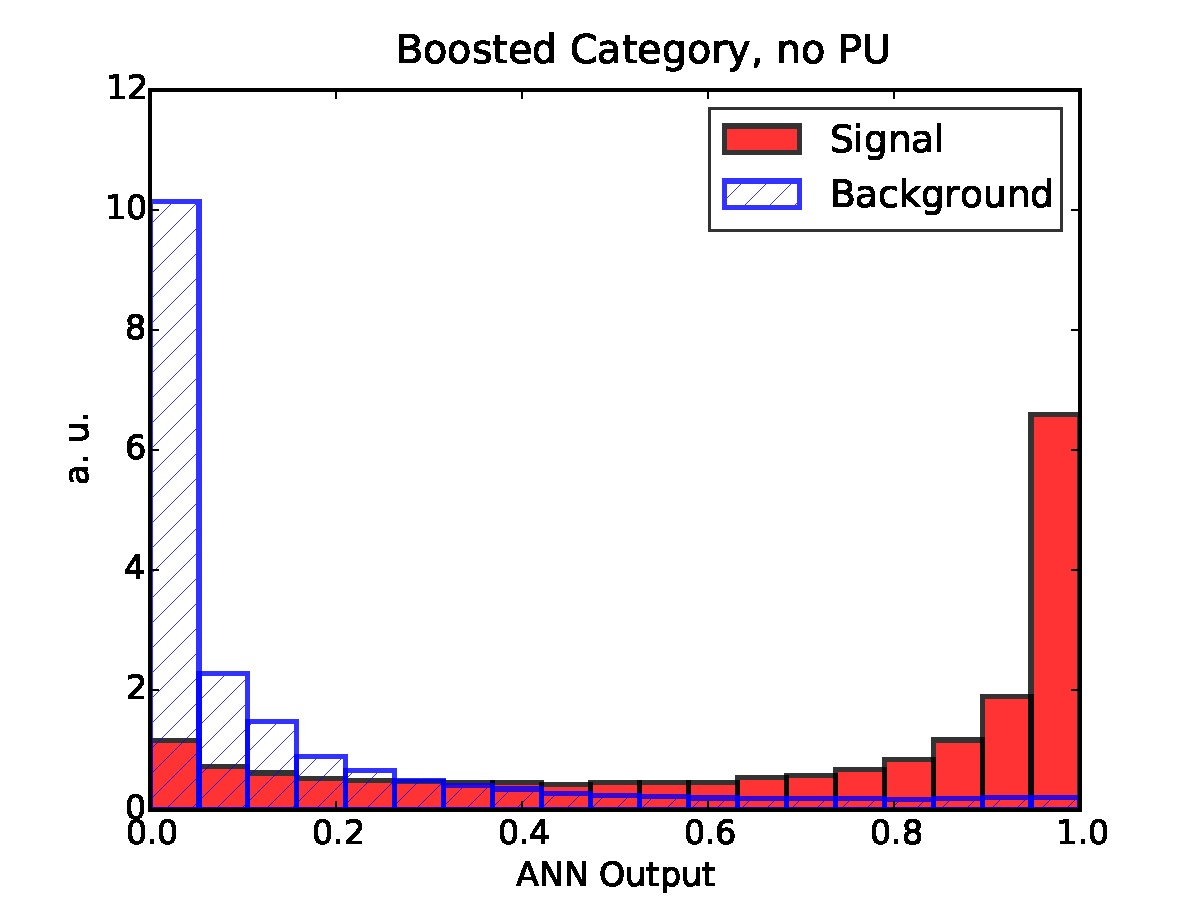
\includegraphics[width=0.65\textwidth]{plots/Boosted_disc_noPU.pdf}
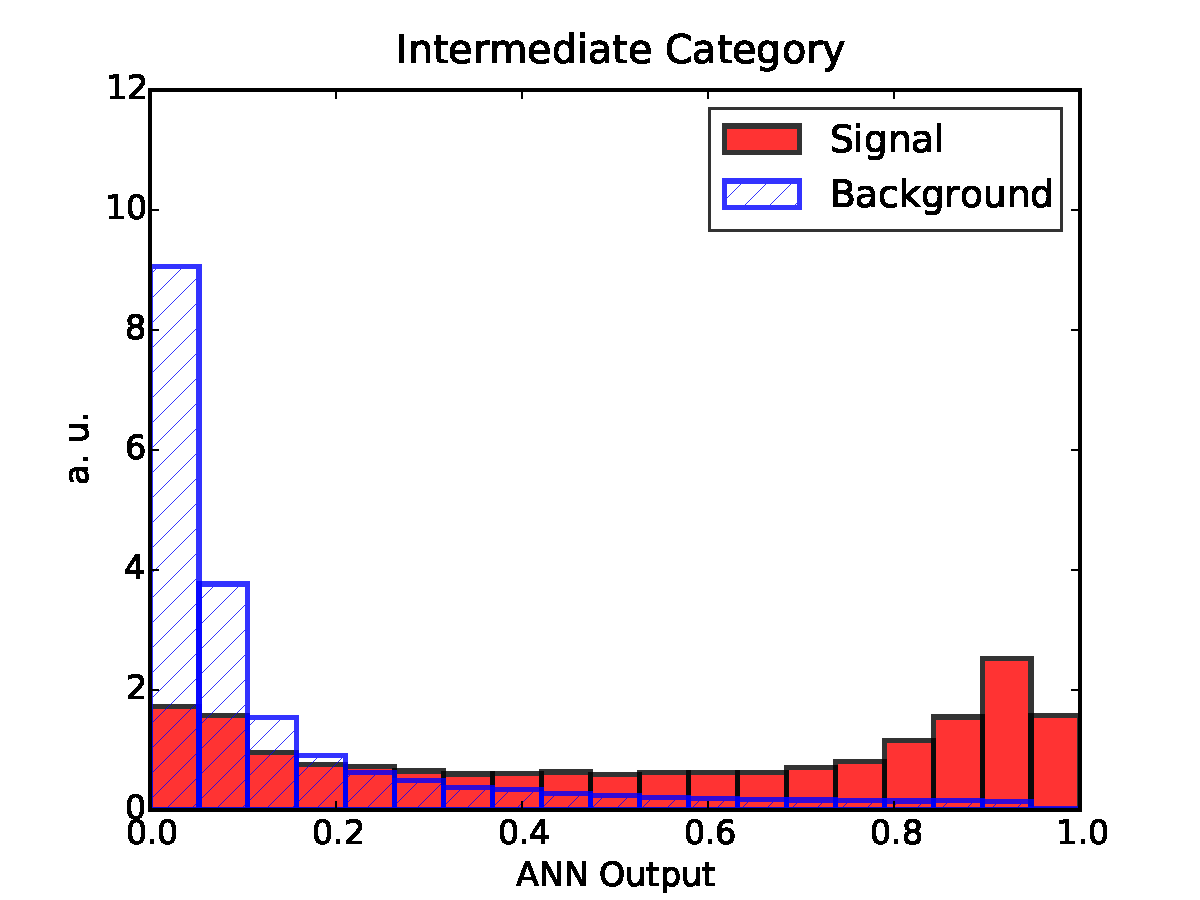
\includegraphics[width=0.48\textwidth]{plots/Intermediate_disc_noPU.pdf}
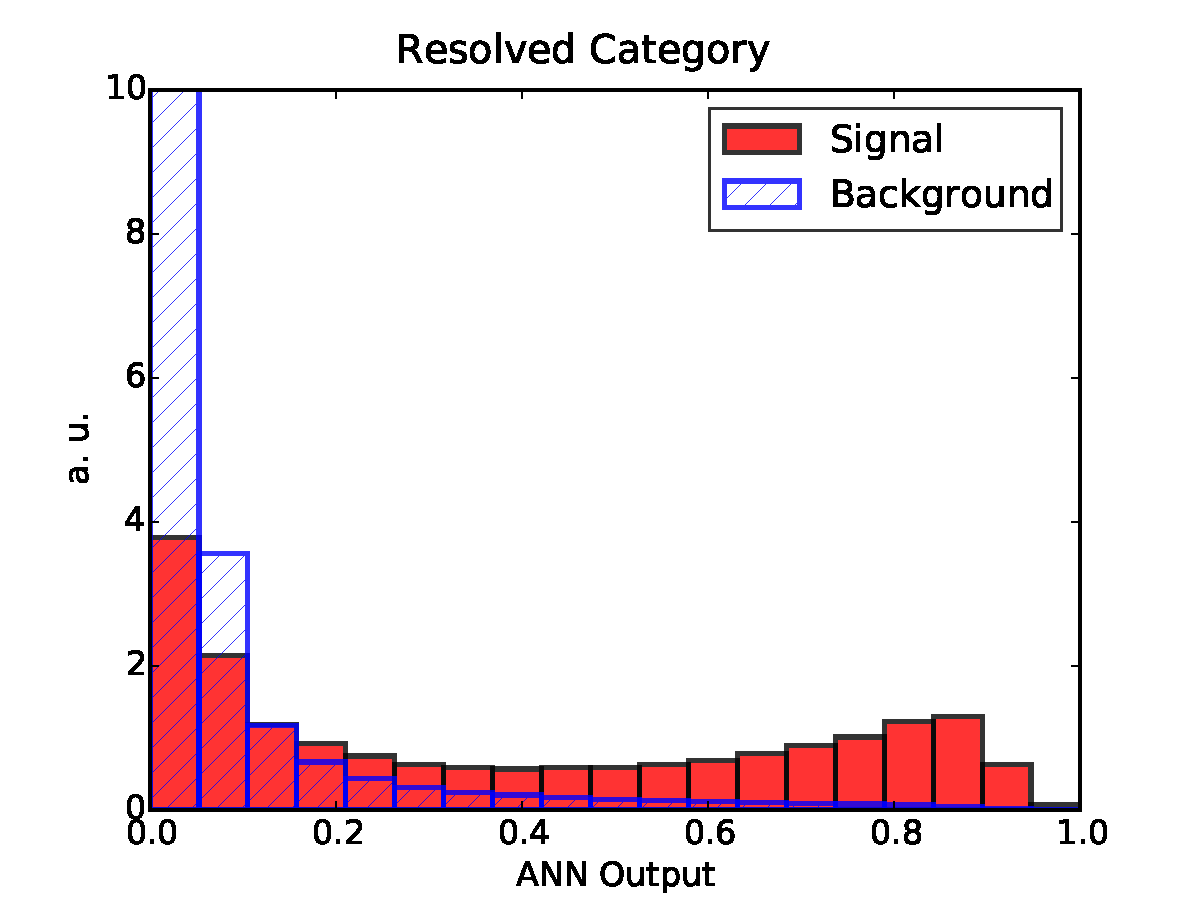
\includegraphics[width=0.48\textwidth]{plots/Resolved_disc_noPU.pdf}
\caption{\small The distributions, at the end of the
  GA training, 
  for the signal and background MC events in the three categories:
  boosted (upper plot), intermediate (lower left plot) and
  resolved (lower right plot), as a function of the ANN output.
}
\label{fig:nnresponse}
\end{center}
\end{figure}
%%%%%%%%%%%%%%%%%%%%%%%

From Fig.~\ref{fig:nnresponse} we see that in the boosted category the MVA manages
to achieve a clear discrimination between signal and background, with the two distributions
nicely peaking at 1 and at 0 respectively.
%
This indicates that introducing a suitable cut
$y_{\rm cut}$
in the ANN output will substantially reduce the background,
while keeping a reasonable signal efficiency.
%
The performance of the MVA discrimination is similar though slightly worse in the intermediate
and resolved categories.
%
The results for the signal selection efficiency and the 
background rejection rate as a function of the cut in the ANN output
$y_{\rm cut}$
define the so-called  Receiver-Operating Characteristic (ROC)
curve, shown in Fig.~\ref{fig:exampleroc}.
%
It is clear that we can achieve  high signal efficiency by using
a small value of $y_{\rm cut}$, but this choice will be
affected from a poor background
rejection.
%
Conversely, using a higher value of the cut will increase background rejection at the
cost of dropping signal efficiency.
%
As could already be inferred from the distribution of neural
networks output in Fig.~\ref{fig:nnresponse}, we find
that our MVA is reasonably efficient
in discriminating signal over background.
%
The performance is best in the case of the boosted category,
and then slightly worse in the resolved
and intermediate categories, consistent with the distributions of
the ANN outputs from
Fig.~\ref{fig:nnresponse}.
%

%%%%%%%%%%%%%%%%%%%%%%%%%%%%%%%%%%%%%%%%%%%%%%
\begin{figure}[t]
\begin{center}
  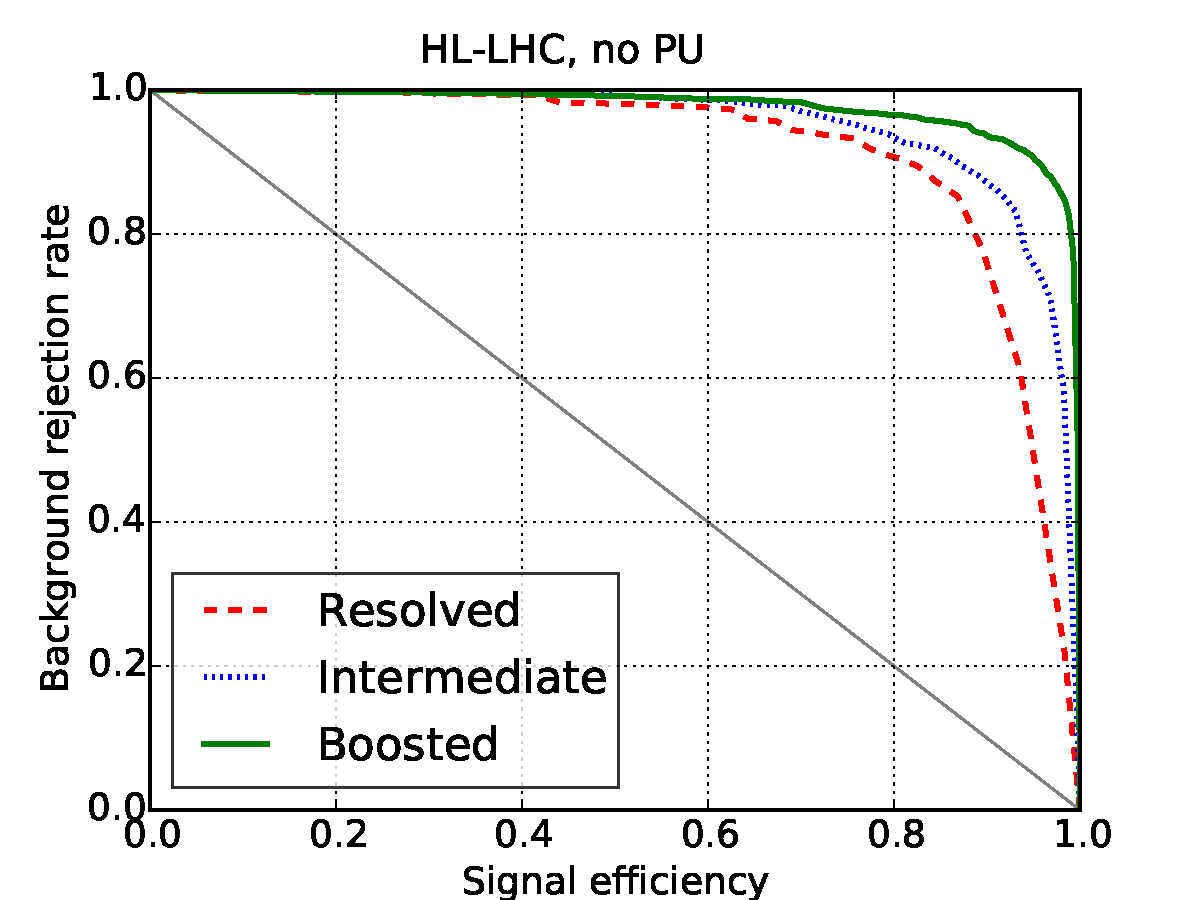
\includegraphics[width=0.49\textwidth]{plots/roc_noPU.pdf}
  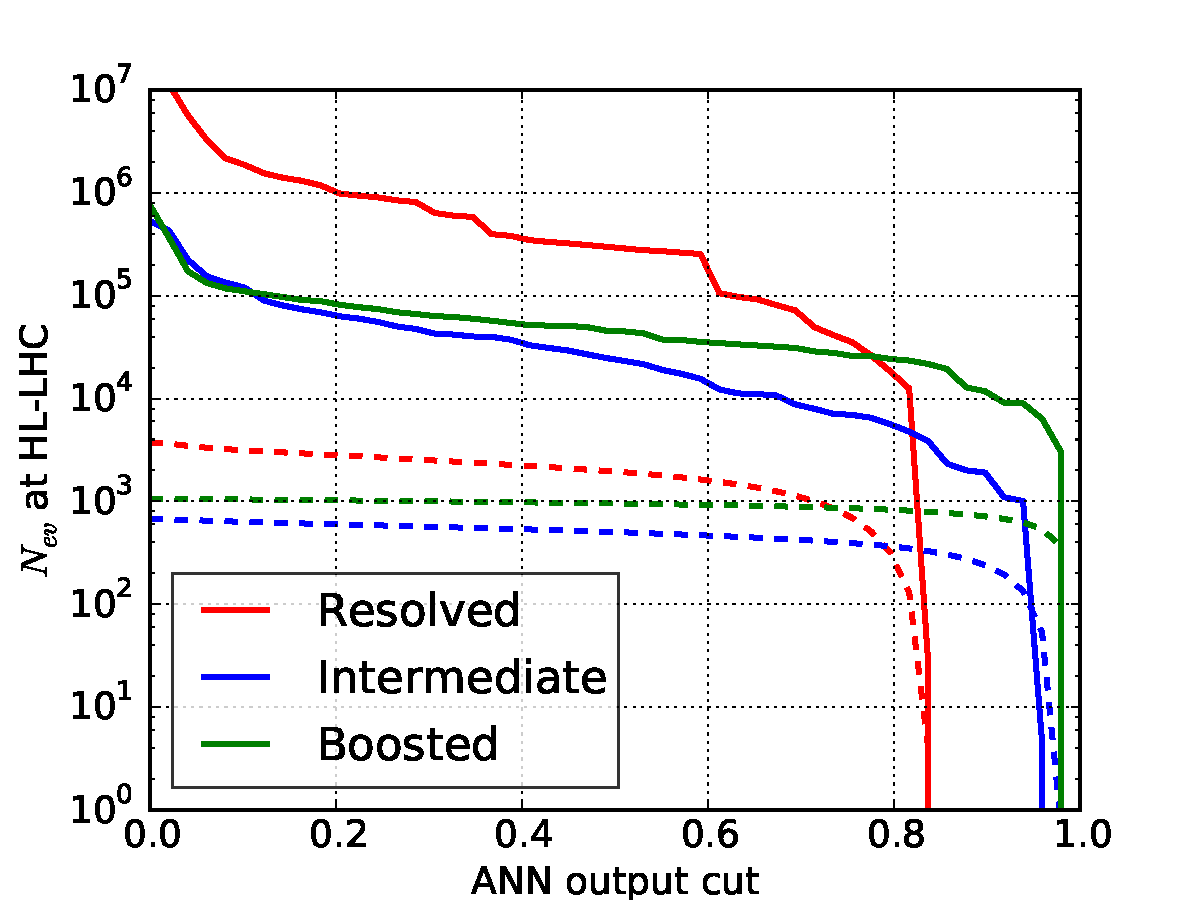
\includegraphics[width=0.49\textwidth]{plots/nev2_noPU.pdf}
\caption{\small Left: ROC curve for the background rejection rate as a function of the signal
  selection efficiency, as the cut $y_{\rm cut}$
  in the ANN output is varied.
  %
  Right: Number of signal (dashed) and background (solid)
  events expected at the HL-LHC as a function of the $y_{\rm cut}$.
}
\label{fig:exampleroc}
\label{fig:nev2}
\end{center}
\end{figure}
%%%%%%%%%%%%%%%%%%%%%%%%%%%%%%%%%%%%%


It important to verify, for each value of
the cut in the ANN output $y_{\rm cut}$, how many
signal and background events are expected at the HL-LHC,
with an integrated luminosity of $\mathcal{L}=3$ ab$^{-1}$.
%
This comparison is shown in 
Fig.~\ref{fig:nev2}.
%
As can be seen,
in the boosted category, for a value $y_{\rm cut}\simeq 0.8$
we end up with 800 signal events and around $2\cdot 10^4$ background
events.
%
Similar results are obtained in the intermediate and resolved
categories: in the former we find 700 ($6\cdot 10^3$) signal (background)
events for $y_{\rm cut}\simeq 0.8$, and in the latter
1300 ($8\cdot 10^4$) signal (background) events for
$y_{\rm cut}\simeq 0.65$.
%
Note that the MVA achieves a very substantial background suppression
with only a
moderate reduction of signal efficiency in exchange.


A useful property of MVAs such as the one used in this work
is that they provide direct  physical insight about which of the
input variables contribute the most to the separation between
signal and background.
%
In the case of ANNs, this can be quantified by computing the sum
of the absolute value of all the weights connected to a given
input neuron $i$, that is
\be
\label{eq:totweight}
\omega^{\rm (tot)}_i \equiv \sum_{k=1}^{n^{(2)}} \Big|\omega^{(2)}_{ki}\Big| \, ,
\qquad i=1,\ldots,N_{\rm var} \, ,
\ee
with $\omega^{(2)}_{ki}$ the value of the weight connecting
the $k$-th neutron of the second layer with the $i$-th neuron of
the first (input) layer, and $n^{(2)}=5$ the number of
neurons in the second layer.
%
Those input variables with a larger value of $\omega^{\rm (tot)}_i$ will be those
that play a dominant role in enhancing the signal
discrimination using the MVA.


%%%%%%%%%%%%%%%%%%%%%%%%
\begin{figure}[t]
  \begin{center}
    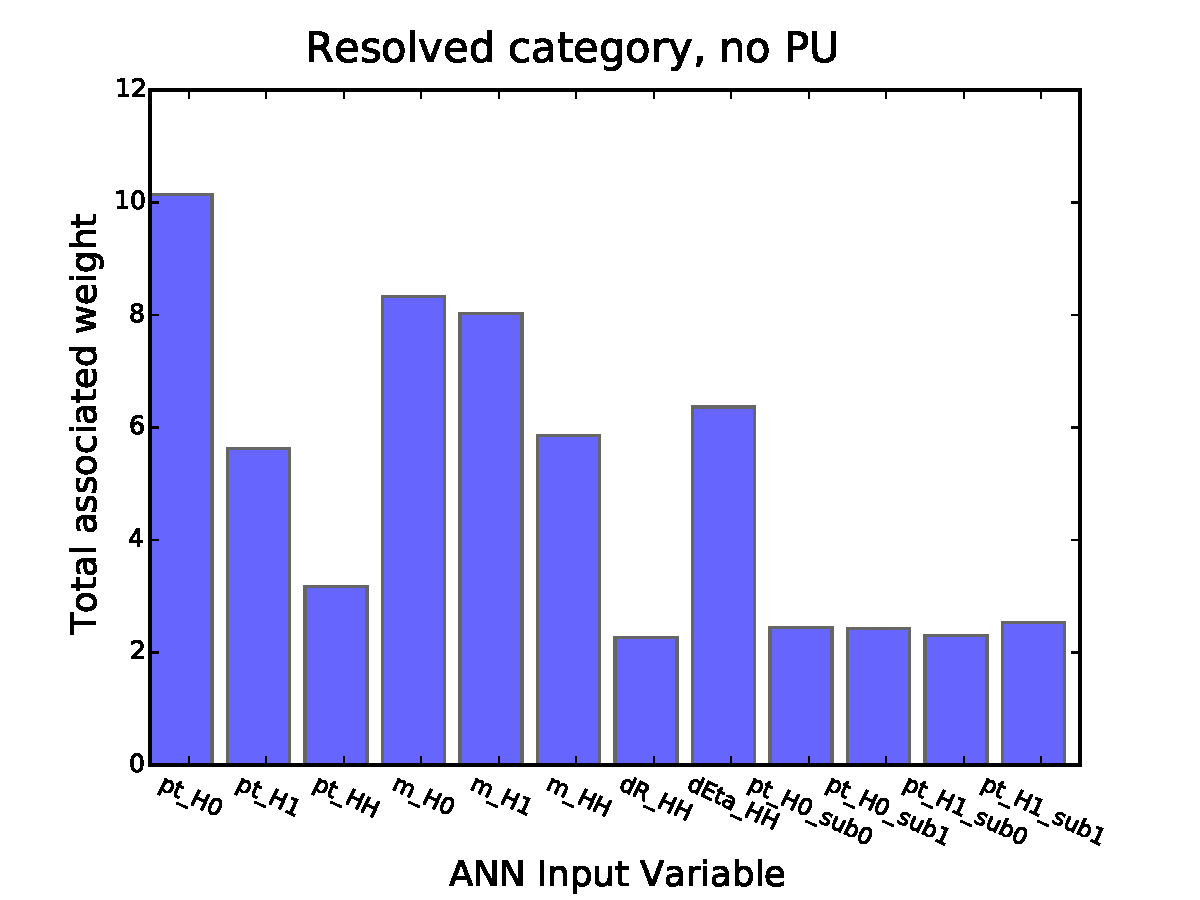
\includegraphics[width=0.49\textwidth]{plots/res_wgthist_noPU.pdf}
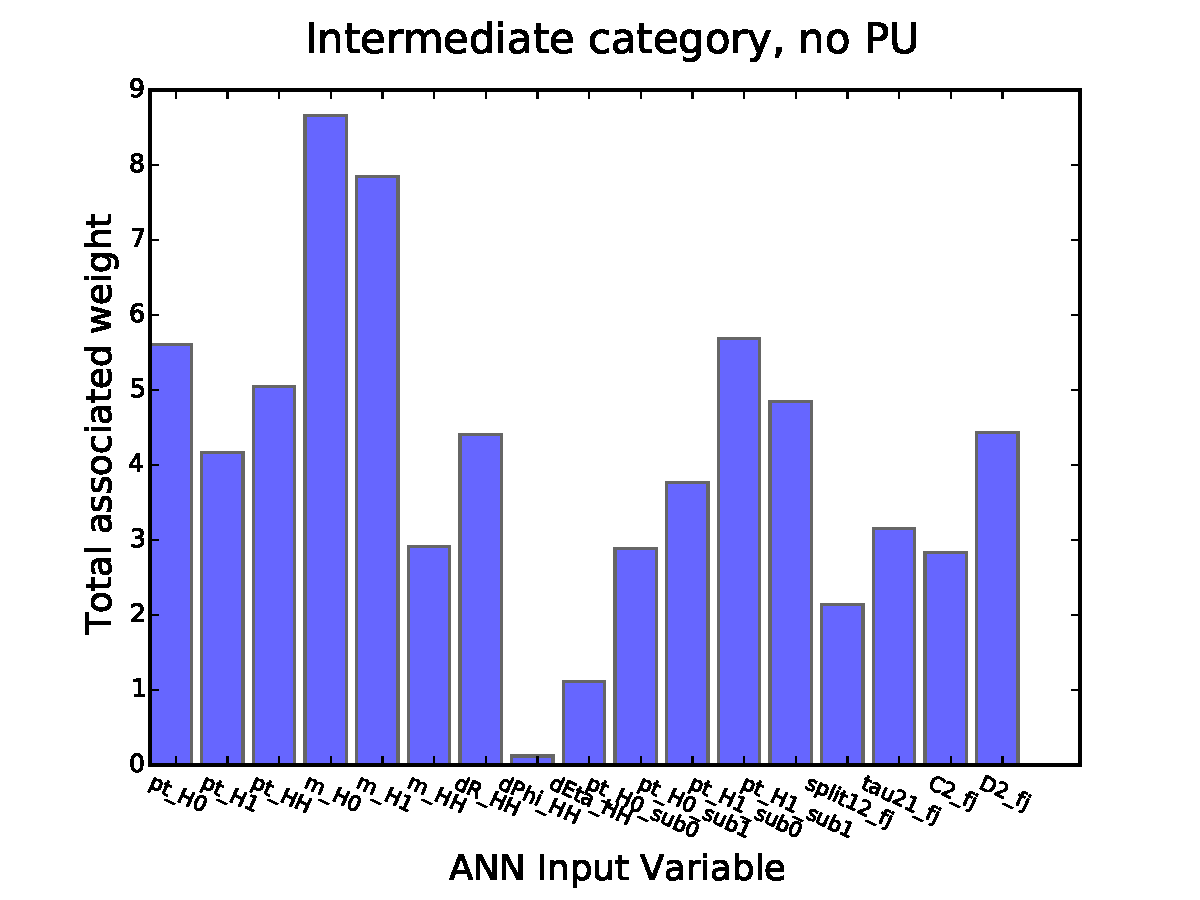
\includegraphics[width=0.49\textwidth]{plots/int_wgthist_noPU.pdf}
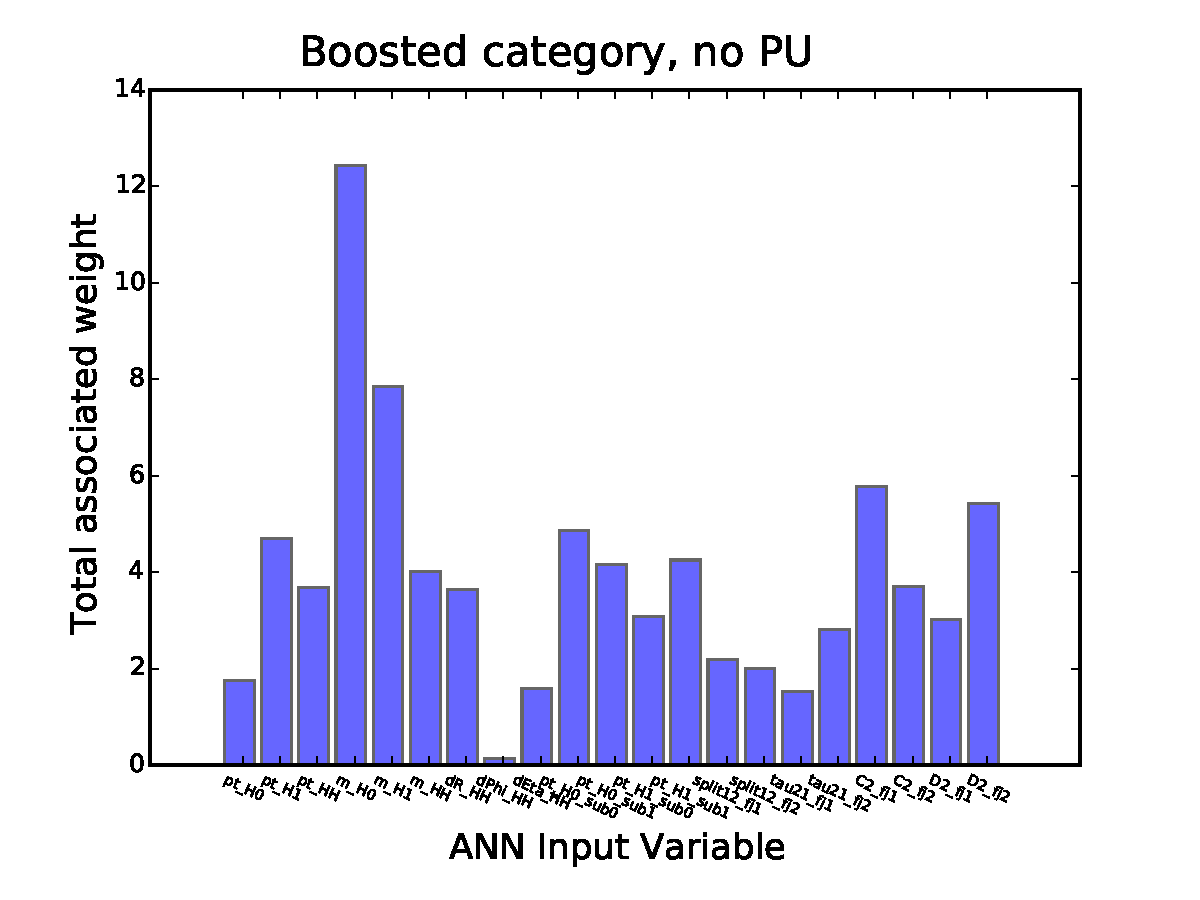
\includegraphics[width=0.75\textwidth]{plots/bst_wgthist_noPU.pdf}
\vspace{-0.5cm}
\caption{\small
Distribution of the total associated weight,
Eq.~(\ref{eq:totweight}) for each of the $N_{\rm var}$ input
variables of the resolved (upper left),  intermediate (upper right)
and boosted (lower plot)
categories.
}
\label{fig:nnweights}
\end{center}
\end{figure}
%%%%%%%%%%%%%%%%%%%%%%%

%
In Fig.~\ref{fig:nnweights} we show
the distribution of the total associated weight,
Eq.~(\ref{eq:totweight}) for each of the $N_{\rm var}$ input
variables of the three categories, using the
notation for the various kinematic variables
as in Sect.~\ref{sec:input}.
%
The important information
is contained in the relative strengths of the total associated weight
for each of the input variables.
%
In the 
resolved category, the variables that carry 
a higher discrimination power
are the $p_T$ of the two reconstructed Higgs candidates and
their invariant masses $m_{h1}$ and $m_{h2}$.
%
In the case of the boosted category, the invariant mass distribution
of the Higgs candidates is also the most discriminatory
variable, followed by the subjet $p_T$ distributions and
substructure variables such as $C_2^{(\beta)}$ and
$D_2^{(\beta)}$.




%%%%%%%%%%%%%%%%%%%%%%%%
\begin{figure}[t]
\begin{center}
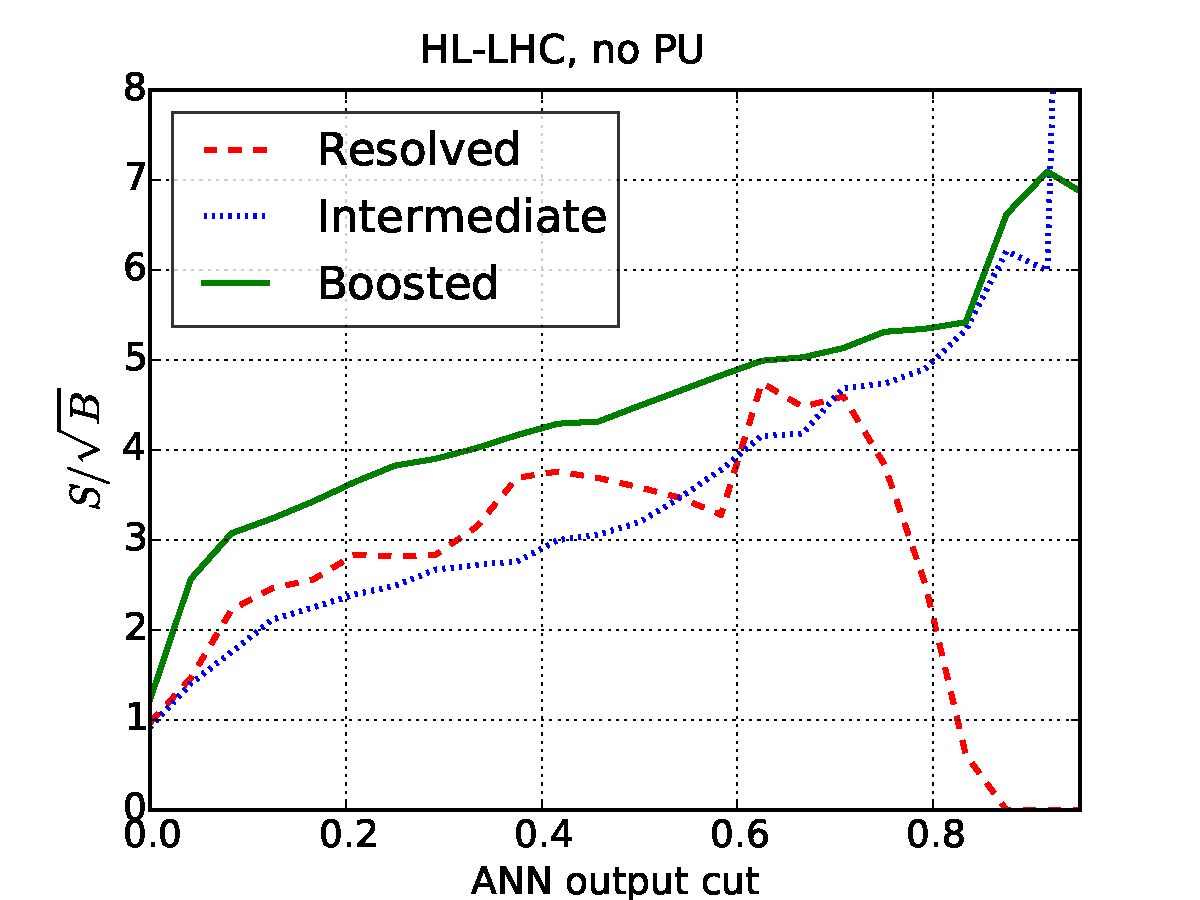
\includegraphics[width=0.48\textwidth]{plots/ssb_noPU.pdf}
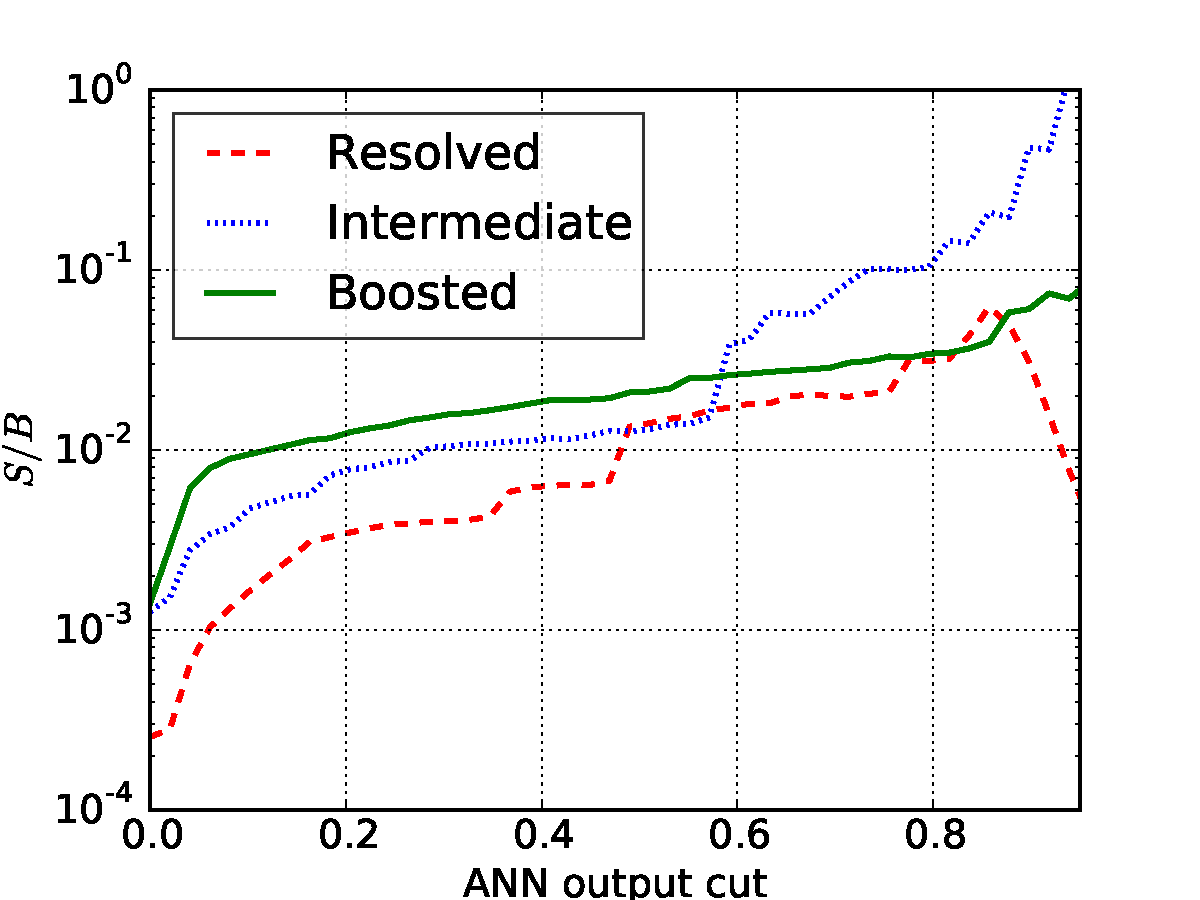
\includegraphics[width=0.48\textwidth]{plots/sb_noPU.pdf}
\caption{\small
  The values of the signal significance, $S/\sqrt{B}$, and of the
  signal over background ratio, $S/B$, for the boosted, intermediate
  and resolved categories as  function of the cut
  $y_{\rm cut}$ in the ANN output.
  %
  The $y_{\rm cut}=0$
  results are those at the end of the cut-based
  analysis.
}
\label{fig:sb_mva}
\end{center}
\end{figure}
%%%%%%%%%%%%%%%%%%%%%%%

The results for the signal significance $S/\sqrt{B}$ and
the signal over background ratio
$S/B$ as a function of $y_{\rm cut}$
for the three categories are
Fig.~\ref{fig:sb_mva}.
%
The values 
for $y_{\rm cut}=0$ correspond to those at
the end of the cut-based analysis.
%
We observe how in the three
 categories there is a marked  improvement in signal
significance as compared to the pre-MVA results.
%
We also observe a substantial enhancement in $S/B$, arising
from the background suppression indeed by the MVA, reaching
values of 1\%, 6\% and 3.5\% in the resolved,
intermediate and boosted categories.
%
This improvement in $S/B$ is crucial to ensure the feasibility
of this measurement, since it allows systematic
uncertainties in the background determination to
be at the same level of a few percent level.

We now have all the
information needed to determine a suitable
value of the MVA output cut $y_{\rm cut}$ in each
of the three categories.
%
These values can be determined from the maximisation of $S/\sqrt{B}$,
ensuring that the number of signal events $N_{\rm ev}$
expected at the HL-LHC is not too small.
%
In  addition, we require
that the number of MC events used to define the signal
category (events with $y_i \ge y_{\rm cut}$)
is large enough to avoid the biases and statistical
fluctuations associated to a small training sample.
%
In Table~\ref{table:cutflowMVA} where we indicate
the value of the optimal ANN output
cut in each category,
the number of signal and background events $N_{\rm ev}$ expected
at the HL-LHC as well as $S/\sqrt{B}$ and $S/B$.
%
For reference, we also include the results at the end of
the cut-based
analysis.
%

%%%%%%%%%%%%%%%%%%%%%%%%%%%%%%%%%%%%%%%%%%%%%%%%%%%%%%%%%%%%%%%%%%%%%%%%%%%%
%%%%%%%%%%%%%%%%%%%%%%%%%%%%%%%%%%%%%%%%%%%%%%%%%%%%%%%%%%%%%%%%%%%%%%%%%%%%
\begin{table}[t]
  \centering
  \begin{tabular}{|c|l|c|c|c|c|}
    \hline
    \multicolumn{6}{|c|}{No PU} \\
    \hline
    \hline
    Category  &   &  $N_{\rm ev}$ signal &  $N_{\rm ev}$ back  &  $S/\sqrt{B}$ & $S/B$ \\ 
    \hline
    \hline
    \multirow{2}{*}{Boosted} &  $y_{\rm cut}=0$  & 1070 & $7.6\cdot 10^5$  & 1.2  & $1.4\cdot 10^{-3}$  \\
    &  $y_{\rm cut}=0.82$ & 790  & $2.2\cdot 10^4$   & 5.4  & 0.034 \\
    \hline
    \hline
    \multirow{2}{*}{Intermediate} &  $y_{\rm cut}=0$  & 670   & $5.3\cdot 10^5$
    & 0.9 & $1.2\cdot 10^{-3}$ \\
    &  $y_{\rm cut}=0.80$ & 360  & $5.5\cdot 10^3$  & 4.8 & 0.06\\
    \hline
    \hline
      \multirow{2}{*}{Resolved} &  $y_{\rm cut}=0$  & 3700 &  $1.5\cdot 10^{7}$ &  1.0 &$3\cdot 10^{-4}$ \\
    &  $y_{\rm cut}=0.65$ & 1300  & $8.3\cdot 10^{4}$ & 4.5 & 0.01 \\
    \hline
      \end{tabular}
  \caption{\small Post-MVA results, for the optimal value of the
    ANN discriminant $y_{\rm cut}$ in the three categories, compared with the
    corresponding
    pre-MVA results $y_{\rm cut}=0$.
    %
    We indicate the number of signal and
    background events
    at the HL-LHC with $\mathcal{L}=3$ ab$^{-1}$,
    the signal significance $S/\sqrt{B}$ and
    the signal over background ratio $S/B$.
    %
    The pre-MVA results ($y_{\rm cut}=0$) corresponds to row C2 in
    Table~\ref{tab:cutflow_noPU_1}.
    \label{table:cutflowMVA}
  }
\end{table}
%%%%%%%%%%%%%%%%%%%%%%%%%%%%%%%%%%%%%%%%%%%%%%%%%%%%%%%%%%%%%%%%%%%%%%%%%%%%
%%%%%%%%%%%%%%%%%%%%%%%%%%%%%%%%%%%%%%%%%%%%%%%%%%%%%%%%%%%%%%%%%%%%%%%%%%%%




From Table~\ref{table:cutflowMVA} we see that at the end of the
MVA the signal significance in the boosted category increases
from 1.2 to 5.4, with $S/B$ increasing from $0.14\%$ to $3.4\%$,
with almost 800 signal events expected at the HL-LHC.
%
For the intermediate and resolved category, $S/\sqrt{B}$
increases from 0.9 and 1.0 to 4.8 and 4.5, with
the signal over background ratio raising from
$0.12\%$ and $0.03\%$ to 6\% and 1\$, respectively.
%
The overall combined significance is thus $S\sqrt{B}\simeq 8$,
well above the threshold for discovery.
%
These remarkable results are however subject to a justified
criticism:
the HL-LHC will be a high-PU environment,
which will affect the description of the various
kinematical distributions used as input to the MVA.
%
Therefore, next we quantify the robustness of the
results summarized Table~\ref{fig:sb_mva}
in a realistic high-PU environment.

\subsection{Impact of PU in the MVA}

In this section we study how the MVA results are modified when
signal and background events are embedded in a high-PU environment.
%
The simulation of PU and the corresponding subtraction with
{\tt SoftKiller} have been performed as described
in Sect.~\ref{sec:pileup}.
%
The cut-based analysis and the subsequent
MVA optimization have been performed using exactly the same
settings as in the case without PU.
%
In Table~\ref{table:cutflowMVA_PU} we provide the results
  at the end of the cut-based analysis,
for the case with $\la n_{\rm PU}\ra=80$+SK.
%
It is clear that the pre-MVA 
signal significance has been degraded
as compared to the case without PU.
%
We now find values for $S/\sqrt{B}$ of 0.25, 0.15 and 0.31, in the resolved,
intermediate and boosted categories, respectively, to be compared
with the corresponding values without PU, namely 1.0, 0.9 and 1.0,
see Table~\ref{table:cutflowMVA}. 
%

Subsequently to 
 the cut-based analysis, the surviving signal and background
MC events in the case of PU are used to re-train the MVA.
%
In Table~\ref{table:cutflowMVA_PU}
we also provide  the number of signal and
    background events expected
    at the HL-LHC with $\mathcal{L}=3$ ab$^{-1}$,
    as well as the
    corresponding values for $S/\sqrt{B}$ and $S/B$,
    for both the cut-based analysis (corresponding
    to $y_{\rm cut}=0$) and after the
    optimal MVA cut, for the simulations
    with $\la n_{\rm PU}\ra=80$
    and SK subtraction.
    %
    From Table~\ref{table:cutflowMVA_PU} we observe that, thanks
to the MVA, the signal significance and the
signal over background ratio are improved from 0.35 and $4\cdot 10^{-4}$
(0.25 and $1\cdot 10^{-4}$) up to 2.9 and 0.034 (2.5 and 0.15)
in the boosted (resolved) category.
%
The intermediate category, on the other hand, exhibits a rather lower post-MVA value of $S/\sqrt{B}$, around
1.1.
%
We thus conclude that, as was already the case
without PU,
the boosted category is the most promising
one for the study of Higgs pair production in the $b\bar{b}b\bar{b}$
final state
at the HL-LHC, also for the case of a high-PU environment, and that
important information will also be obtained from
the resolved category, which has a comparable significance.


%%%%%%%%%%%%%%%%%%%%%%%%%%%%%%%%%%%%%%%%%%%%%%%%%%%%%%%%%%%%%%%%%%%%%%%%%%%%
%%%%%%%%%%%%%%%%%%%%%%%%%%%%%%%%%%%%%%%%%%%%%%%%%%%%%%%%%%%%%%%%%%%%%%%%%%%%
\begin{table}[t]
  \centering
  \begin{tabular}{|c|l|c|c|c|c|}
        \hline
     \multicolumn{6}{|c|}{$\la n_{\rm PU}\ra=80$+SK} \\
     \hline
         \hline
    Category  &   &  $N_{\rm ev}$ signal &  $N_{\rm ev}$ back  &  $S/\sqrt{B}$ & $S/B$ \\ 
    \hline
    \hline
    \multirow{2}{*}{Boosted} &  $y_{\rm cut}=0$  & 360   &  $1.4\cdot 10^6$ & 0.31   &
     $3\cdot 10^{-4}$  \\
    &  $y_{\rm cut}=0.82$ &  250 & 7300  & 2.9    & 0.034  \\
    \hline
    \hline
    \multirow{2}{*}{Intermediate} &  $y_{\rm cut}=0$  &  150  & $9\cdot 10^5$    & 0.15    &
     $2\cdot 10^{-4}$ \\
    &  $y_{\rm cut}=0.80$ & 50 & 2600  &  1.1   & 0.02 \\
    \hline
    \hline
    \multirow{2}{*}{Resolved} &  $y_{\rm cut}=0$  &  1100  & $8.5\cdot 10^6$
    & 0.25    &  $1.3\cdot 10^{-4}$  \\
    &  $y_{\rm cut}=0.65$ & 430  & $3\cdot 10^4$  &  2.5   & 0.015  \\
    \hline
      \end{tabular}
  \caption{\small Same as Table~\ref{table:cutflowMVA}, now for the case
    of PU+SK, with $\la n_{\rm PU}\ra=80$.
        \label{table:cutflowMVA_PU}
  }
\end{table}
%%%%%%%%%%%%%%%%%%%%%%%%%%%%%%%%%%%%%%%%%%%%%%%%%%%%%%%%%%%%%%%%%%%%%%%%%%%%
%%%%%%%%%%%%%%%%%%%%%%%%%%%%%%%%%%%%%%%%%%%%%%%%%%%%%%%%%%%%%%%%%%%%%%%%%%%%

Another important result from Table~\ref{table:cutflowMVA_PU} is that,
for the optimal MVA cut, the signal over background ratio
is not unfeasibly small: we obtain that $S/B$ is 3.4\% (1.5\%)
in the boosted (resolved) categories.
%
This is indicates that while this measurement is still very challenging,
requiring a careful extraction from the data of the QCD
background, it is certainty within reach.
%
As in the case without PU, 
this analysis  indicates that a substantial increase in both
$S/B$ and $S/\sqrt{B}$ could be achieved by reducing the background component
that arises from the mis-identification of light and charm
fakes.

In Fig.~\ref{fig:nev2_PU}
we show the number of signal and background events that
are expected at the HL-LHC as a function of
$y_{\rm cut}$ and the corresponding ROC curve
%
Comparing Figs.~\ref{fig:nev2} and~\ref{fig:nev2_PU}, we observe
that the intermediate category is substantially degraded once PU effects
are accounted for, the reason being  sizable
a reduction in the number of signal
events that are now assigned to this category.
%
This shows that the selection criteria
of the intermediate category are less
resilient against PU contamination,
as opposed to the resolved and boosted selections.

%%%%%%%%%%%%%%%%%%%%%%%%%%%%%%%%%%%%%%%%%%%%%
\begin{figure}[t]
  \begin{center}
    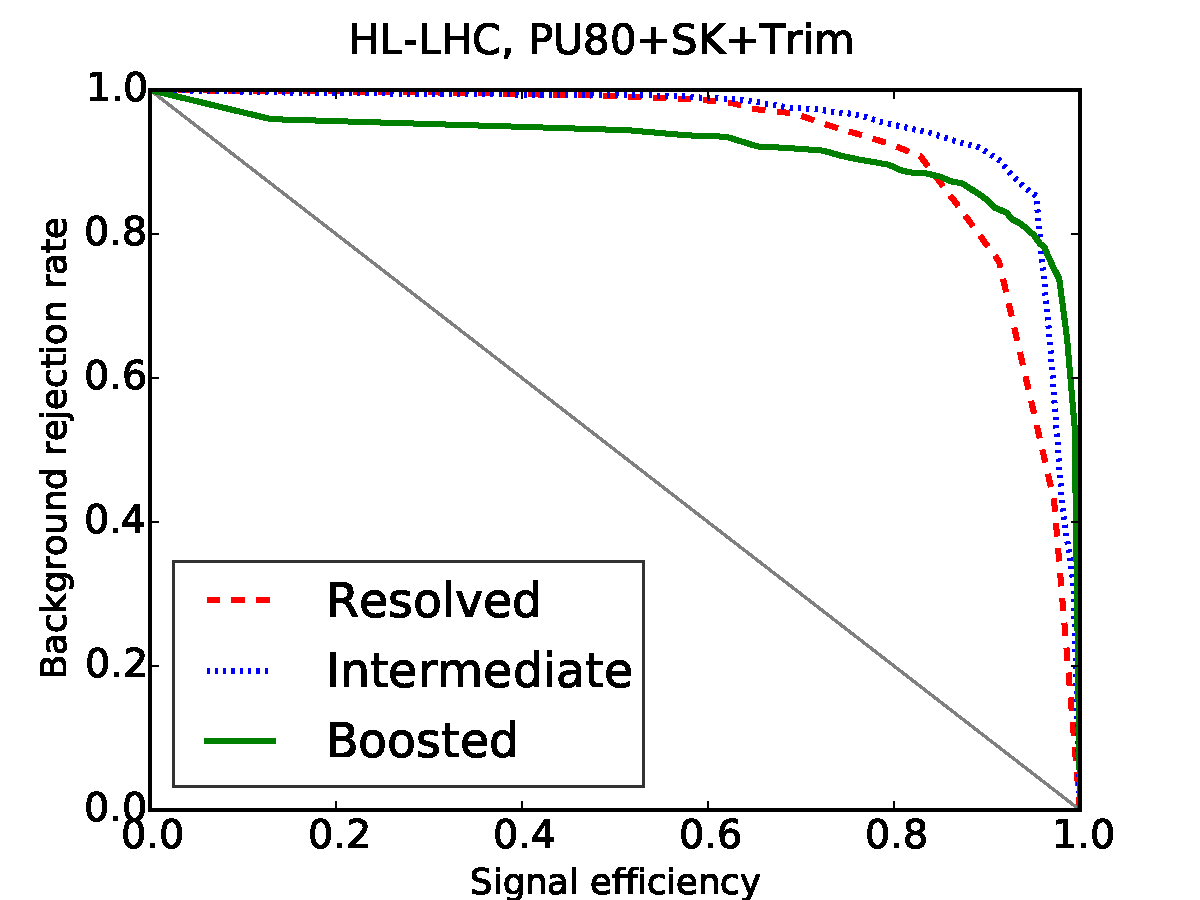
\includegraphics[width=0.49\textwidth]{plots/roc_SKPU80.pdf}
\includegraphics[width=0.49\textwidth]{plots/nev2_SKPU80.pdf}
\caption{\small Same as Fig.~\ref{fig:nev2} in the
case of events with PU, for
 $\la n_{\rm PU}\ra=80$ 
  and SK subtraction.
}
\label{fig:nev2_PU}
\end{center}
\end{figure}
%%%%%%%%%%%%%%%%%%%%%%%%%%%%%%%%%%%%%


In Fig.~\ref{fig:sb_mva_PU} we show the signal significance,
$S/\sqrt{B}$, as well as the signal over background ratio,
$S/B$, including now the effects of PU.
%
The corresponding results in the case without PU were shown in
Fig.~\ref{fig:sb_mva}.
%
As can be seen, the MVA-driven enhancement is robust in the
presence of PU.
%
While unsurprisingly there us a degradation as compared to the case wo PU,
we still manage to achieve a signal significance of
around $S/\sqrt{B}$ between 2.5 and 3.0
separately for the boosted and resolved
categories.
%
On the other hand, the intermediate category becomes marginal.
%
We conclude that the qualitative conclusions drawn in
Sect.~\ref{sec:mva} are robust in the presence
of realistic PU effects.
%
Since no specific effort has been performed to
optimize PU subtraction, for example by tuning the value
of the patch length $a$ in {\tt SoftKiller}, we believe that
there is
still room for improvement in this respect.


%%%%%%%%%%%%%%%%%%%%%%%%%%%%%%%%%%%%%%%%%%%%%%%%%%%%
%%%%%%%%%%%%%%%%%%%%%%%%%%%%%%%%%%%%%%%%%%%%%%%%%%%%
\begin{figure}[t]
\begin{center}
\includegraphics[width=0.48\textwidth]{plots/ssb_SKPU80.pdf}
\includegraphics[width=0.48\textwidth]{plots/sb_SKPU80.pdf}
\caption{\small 
Same as Fig.~\ref{fig:sb_mva} in the
case of events with PU, for
 $\la n_{\rm PU}\ra=80$ 
  and SK subtraction.
}
\label{fig:sb_mva_PU}
\end{center}
\end{figure}
%%%%%%%%%%%%%%%%%%%%%%%

It is important to quantify which of the input variables
to the MVA carry the highest discrimination power
in the case of PU,
and compare it with the corresponding
results without PU.
%
We use the same estimator as in Sect.~\ref{sec:signalsignificance},
namely the sum
of the absolute value of all the weights connected to a given
input neuron $i$, Eq.~(\ref{eq:totweight}).
%
The results for the resolved and boosted categories are shown
on Fig.~\ref{fig:nnweights_PU}.
%
As we can see by comparing to the corresponding
results without PU in Fig.~\ref{fig:nnweights}, 
in the boosted category, the discrimination power of the invariant
mass of Higgs candidates is decreased and that of the various substructure
variables, in particular $C_2^{(\beta)}$ and
$D^{(\beta)}$, is conversely
increased.
%
This reflects the fact that these substructure variables are
relatively robust against PU contamination.
%
In addition, also the $p_T$ distributions of the AKT03
subjets within the large-$R$
jets carry important information.
%
In the case of the resolved category,  the highest
values of the ANN weights without PU
were found for the $p_T$ of the leading
Higgs and for the Higgs invariant masses.
%
This is also true in the case with PU, but now the rapidity difference
between the two Higgs candidates, $\Delta y_{hh}$ increases its
importance, again reflecting that this variable is relatively
insensitive to PU effects.
%

%%%%%%%%%%%%%%%%%%%%%%%%
\begin{figure}[t]
\begin{center}
\includegraphics[width=0.49\textwidth]{plots/res_wgthist_SKPU80.pdf}
\includegraphics[width=0.49\textwidth]{plots/bst_wgthist_SKPU80.pdf}
\vspace{-0.5cm}
\caption{\small
Same as Fig.~\ref{fig:nnweights} in the
case of events with PU, for
 $\la n_{\rm PU}\ra=80$ 
  and SK subtraction.
}
\label{fig:nnweights_PU}
\end{center}
\end{figure}
%%%%%%%%%%%%%%%%%%%%%%%

We can finally combine the three categories, resolved,
intermediate and boosted, and determine the overall signal
significance, finding
\be
\lp \frac{S}{\sqrt{B}}\rp_{\rm tot} \simeq 4.0 \, ,
\ee
to be compared to the value $\lp S/\sqrt{B}\rp_{\rm tot} \simeq 8.5$
that was obtained in the case without PU.
%
We conclude that, even when realistic PU effects are accounted
for, at the HL-LHC the measurement of
Higgs pair production in the $b\bar{b}b\bar{b}$ final state should be 
well the threshold for evidence, and even meeting the
requirements for discovery might be within reach provided it is possible
to suppress the background from light and charm jet mis-identifications.


For the Run II luminosity, $\mathcal{L}=300$ fb$^{-1}$, one finds
instead $\lp S/\sqrt{B}\rp_{\rm tot} \simeq 1.3$, which increases up to
$\lp S/\sqrt{B}\rp_{\rm tot} \simeq 2.6$ if only the QCD $4b$ background is included.
%
This indicates that, interestingly, accessing Higgs pair production at Run II,
while still extremely challenging, does not seem to be completely impossible.
%
In addition, at Run II the average number of PU collisions is substantially
reduced as compared to the HL-LHC environment.
%
Therefore, it will be interesting to see if improvements in experimental $b$-jet
reconstruction and fake rejection at Run II are able to fulfill this
potential.

%%%%%%%%%%%%%%%%%%%%%%%%%%%%%%%%%%%%%%%%%%%%%%%%%%%%%%%%%%%%%%%%%%%%%%%%%%%%%%%%
%%%%%%%%%%%%%%%%%%%%%%%%%%%%%%%%%%%%%%%%%%%%%%%%%%%%%%%%%%%%%%%%%%%%%%%%%%%%%%%%
%%%%%%%%%%%%%%%%%%%%%%%%%%%%%%%%%%%%%%%%%%%%%%%%%%%%%%%%%%%%%%%%%%%%%%%%%%%%%%%%
%%%%%%%%%%%%%%%%%%%%%%%%%%%%%%%%%%%%%%%%%%%%%%%%%%%%%%%%%%%%%%%%%%%%%%%%%%%%%%%%
%%%%%%%%%%%%%%%%%%%%%%%%%%%%%%%%%%%%%%%%%%%%%%%%%%%%%%%%%%%%%%%%%%%%%%%%%%%%%%%%


\section{Optimisation}
\label{sec:optimisation}

One important motivation of this work was to quantify which aspects
of the performance of the LHC detectors needs to be improved
the most in order to maximise the significance of the observation
of double Higgs production in the $4b$ final state.
%
In this section we explore how the results with the baseline settings,
summarized in the previous section, are modified when some of
these settings are changed.
%
In particular we will explore the dependence of the results on
the $b$-tagging probability $f_b$, the light jet mistag rate
$f_l$, as well on the momentum smearing fraction.
%
The variations of the analysis
settings that we will explore are collected in
Table~\ref{sec:variations}.

%%%%%%%%%%%%%%%%%%%
\begin{table}[h]
  \centering
  \begin{tabular}{|c|c|c|c|}
\hline
    Scenario  &  $f_b$  &  $f_l$  &  $\Delta p_T$ \\
    \hline
    \hline
    Baseline  &  0.8   &   0.01  &  5\% \\
    \hline
    A        &  0.9   &   0.01  &  5\% \\
    B        &  0.7   &   0.01  &  5\% \\
    C        &  0.8   &   0.005  &  5\% \\
    D        &  0.8   &   0.02  &  5\% \\
    E        &  0.9   &   0.005  &  2\% \\   
    \hline
  \end{tabular}
  \caption{\small The baseline settings for the $b$-jet
    tagging probability, the light jet mistag rate $f_l$
    and the $p_T$ resolution $\Delta p_T$, compared
    to the various scenarios that we discusse in this section.
\label{sec:variations}
  }
  \end{table}
%%%%%%%%%%%%%%%%%%%

\section{Conclusions and outlook}
\label{sec:conclusions}

In this work we have presented a feasibility study for
 the measurement of Higgs pair production in the $b\bar{b}b\bar{b}$
final state at the High-Luminosity LHC with $\mathcal{L}=3$ ab$^{-1}$.
%
Our strategy is based on the combination of traditional
cut-based analysis with state-of-the-art multivariate techniques.
%
We take into account 
all relevant backgrounds, in particular
the irreducible $4b$
and the reducible 
$2b2j$ and $4j$ QCD multijets.
%
We have illustrated how the $2b2j$ component leads to
a contribution comparable to that of the $4b$ process,
due to a combination of  parton shower effects, $b$-quark 
pair radiation, and selection requirements.
%
We have also demonstrated the robustness of our analysis strategy
under the addition of significant pileup.

Combining the contributions from the resolved,
intermediate and boosted categories, we find that, for
$\mathcal{L}=3$ ab$^{-1}$, the
signal significance for
the production of Higgs pairs can be as large as $S/\sqrt{B}\simeq 4.0$.
%
This indicates that, already from the $b\bar{b}b\bar{b}$
final state alone,
it should be possible to claim evidence for Higgs pair production at
the HL-LHC.
%
Our study also suggests possible avenues that the LHC experiments
could explore to further improve this signal significance.
%
One handle would be to reduce the contribution from light and charm
jet mis-identification, ensuring that the irreducible $4b$ background 
 dominates over the $2b2j$ component.
%
Another possibility would be to improve the mass resolution of the Higgs
reconstruction
in high-PU environments, and, more in general,
to optimize the PU subtraction
strategy in order
to reduce the impact of PU in the modelling
of kinematical variables and the associated
degradation in the MVA discrimination.
%
Such experimental improvements might
even make
an observation of Higgs pair production possible at the
end of Run II with
$\mathcal{L}=300$ fb$^{-1}$.

One important implication of this work is that it should
be possible to improve  the accuracy on the extraction of
the Higgs trilinear coupling $\lambda$ from
a measurement of the
$\sigma\lp hh\to b\bar{b}b\bar{b}\rp$ cross-section, as compared
to existing estimates.
%
A determination of $\lambda$ in our approach is however
rather
non-trivial, involving
 not only regenerating signal samples
 for a wide range of values of  $\lambda$, but also
 repeating the analysis
optimisation, including the MVA training, for each
of these values.
%
This study is left to a future
publication, where we will also
compare with the corresponding  precision 
that has been reported from other final states such as
 $b\bar{b}\gamma\gamma$
and $b\bar{b}\tau\tau$.
%
It will also be  interesting to perform
this exercise for a 100 TeV hadron collider~\cite{Barr:2014sga,
  Azatov:2015oxa,Papaefstathiou:2015iba,
  Arkani-Hamed:2015vfh}.
%
While signal yields will be certainly increased, also the (gluon-driven) QCD
multijet background will grow strongly.
%
Revisiting
the present analysis, including the MVA optimization,
at 100 TeV will allow us
to assess the accuracy of an extraction of the trilinear
coupling $\lambda$ from the $b\bar{b}b\bar{b}$ final state
at 100 TeV.


Our strategy relies on the modeling of the kinematical
distributions of signal and background events, since these provide
the inputs to the MVA discriminant.
%
In this respect, it would be important, having established the key
relevance of the $b\bar{b}b\bar{b}$ channel for the study of
Higgs pair production, to revisit and improve the
theoretical modeling of our signal and background simulation,
in particular using NLO calculations matched to
parton showers both for signal~\cite{Frederix:2014hta,Maierhofer:2013sha}
and for backgrounds~\cite{Alwall:2014hca,Gleisberg:2008ta}.
%

In this work we have considered only the SM production mechanism,
but many BSM scenarios predict deviations
in Higgs pair production, both at the level of total rates
and of
differential distributions.
%
In the absence of new explicit degrees of freedom,
deviations from the SM can be parametrized in
the EFT framework using higher-order
operators~\cite{Azatov:2015oxa,Goertz:2014qta}.
%
Therefore, we plan to study the constraints
on the coefficients of these effective
operators that can be obtained from measurements
of various kinematical distributions
in the $hh\to b\bar{b}b\bar{b}$ process.
%
Note that the higher rates of the $b\bar{b}b\bar{b}$ final state as compared to
other final states, such as
$b\bar{b}\gamma\gamma$, allow for a better constraint upon operators
that modify the high-energy behavior
of the theory, for instance,
it would become possible
to access the tail of the $m_{hh}$ distribution.


As in the case of the extraction of the Higgs
trilinear coupling $\lambda$, such a study
would be a computationally intensive task, since
BSM dynamics will modify the shapes of the kinematical
distributions and thus in principle each point in the EFT parameter
space would require a re-optimization with a newly trained
MVA.
%
In order to explore efficiently the BSM parameters
without having to repeat the full analysis
for each point, modern statistical techniques
such as the Cluster Analysis method proposed
in Ref.~\cite{Dall'Osso:2015aia} might be helpful.



\bigskip
\bigskip
\begin{center}
\rule{5cm}{.1pt}
\end{center}
\bigskip
\bigskip

{\bf\noindent  Acknowledgments \\}
We thank F.~Bishara, R.~Contino, A.~Papaefstathiou and
G.~Salam for useful discussions on the topic
of Higgs pair production.
%
We thank E.~Vryonidou and M.~Zaro for
assistance with di-Higgs production
  in {\tt MadGraph5\_aMC@NLO}.
%
  J.~R. is supported by an STFC Rutherford Fellowship and
  Grant ST/K005227/1 and ST/M003787/1.
%
J.~R. and N.~H. are
supported by an European Research Council Starting Grant ``PDF4BSM".
%
K.~B. is supported by a Rhodes Scholarship.
%
D.~B., J.~F. and C.~I. are supported by the STFC.


\appendix
\section{sec-appendix-overlap}

\bibliography{HH4b}



\end{document}
